\documentclass[11pt]{elegantbook}
\definecolor{structurecolor}{RGB}{40,58,129}
\linespread{1.6}
\setlength{\footskip}{20pt}
\setlength{\parindent}{0pt}
\newcommand{\argmax}{\operatornamewithlimits{argmax}}
\newcommand{\argmin}{\operatornamewithlimits{argmin}}
\elegantnewtheorem{proof}{Proof}{}{Proof}
\elegantnewtheorem{claim}{Claim}{prostyle}{Claim}
\DeclareMathOperator{\col}{col}
\title{\textbf{Microeconomic Theory}}
\author{Wenxiao Yang}
\institute{Haas School of Business, University of California Berkeley}
\date{2023}
\setcounter{tocdepth}{2}
\cover{cover.png}
\extrainfo{All models are wrong, but some are useful.}

% modify the color in the middle of titlepage
\definecolor{customcolor}{RGB}{9,119,119}
\colorlet{coverlinecolor}{customcolor}
\usepackage{cprotect}

\addbibresource[location=local]{reference.bib} % bib

\begin{document}

\maketitle
\frontmatter
\tableofcontents
\mainmatter




\chapter{Correspondence: $\Psi : X \rightarrow 2^Y$ \small{(@ Lec 07 of ECON 204)}}
\begin{definition}[Correspondence]
    \normalfont
    A \textbf{correspondence} $\Psi : X \rightarrow 2^Y$ from $X$ to $Y$ is a function from $X$ to $2^Y$, that is, $\Psi(x) \subseteq Y$ for every $x \in X$. ($2^Y$ is the set of all subsets of $Y$)
\end{definition}
\begin{example}
Let $u : \mathbb{R}_+^n \rightarrow \mathbb{R}$ be a continuous utility function, $y > 0$ and $p \in \mathbb{R}_{++}^n$, that is, $p_i > 0$ for each $i$. Define $\Psi : \mathbb{R}_{++}^n \times \mathbb{R}_{++} \rightarrow 2^{\mathbb{R}_{+}^n}$ by
\begin{equation}
    \begin{aligned}
        \Psi(p,y)=&\argmax u(x)\\
        \textnormal{s.t. }&x\geq 0\\
        &p\cdot x\leq y
    \end{aligned}
    \nonumber
\end{equation}
$\Psi$ is the demand correspondence associated with the utility function $u$; typically $\Psi(p, y)$ is multi-valued.
\end{example}

\section{Continuity of Correspondences}
\subsection{Upper/Lower Hemicontinuous}
Let $X\subseteq \mathbb{E}^n$, $Y\subseteq \mathbb{E}^m$, and $\Psi: X \rightarrow 2^Y$.
\begin{definition}[Upper Hemicontinuous]
    \normalfont
    $\Psi$ is \textbf{upper hemicontinuous} (uhc) at $x_0 \in X$ if, for every \underline{open set} $V$ with $\Psi(x_0)\subseteq V$, there is an \underline{open set} $U$ with $x_0 \in U$ s.t.
    $$x\in U \Rightarrow \Psi(x)\subseteq V$$
\end{definition}
Upper hemicontinuity reflects the requirement that $\Psi$ doesn't “jump down/implode in the limit” at $x_0$. \textit{(A set to “jump down” at the limit $x_0$: It should mean the set suddenly gets smaller -- it “implodes in the limit” -- that is, there is a sequence $x_n \rightarrow x_0$ and points $y_n \in \Psi(x_n)$ that are far from every point of $\Psi(x_0)$ as $n \rightarrow \infty$.)}
\begin{definition}[Lower Hemicontinuous]
    \normalfont
    $\Psi$ is \textbf{lower hemicontinuous} (lhc) at $x_0 \in X$ if, for every \underline{open set} $V$ with $\Psi(x_0)\cap V \neq \emptyset$, there is an \underline{open set} $U$ with $x_0 \in U$ s.t.
    $$x\in U \Rightarrow \Psi(x)\cap V\neq \emptyset$$
\end{definition}
Lower hemicontinuity reflects the requirement that $\Psi$ doesn't “jump up/explode in the limit” at $x_0$. \textit{(A set to “jump up” at the limit $x_0$: It should mean that the set suddenly gets bigger -- it “explodes in the limit” -- that is, there is a sequence $x_n \rightarrow x_0$ and a point $y_0\in\Psi(x_0)$ that is far from every point of $\Psi(x_n)$ as $n \rightarrow \infty$.)}

\begin{definition}[Continuous Correspondence]
    \normalfont
    $\Psi$ is \textbf{continuous} at $x_0 \in X$ if it is both \textbf{uhc} and \textbf{lhc} at $x_0$.
\end{definition}

\begin{proposition}
    $\Psi$ is upper hemicontinuous (respectively lower hemicontinuous, continuous) if it is uhc (respectively lhc, continuous) at every $x \in X$.
\end{proposition}

\begin{center}\begin{figure}[htbp]
    \centering
    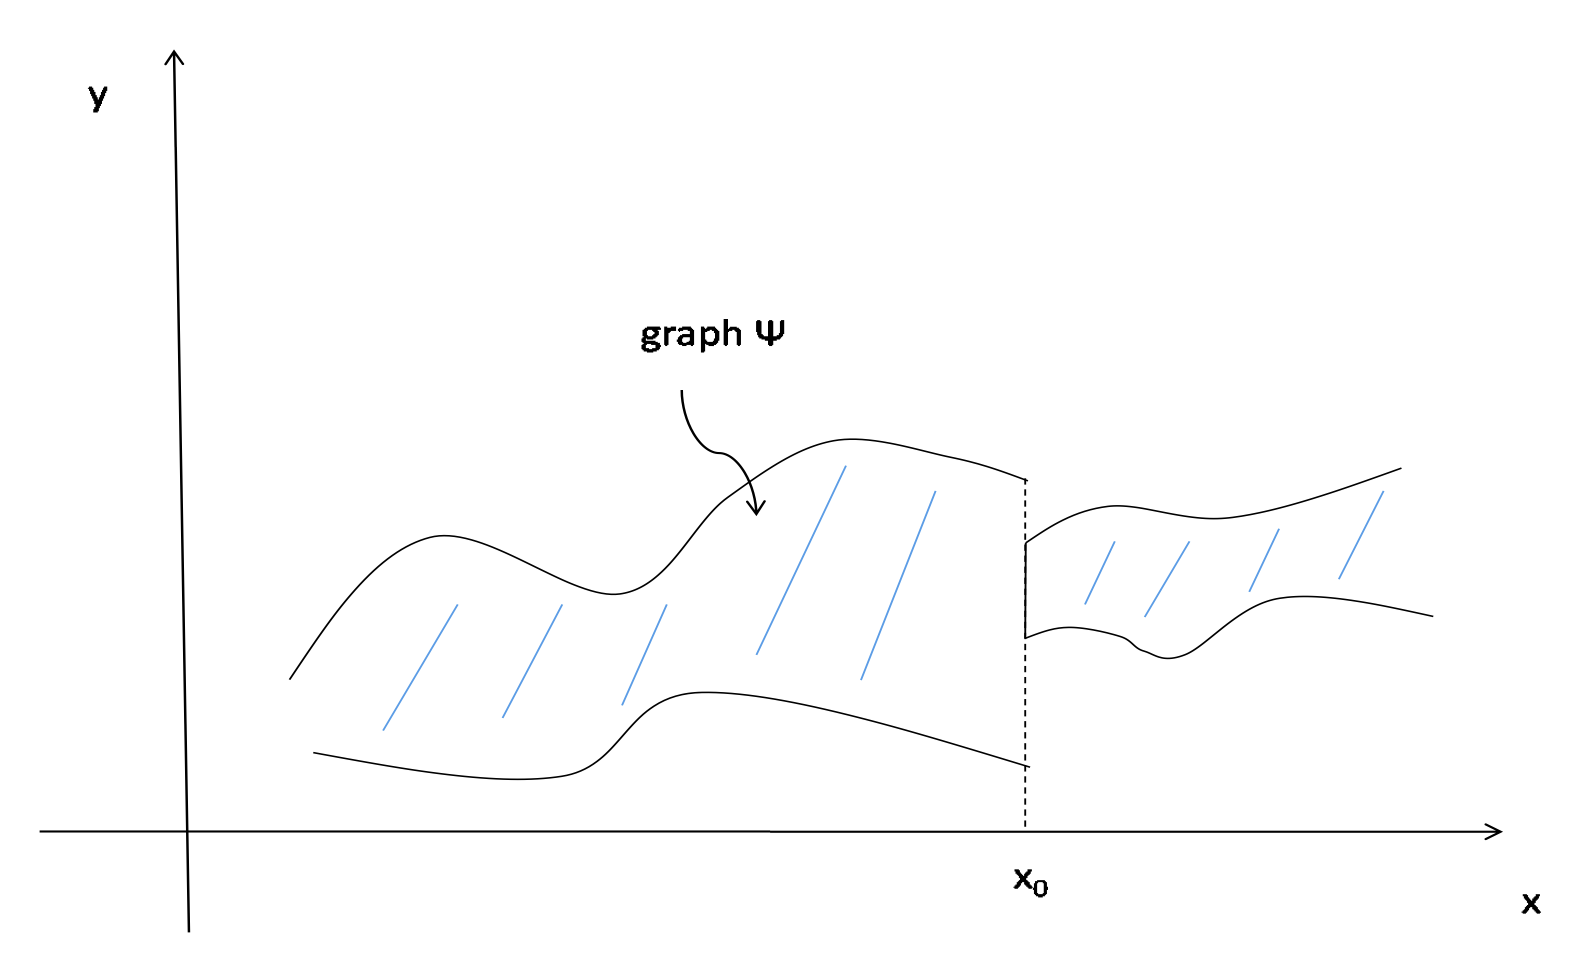
\includegraphics[scale=0.2]{uhc.png}
    \caption{The correspondence $\Psi$ “implodes in the limit” at $x_0$. $\Psi$ is not upper hemicontinuous at $x_0$.}
    \label{}
\end{figure}\end{center}

\begin{center}\begin{figure}[htbp]
    \centering
    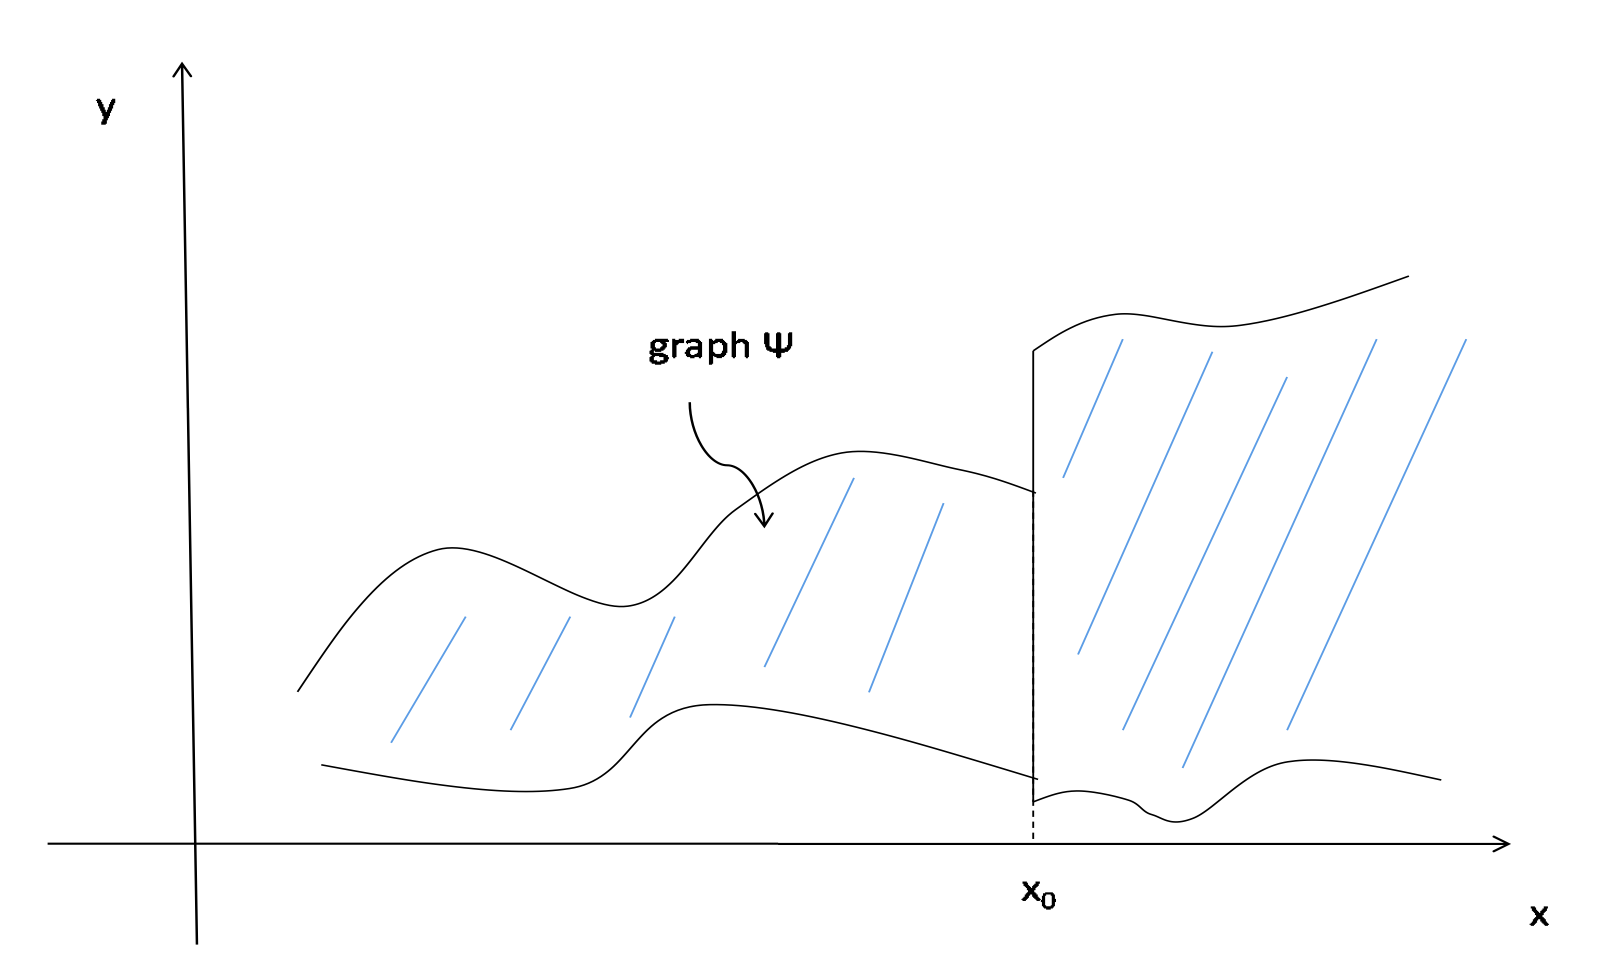
\includegraphics[scale=0.2]{lhc.png}
    \caption{The correspondence $\Psi$ “explodes in the limit” at $x_0$. $\Psi$ is not lower hemicontinuous at $x_0$.}
    \label{}
\end{figure}\end{center}

\subsection{Theorem: $\Psi(x)=\{f(x)\}$ is uhc $\Leftrightarrow$ $f$ is continuous}
\begin{theorem}[$\Psi(x)=\{f(x)\}$ is uhc $\Leftrightarrow$ $f$ is continuous]
    Let $X \subseteq \mathbb{E}^n$, $Y \subseteq \mathbb{E}^m$ and $f : X \rightarrow Y$. Let $\Psi : X \rightarrow  2^Y$ be defined by $\Psi(x) = \{f(x)\}$ for all $x \in X$. Then $\Psi$ is \textbf{uhc} \underline{if and only if} $f$ is \textbf{continuous}.
\end{theorem}


\subsection{Berge's Maximum Theorem: the set of maximizers is uhc with non-empty compact values}
\begin{theorem}[Berge's Maximum Theorem]\label{thm:Berge's Maximum Theorem}
    Let $X \subseteq \mathbb{R}^n$ and $Y \subseteq \mathbb{R}^m$. Consider the function $f : X \times Y \rightarrow \mathbb{R}$ and the correspondence $\Gamma : Y \rightarrow 2^X$. Define $v(y) = \max_{x\in\Gamma(y)} f(x, y)$ and the set of maximizers $$\Omega(y) = \argmax_{x\in\Gamma(y)} f(x, y)=\{x:f(x,y)=v(y)\}$$
    Suppose $f$ and $\Gamma$ are continuous, and that $\Gamma$ has non-empty compact values. Then, $v$ is continuous and $\Omega$ is uhc with non-empty compact values.
\end{theorem}




\section{Graph of Correspondence}
An alternative notion of continuity looks instead at properties of the graph of the correspondence.
\begin{definition}[Graph of Correspondence]
    \normalfont
    The \textbf{graph} of a correspondence $\Psi : X \rightarrow 2^Y$ is the set
    $$\textnormal{graph}\Psi=\{(x,y)\in X\times Y:y\in\Psi(x)\}$$
\end{definition}

\subsection{Closed Graph}
By the definition of continuous function $f:\mathbb{R}^n \rightarrow \mathbb{R}$,  each convergent sequence $\{(x_n, y_n)\}$ in graph $f$ converges to a point $(x, y)$ in graph $f$, that is, graph $f$ is closed.

\begin{definition}[Closed Graph]
    \normalfont
    Let $X\subseteq \mathbb{E}^n$, $Y\subseteq \mathbb{E}^m$. A correspondence $\Psi: X \rightarrow 2^Y$ has closed graph if its graph is a closed subset of $X \times Y$, that is, if for any sequences $\{x_n\} \subseteq X$ and $\{y_n\} \subseteq Y$ such that $x_n \rightarrow x \in X$, $y_n \rightarrow y \in Y$ and $y_n \in \Psi(x_n)$ for each $n$, then $y \in \Psi(x)$.
\end{definition}
\begin{example}
    Consider the correspondence $\Psi(x)=\left\{\begin{matrix}
        \{\frac{1}{x}\},&\textnormal{ if }x\in(0,1]\\
        \{0\},&\textnormal{ if }x=0
    \end{matrix}\right.$ ("implode in the limit")\\
    Let $V = (-0.1, 0.1)$. Then $\Psi(0) = \{0\} \subseteq V$, but no matter how close $x$ is to $0$, $\Psi(x)=\{\frac{1}{x}\}\nsubseteq V$, so $\Psi$ is not uhc at $0$. However, note that $\Psi$ has closed graph.
\end{example}

\section{Closed-valued, Compact-valued, and Convex-valued Correspondences}
\begin{definition}[Closed-valued, Compact-valued, and Convex-valued Correspondences]
    \normalfont
    Given a correspondence $\Psi : X \rightarrow 2^Y$,
    \begin{enumerate}
        \item $\Psi$ is \textbf{closed-valued} if $\Psi(x)$ is a closed subset of $Y$ for all $x$;
        \item $\Psi$ is \textbf{compact-valued} if $\Psi(x)$ is compact for all $x$.
        \item $\Psi$ is \textbf{convex-valued} if $\Psi(x)$ is convex for all $x$.
    \end{enumerate}
\end{definition}

\subsection{Closed-valued, uhc and Closed Graph}
For closed-valued correspondences these concepts can be more tightly connected. A closed-valued and upper hemicontinuous correspondence must have closed graph. For a closed-valued correspondence with a compact range, upper hemicontinuity is equivalent to closed graph.

\begin{theorem}[uhc and Closed Graph]
    Let $X\subseteq \mathbb{E}^n$, $Y\subseteq \mathbb{E}^m$, and $\Psi: X \rightarrow 2^Y$.
    \begin{enumerate}
        \item $\Psi$ is \textbf{closed-valued} and \textbf{uhc} $\Rightarrow$ $\Psi$ has \textbf{closed graph}.
        \item $\Psi$ is \textbf{closed-valued} and \textbf{uhc} $\Leftarrow$ $\Psi$ has \textbf{closed graph}. (If $Y$ is \textbf{compact})
    \end{enumerate}
\end{theorem}

\begin{theorem}
    Let $X\subseteq \mathbb{E}^n$, $Y\subseteq \mathbb{E}^m$, and $\Psi: X \rightarrow 2^Y$. If $\Psi$ has \textbf{closed graph} and there is an \textbf{open set} $W$ with $x_0 \in W$ and a \textbf{compact set} $Z$ such that $x \in W \cap X \Rightarrow \Psi(x) \subseteq Z$, then $\Psi$ is \textbf{uhc} at $x_0$.
\end{theorem}



\subsection{Theorem: compact-valued, uhs correspondence of compact set is compact}
\begin{theorem}\label{thm:compact-valued, uhs correspondence of compact set is compact}
    Let $X$ be a compact set and $\Psi : X \rightarrow 2^X$ be a non-empty, compact-valued upper-hemicontinuous correspondence. If $C \subseteq X$ is compact, then $\Psi(C)$ is compact.
\end{theorem}
\begin{proof}
    Given the compact-valued $\Psi$, we can have an open cover of $\Psi(C)$, $\{U_\lambda:\lambda\in\Lambda\}$. So $\forall x\in C$, there exists $U_{l(x)},l(x)\in\Lambda$ such that $U_{l(x)}$ is an open cover of $\Psi(x)$.

    Consider a $c\in C$. Since $\Psi$ is uhs and $\Psi(c)\subseteq U_{l(c)}$, there exists open set $V_c$ s.t. $c\in V_c$ and $\Psi(x)\subseteq U_{l(c)}, \forall x\in V_c\cap C$.

    $\{V_c:c\in C\}$ is an open cover of $C$. Because $C$ is compact, there is a finite subcover $\{V_{c_i}: i=1,...,m\},m\in \mathbb{N}$, where $\{c_i:i=1,...,m\}\subseteq C$.

    Because $\Psi(x)\subseteq U_{l(c_i)}, \forall x\in V_{c_i}\cap C$ and $\{V_{c_i}: i=1,...,m\},m\in \mathbb{N}$ is a open cover for $C$, we can infer $\{U_{l(c_i)}:i=1,...,m\}$ is a finite subcover of $\{U_{l(c)}:c\in C\}$ for $\Psi(C)$. Hence, $\Psi(C)$ is compact.
\end{proof}

\section{Fixed Points for Correspondences \small{(@ Lec 13 of ECON 204)}}
\subsection{Definition}
\begin{definition}[Fixed Points for Correspondences]
    \normalfont
    Let $X$ be nonempty and $\psi : X \rightarrow 2^X$ be a correspondence. A point $x^* \in X$ is a fixed point of $\psi$ if $x^* \in \psi(x^*)$.
\end{definition}
\begin{note}
    We only need $x^*$ to be in $\psi(x^*)$, not $\{x^*\} = \psi(x^*)$. That is, $\psi$ need not be single-valued at $x^*$. So $x^*$ can be a fixed point of $\psi$ but there may be other elements of $\psi(x^*)$ different from $x^*$.
\end{note}



\subsection{Kakutani's Fixed Point Theorem: uhs, compact, convex values correspondence has a fixed point over compact convex set}
\begin{theorem}[Kakutani's Fixed Point Theorem]\label{thm:Kakutani's Fixed Point Theorem}
    Let $X \subseteq \mathbb{R}^n$ be a non-empty, \textbf{compact}, \textbf{convex} set and $\psi : X \rightarrow 2^X$ be an \textbf{upper hemi-continuous} correspondence with non-empty and \textbf{convex} values. Then $\psi$ has a fixed point in $X$.
\end{theorem}


\subsection{Theorem: $\exists$ compact set $C = \cap_{i=0}^\infty \Psi^i(X)$ s.t. $\Psi(C)=C$}
\begin{theorem}
    Let $(X, d)$ be a compact metric space and let $\Psi(x) : X \rightarrow 2^X$ be a upper-hemicontinuous, compact-valued correspondence, such that $\Psi(x)$ is non-empty for every $x \in X$. There exists a compact non-empty subset $C\subseteq X$, such that $\Psi(C) \equiv \cup_{x\in C}\Psi(x) = C$.
\end{theorem}
\begin{proof}
    Let's construct a sequence $\{C_n\}$ such that $C_0=X$, $C_1=\Psi(C_0)$, ..., $C_n=\Psi(C_{n-1}),...$ We claim that $C=\cap_{i=0}^\infty C_i$ is a non-empty compact set and satisfies $\Psi(C)=C$.
    \begin{enumerate}
        \item Because we can infer $\Psi(X_1)\subseteq \Psi(X_2)$ if $X_1\subseteq X_2$, $X=C_0\supseteq C_1 \Rightarrow C_1=\Psi(C_0)\supseteq C_2=\Psi(C_1)$,...., so $C_0\supseteq C_1\supseteq \cdots C_n\supseteq \cdots$. Hence, $C$ is not empty.
        \item Because $X$ is compact, by the theorem \ref{thm:compact-valued, uhs correspondence of compact set is compact}, we can infer $C_n$ is compact for all $n$. Then, $C_n$ is closed for all $n$, so $C$ is closed. Because $C$ is a closed set of compact set $X$, $C$ is compact.
        \item $C\subseteq C_n,\forall n \Rightarrow \Psi(C)\subseteq \Psi(C_n),\forall n \Rightarrow \Psi(C)\subseteq C$
        \item Assume $C\subseteq \Psi(C)$ doesn't hold, that is $\exists y\in C$ s.t. $y\notin \Psi(C)$. Because $y\in C$ and $C_0\supseteq C_1\supseteq \cdots C_n\supseteq \cdots$, there exists $k\in C_n$ for all $n$ s.t. $y\in\Psi(k)$. $k\in \cap_{i=1}^\infty C_i=C$, so $\Psi(k)\subseteq \Psi(C)$, which contradicts to $y\notin \Psi(C)$. Hence, $C\subseteq \Psi(C)$.
    \end{enumerate}
    All in all the claim "$C=\cap_{i=0}^\infty C_i$ is a non-empty compact set and satisfies $\Psi(C)=C$" is proved.
\end{proof}





\chapter{Preference and Utility Function}
Based on
\begin{enumerate}[$\circ$]
    \item Mas-Colell, Whinston, and Green, Microeconomic Theory, Oxford University Press (1995).
    \item UIUC ECON 530 21Fall, Nolan H. Miller
    \item UC Berkeley ECON 201A 23Fall
    \item UC Berkeley MATH 272 23Fall, Alexander Teytelboym
    \item  Jehle, G., Reny, P.: Advanced Microeconomic Theory. Pearson, 3rd ed. (2011). Ch. 6.
    \item Notes on Social Choice and Welfare, Alejandro Saporiti
    \item Yu, N. N. (2012). A one-shot proof of Arrow's impossibility theorem. \textit{Economic Theory}, 523-525.
\end{enumerate}


\section{Preferences}

\subsection{Preference Relation}
\begin{definition}[Weak, Strict, Indifference]
    \normalfont
    $\succeq$ referred to as the \textbf{weak preference relation}: "$x$ is at least as good as $y$". (ordinal);\\
    "\textbf{No better than}": $y \preceq x$ if and only if $x \succeq y$.\\
    "\textbf{Strict preference}": $x \succ y$ if and only if $x \succeq y$ and not $y \succeq x$.\\
    "\textbf{Indifference}": $x \sim y$ if and only if $x \succeq y$ and $y \succeq x$.
\end{definition}


\subsection{Basic Assumptions}





\subsection{Rational Preference}
\begin{definition}[Rantional Relation = Preference]
    \normalfont
    A binary relation $\succeq$ on $X$ is a \textbf{preference relation} if it is a weak order, i.e., \textbf{complete} and \textbf{transitive}.\\
    {Rationality}: $\succeq$ is \textbf{rational} \underline{if and only if} it is \textbf{complete} and \textbf{transitive}.
    \begin{enumerate}[$\circ$]
        \item $\succeq$ is \textbf{complete} iff $\forall x,y\in X$, $x \succeq y$ or $y \succeq x$.
        \item $\succeq$ is \textbf{transitive} iff $\forall x, y, z \in X$, if $x \succeq y$ and $y \succeq z$, then $x \succeq z$.
    \end{enumerate}
\end{definition}
The completeness means
\begin{enumerate}[-]
    \item Any two bundles can be compared
    \item Indifference is allowed
\end{enumerate}
The transitivity
\begin{enumerate}[-]
    \item like transitivity of the real numbers
    \item extends pairwise preferences to longer chains in the logical way.
\end{enumerate}


\section{Utility Function}
\subsection{Utility Function $\Leftrightarrow$ Rational Preference}
\begin{definition}[Unitility Function]
    \normalfont
    We can say a function $u: X \rightarrow \mathbb{R}$ represents $\succeq$ if $\forall x,y\in X$, $$x\succeq y \Leftrightarrow u(x)\geq u(y)$$
\end{definition}

\begin{proposition}[Rational $\succeq$ $\Rightarrow$ $\exists u(\cdot)$]
    If $\exists$ a function $u: X \rightarrow \mathbb{R}$ represents $\succeq$, then $\succeq$ is rational (i.e., completeness and transitivity)
\end{proposition}
\begin{note}
    The reverse may not true.
\end{note}

\subsection{Convex Preference}
\begin{definition}[Convex $\succeq$]
    \normalfont
    $\succeq$ is \textbf{convex} if for every $x\in X$ the $\{y\in X: y\succeq x\}$ is convex, i.e., $y_1\succeq x$ and $y_2\succeq x$ $\Rightarrow$ $\alpha y_1+ (1-\alpha) y_2\succeq x$ for all $\alpha\in[0,1]$.
\end{definition}
Convex relations imply \textit{averages are preferred to extremes}.

\begin{definition}[Strictly Convex]
    \normalfont
    $\succeq$ is \textbf{strictly convex} iff $\forall x, y, z \in X$, if $x \succeq z$ and $y \succeq z$, then $\alpha x+(1-\alpha) y \succ z$ for all $\alpha\in (0,1)$
\end{definition}

\subsection{Convex Preference $\Leftrightarrow$ Quasiconcave Utility Function}
\begin{definition}[Quasi-Concave Function]
    \normalfont
    A function $u$ is \textbf{quasi-concave} if and only if for all $t\in \mathbb{R}$, $\{x\in X: u(x)\geq t\}$ is convex.
    $$\forall x, y \in X, t \in \mathbb{R}, 0 \leq a \leq 1: u(x) \geq t, u(y) \geq t \Rightarrow u(a x+(1-a) y) \geq t$$
\end{definition}
\begin{proposition}[Concave Function $\Rightarrow$ Quasi-Concave Function]
    Any function that is concave is also quasi-concave.
\end{proposition}

\begin{proposition}[Convex $\succeq$ $\Leftrightarrow$ quasi-concave $u(\cdot)$]
    $\succeq$ is convex, $\Leftrightarrow$ $\exists$ a \underline{quasi-concave} $u(\cdot)$ that represents $\succeq$.
\end{proposition}

\section{Preferences over Nearby Bundles}
\subsection{Monotone Preference}
\begin{definition}[Monotone $\succeq$]
    \normalfont
    $\succeq$ is \textbf{monotone} if $x,y\in X$ with $x\geq y\Rightarrow x\succeq y$ (and $x> y\Rightarrow x\succ y$).
\end{definition}

\begin{proposition}[Monotone $\succeq$ $\Rightarrow$ monotone $u(\cdot)$]
    If $\succeq$ is monotone, then $\exists$ a monotone $u(\cdot)$ that represents $\succeq$.
\end{proposition}

\begin{note}
    Complete, transitive, and monotone are three assumptions that made by all theories (either EU or non-EU).
\end{note}

\subsection{Strongly monotone}
\begin{definition}[Strongly Monotone $\succeq$]
    \normalfont
    $\succeq$ is \textbf{strongly monotone} if and only if for any $x=(x_1,...,x_n), y=(y_1,...,y_n)\in X$, if $\forall i: x_{i} \geq y_{i}$ and $\exists j$ such that $x_{j}>y_{j}$, then $x \succ y$.
\end{definition}
(When we compare elements that have more than one dimension, strongly monotone holds if at least one relation is not equal.)
$$
A=(1,1), B=(2,1), C(1,2), D=(2,2)
$$
Strongly monotone can infer that $D \succ B \succ A, D \succ C \succ A$.

\subsection{Local Non-Satiation}
Even weaker assumptions will ensure that the consumer's choice exhausts their budget.
\begin{definition}[Local Nonsatiation]
    \normalfont
    For any bundle $x$, there is a nearby bundle $y$ in the consumption set such that $y$ is preferred to $x$. That is, for all $x\in X$ and every $\varepsilon>0$,
    $$
    \exists y \in|x-y|<\varepsilon, \text { s.t. } y \succ x
    $$
\end{definition}

We have
\begin{center}
    Strong Monotonicity $\Rightarrow$ Monotonicity $\Rightarrow$ Local Nonsatiation
\end{center}


\section{Common Assumptions of Preference}

\begin{center}\begin{figure}[htbp]
    \centering
    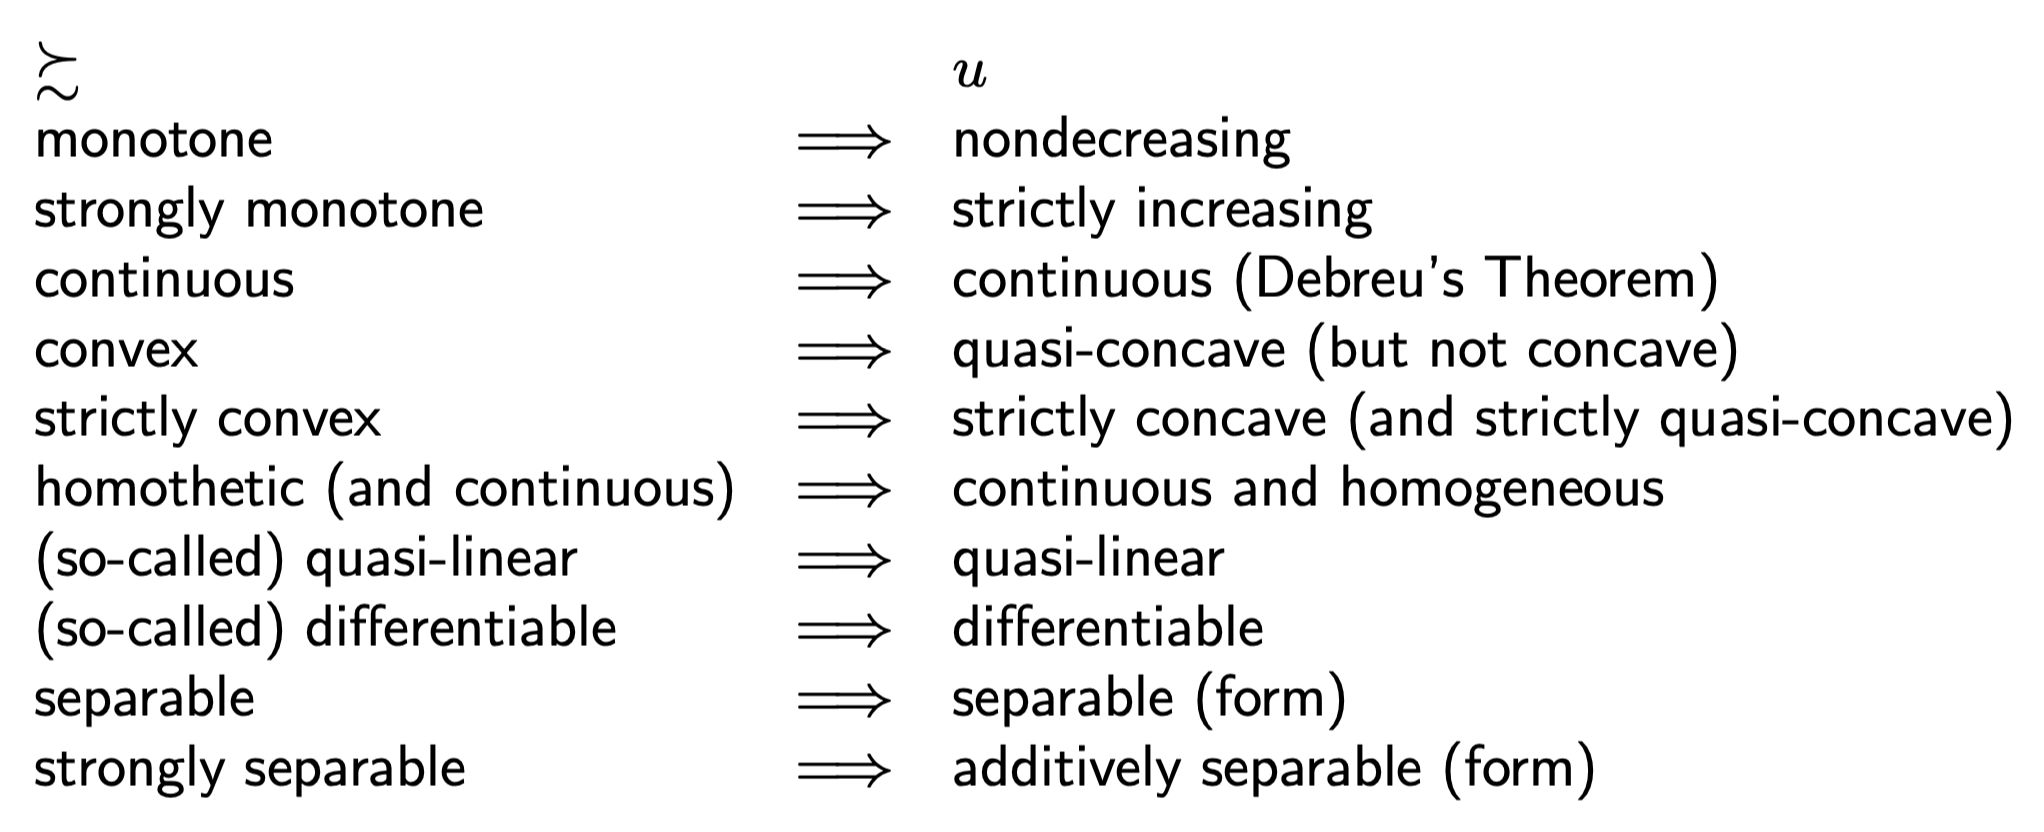
\includegraphics[scale=0.2]{Pref_prop.png}
    \caption{Properties of Preference and Utility Function}
    \label{}
\end{figure}\end{center}


\subsection{Independence of Preference}
The 'standard' model of decisions under risk is based on von Neumann and Morgenstern Expected Utility (EU), which requires the independence assumption.
\begin{definition}[Independence of Preference]
    \normalfont
    \textbf{Independence}: For any $x,y,z\in X$ and $0<\alpha<1$, if $x\succeq y$ then $\alpha x+(1-\alpha)z \succeq \alpha y+(1-\alpha)z$.
\end{definition}



\subsection{Continuous Preference}
\begin{definition}[Continuous $\succeq$]
    \normalfont
    $\succeq$ is \textbf{continuous} on $X$ \underline{if and only if} for any sequence $\{x^n,y^n\}_{n=1}^\infty$ with $x^n\succeq y^n$ and we note $x=\lim_{n \rightarrow \infty}x^n$, $y=\lim_{n \rightarrow \infty}y^n$, we have $x\succeq y$ (i.e., the graph $\{(x,y)\mid x\succeq y\subseteq X\times X\}$ is closed).
\end{definition}
\begin{proposition}[Debreu's Theorem, Continuous $\succeq$ $\Rightarrow$ continuous $u(\cdot)$]
    If $\succeq$ is continuous (on $X$, a convex subset of $\mathbb{R}^k$), then $\exists$ a continuous $u(\cdot)$ that represents $\succeq$.
\end{proposition}

\begin{example}[ (Lexicographic preferences (not continuous))]
    Under Lexicographic preference $\succ$, $x \succ y$ \underline{if and only if}
    \begin{enumerate}[$\circ$]
        \item $x_{1}>y_{1}$, or
        \item $x_{1}=y_{1}$, and $x_{2}>y_{2}$, or
        \item $x_{1}=y_{1}$ and $x_{2}=y_{2}$ and $x_{3}>y_{3}$, or
        \item etc.
    \end{enumerate}
    Under Lexicographic preferences, there is no indifference.
    
    We can find the Lexicographic preference violates continuity: $\left(1+\frac{1}{n}, 1\right) \succ(1,2)$ and $\lim \left(1+\frac{1}{n}, 1\right)=(1,1) \prec(1,2)$.
\end{example}

\begin{example}[ (Utility Representation for Lexicographic Preferences)]
    Consider the lexicographic preference $\succeq$ over the restricted domain $X=\left(\mathbb{Q}\cap[0,1]\right)\times [0,1]$. Enumerate the rationals in $[0,1]$ as $\mathbb{Q}\cap[0,1]=\{q^1,q^2,q^3,...\}$ where $q^i\neq q^j$ if $i\neq j$. The utility representation of this preference is
    $$u(x_1,x_2)=\sum_{q^i<q^j}\frac{1}{2^i}+\frac{1}{2^j}x_2, \textnormal{ where }q^j=x_1$$
\end{example}




\subsection{Homothetic Preference}
\begin{definition}[Homotheticity]
    \normalfont
    $\succeq$ are homothetic if $x\succeq y \Rightarrow \alpha x\succeq \alpha y$ for all $\alpha>0$.
\end{definition}

\begin{proposition}[Homothetic preference $\Leftrightarrow$ homogeneous $u(\cdot)$]
    A continuous $\succeq$ is homothetic $\Leftrightarrow$ $\exists$ a continuous homogeneous $u(\cdot)$ that represents $\succeq$ such that $u(\alpha x)=\alpha u(x)$ for all $x>0$.
\end{proposition}


\subsection{Quasi-linearity}
\begin{definition}[Quasi-Linearity]
    \normalfont
    $\succeq$ on $X$ is \textbf{quasi-linear} on $x_1$ if $$x\succeq y \Rightarrow (x+\epsilon e_1)\succeq (y+\epsilon e_1)$$ where $e_1=(1,0,...,0)$ and $\epsilon>0$.
\end{definition}

\begin{theorem}[Quasi-Linearity $\Leftrightarrow$ $u(x)=x_1+v(x_{-1})$]
    A continuous $\succeq$ on $(-\infty,\infty)\times \mathbb{R}_+^{K-1}$ is quasi-linear in $x_1$ $\Leftrightarrow$ $\exists$ a $u(\cdot)$ that represents $\succeq$ such that $$u(x)=x_1+v(x_{-1})$$
    where $v(\cdot)$ satisfies $(v(x_{-1}),0,...,0)\sim(0,x_{-1})$.
\end{theorem}

\subsection{Separability}
\begin{definition}[Separability]
    \normalfont
    $\succeq$ satisfies \textbf{separability} if for any $x_i$
    \begin{equation}
        \begin{aligned}
            (x_i, x_{-i})\succeq (x'_i, x_{-i}) \Leftrightarrow (x_i, x'_{-i})\succeq (x'_i, x'_{-i})
        \end{aligned}
        \nonumber
    \end{equation}
\end{definition}

\begin{theorem}[Separability $\Rightarrow$ Additive $u(\cdot)$]
    $\succeq$ with \textbf{separability} admits additive $u$-representation
    \begin{equation}
        \begin{aligned}
            u(x)=v_1(x_1)+\cdots v_K(x_K)
        \end{aligned}
        \nonumber
    \end{equation}
\end{theorem}

\begin{note}
    Strong assumption, usually ignored in practice.
\end{note}


\subsection{Differentiable Preference}
Consider a vector of values $v(x)\in \mathbb{R}^K_+$ for the $K$ commodities and a feasible the direction $x+\varepsilon d\in X$ from $x$ for small enough $\varepsilon>0$.

$d$ is considered \underline{improvement} if and only if $$d\cdot v(x)>0$$

Given $v(x): X \rightarrow \mathbb{R}^K_+$, let $$D_v(x)=\{d:d\cdot v(x)>0\}$$
be the set of directions that are improvements relative to $x$.

$d\in \mathbb{R}^k$ is an \underline{improvement direction} at $x$ if there is $\lambda^*>0$ such that $\lambda d$ is an improvement $$x+\lambda d\succ x$$
for any $\lambda\leq \lambda^*$. Let $D_{\succeq}(x)$ be the set of all improvement directions at $x$.

Any improvement is an improvement direction if
\begin{enumerate}[-]
    \item $\succeq$ are strictly convex.
    \item $\succeq$ are convex, strongly monotonic, and continuous.
\end{enumerate}

\begin{definition}[Differentiable Preference]
    \normalfont
    $\succeq$ is \textbf{differentiable} if there exists a function $v(x): X \rightarrow \mathbb{R}_+^K$ such that $$D_{\succeq}(x)=D_v(x),\ \forall x\in X$$
\end{definition}

\begin{example}
    $\succeq$ represented by
    \begin{enumerate}[(1).]
        \item $\alpha x_1+\beta x_2$ for $\alpha,\beta>0$ are differentiable: $v(x)=(\alpha,\beta)$.
        \item $\min\{\alpha x_1,\beta x_2\}$ are differentiable where $\alpha x_1\neq \beta x_2$: $v(x)=\left\{\begin{matrix}
            (1,0)& \textnormal{ if }\alpha x_1<\beta x_2\\
            (0,1)& \textnormal{ otherwise}
        \end{matrix}\right.$
    \end{enumerate}
\end{example}

\begin{proposition}[Sufficient condition for differentiable $\succeq$]
    Any (monotonic and convex) $\succeq$ can be represented by a (strongly monotonic and quasi-concave) and differentiable $u$ is differentiable.
\end{proposition}


\chapter{Choice Theory}
\section{Choice}
Let $\mathcal{B}=2^X$ (all subsets of $X$) and $B\in \mathcal{B}$ be the all potential alternatives that can be chosen.

The choice of an agent can be represented by $C(B)\subseteq B, \forall B\in \mathcal{B}$.

\begin{definition}[Choice Correspondence (More than one choice)]
    \normalfont
    A choice correspondence $C$ assigns a non-empty \underline{subset} for every non-empty set $A$
    $$\emptyset\neq C(A)\subseteq A$$
\end{definition}

\begin{definition}[Induced Choice Rule]
    \normalfont
    Given a binary relation $\succeq$, the \textbf{induced choice rule} $C_\succeq$ is defined by
    $C(A)=C_\succeq(A)=\{x\in A:x\succeq y, \forall y\in A\}, \forall A\subseteq X$.\\
    A choice function $c$ can be \textbf{rationalizable} if there is a preference relation $\succeq$ on $X$ such that $c=c_\succeq$.
\end{definition}

\begin{definition}[Revealed Preference]
    \normalfont
    Given a choice rule $\succeq$, its \textbf{revealed preference relation $\succeq_C$} is defined by $x \succeq_C y$ if there exists some $A$ such that $x, y \in A$ and $x \in C(A)$.
\end{definition}

\begin{proposition}
    If $C$ is rationalized by $\succeq$, then $\succeq=\succeq_C$.
\end{proposition}

\begin{definition}[Rubinstein's Condition $\alpha$]
    \normalfont
    A choice function $c$ satisfies \textbf{condition $\alpha$} if for any two problems $A,B$, if $A\subseteq B$ and $c(B)\in A$, then $c(A)=c(B)$.
\end{definition}
%Condition $\alpha$ is sufficient for $C$ is being formulated by maximizing a preference $\succeq$.

\subsection{Choice Function}
\begin{definition}[Choice Function]
    \normalfont
    A \textbf{choice function} $c$ such that $c(A)\in A$ which specifies a unique element for each nonempty subset $A\subseteq X$ (no indifferent preferences).
\end{definition}
\begin{proposition}[Rubinstein's Condition $\alpha$ $\Rightarrow$ Rationalizable Choice Function $c$]
    \begin{enumerate}[(1).]
        \item  Let $c$ be a choice function defined on a domain containing at least all subsets of $X$ of \underline{size of at most $3$}. If $c$ satisfies condition $\alpha$, then there is a preference $\succeq$ on $X$ such that $c=c_\succeq$.
        \item Let $c$ be a choice function with a domain $D$ satisfying that if \underline{$A, B \in D$, then $A \cup B \in D$}. If $c$ satisfies condition $\alpha$, then there is a preference relation $\succeq$ on $X$ such that $c = c_\succeq$.
    \end{enumerate}
\end{proposition}

\subsection{Choice Correspondence}
\begin{definition}[Sen's $\alpha$ or Independence of Irrelevant Alternatives]
    \normalfont
    If $a\in A\subseteq B$, then $a\in C(B) \Rightarrow a\in C(A)$.
\end{definition}

\begin{definition}[Sen's $\beta$]
    \normalfont
    If $a,b\in A\subseteq B$, then $a,b\in C(A)$ and $b\in C(B) \Rightarrow a\in C(B)$.
\end{definition}
$\alpha$ and $\beta$ are equivalent to WARP.
\begin{definition}[Weak Axiom of Revealed Preference (WARP)]\label{WARP}
    \normalfont
    Given a choice structure $(C,\mathcal{B})$ satisfies \textbf{WARP}. If $\exists B\in \mathcal{B}$ with $x,y\in B$, such that $x\in C(B)$. Then, $\forall B'\in \mathcal{B}$ with $x,y\in B'$, $y\in C(B') \Rightarrow x\in C(B')$.\\
    Or we can say, $$x,y\in B\cap B', x\in C(B), \textnormal{ and }y\in C(B') \Rightarrow x\in C(B')$$
\end{definition}

\begin{proposition}[Rational $\Rightarrow$ WARP]
    Given $\succeq$ is rational, then $(C^*_{\succeq},\mathcal{B})$ satisfies WARP.\\
    ($C^*_{\succeq}$ is the choice rule that picks the maximal alternatives by $\succeq$)
\end{proposition}

\begin{proposition}[Sen's Condition $\alpha,\beta$ $\Rightarrow$ Rationalizable Choice Correspondence $C$]
    Let $C$ be a choice correspondence defined on a domain containing at least all subsets of $X$ of \underline{size of at most $3$}. If $C$ satisfies condition $\alpha$ and $\beta$, then there is a preference $\succeq$ on $X$ such that $C=C_\succeq$.
\end{proposition}

\section{Revealed Preference}
Given choice data $(p^t,x^t)$, we say $u$-fucntion \underline{rationalizes} the observed behavior $(p^t,x^t)$ if for all $t=1,...,T$, $p^t x^t\geq p^t x \Rightarrow u(x^t)\geq u(x)$, that is, $u(\cdot)$ achieves its maximum value on the budget set at the chosen bundles.

If ``locally non-satiated'' $u$-function, $p^t x^t> p^t x \Rightarrow u(x^t)> u(x)$.

\begin{definition}[Revealed Preferred]
    \normalfont
    We say $x^t$ is
    \begin{enumerate}[-]
        \item $x^t R^D x$: \underline{\textbf{directly} revealed preferred} to $x$, if $p^t x^t \geq p^t x$; ($x$ is available under $p^t$)
        \item $x^t P^D x$: \underline{\textbf{strictly directly} revealed preferred} to $x$, if $p^t x^t > p^t x$;
        \item $x^t R x$: \underline{\textbf{indirectly} revealed preferred} to $x$, if $\exists$ a sequence $\{x_k\}_{k=1}^K$ with $x_1=x^t$ and $x_K=x$ such that $x_k R^D x_{k+1}$ for all $k=1,...,K-1$, i.e., $p^t x^t=p^t x_1\geq p^t x_2\geq ... \geq p^t x_K=p^t x$.
    \end{enumerate}
\end{definition}

\begin{definition}[Generalized Axiom of Revealed Preference (GARP)]
    \normalfont
    Consider two observations $(p^t,x^t)$ and $(p^s,x^s)$, GARP is satisfied if
    \begin{equation}
        \begin{aligned}
            x^t R x^s &\Rightarrow \textnormal{ not } x^s P^D x^t\\
            \textnormal{i.e., }x^t R x^s &\Rightarrow p^s x^t\geq p^s x^s
        \end{aligned}
        \nonumber
    \end{equation}
\end{definition}

GARP is a generalization of various other revealed preference tests
\begin{definition}
    \normalfont
    \underline{Weak Axiom of Revealed Preference (WARP)}:
    \begin{equation}
        \begin{aligned}
            x^t R^D x^s,x^t\neq x^s&\Rightarrow\textnormal{ not } x^s P^D x^t\\
            \textnormal{i.e., }p^t x^t \geq p^t x^s,x^t\neq x^s&\Rightarrow p^s x^t\geq p^s x^s
        \end{aligned}
        \nonumber
    \end{equation}
    \underline{Strong Axiom of Revealed Preference (SARP)}:
    \begin{equation}
        \begin{aligned}
            x^t R x^s,x^t\neq x^s&\Rightarrow\textnormal{ not } x^s R x^t
        \end{aligned}
        \nonumber
    \end{equation}
\end{definition}

\begin{theorem}[Afriat's Theorem]
    The following conditions are equivalent:
    \begin{enumerate}
        \item The data satisfies GARP;
        \item There exists a non-satiated $u$-function that rationalizes the data;
        \item There exists a concave, monotonic, continuous, non-satiated $u$-function that rationalizes the data.
        \item There exist positive numbers $(u^t,\lambda^t)$ for $t=1,...,T$ that satisfy the so-called Afriat inequalities: $$u^s\leq u^t+\lambda^t p^t(x^s-x^t),\ \forall t,s$$
    \end{enumerate}
\end{theorem}



\section{Choice under Uncertainty}
We want to model an uncertain prospect corresponding forms of function $u$.

The literature contains (basically) three sets of answers to these questions, differing in whether uncertainty is objective or subjective.

\begin{enumerate}[$\circ$]
    \item Objective uncertainty: von Neumann-Morgenstern (vNM).
    \item Subjective uncertainty: Savage.
    \item Horse lottery-roulette wheel theory: Anscombe and Aumann (A-A)
\end{enumerate}

\subsection{von Neumann-Morgenstern (vNM)}
The set of prizes is defined by $X$ and the set of probability measures (or distributions) over $X$ is denoted by $P$.
\underline{A compound lottery:} If $p,q\in P$ and $\alpha\in[0,1]$, then there is an element $\alpha p+(1-\alpha)q\in P$ which is defined by taking the convex combinations of the probabilities of each prize separately, or
$$(\alpha p+(1-\alpha)q)(x)=\alpha p(x)+(1-\alpha)q(x)$$
$(\alpha p+(1-\alpha)q)$ represents a compound lottery.

\begin{definition}[Three Axioms]
    \normalfont
    \textbf{\underline{Three Axioms}}
    \begin{enumerate}
        \item[(A1)] $\succ$ is a preference relation (asymmetric and negatively transitive);
        \item[(A2)] For all $p,q,r\in P$ and $\alpha\in[0,1]$, $p\succ q \Rightarrow \alpha p +(1-\alpha)r\succ \alpha q+(1-\alpha)r$.
        \item[(A3)] For all $p,q,r\in P$ such that $p\succ q\succ r$, $\exists \alpha,\beta\in (0,1)$ such that
        \begin{equation}
            \begin{aligned}
                \alpha p +(1-\alpha)r\succ q\succ \beta p +(1-\beta)r
            \end{aligned}
            \nonumber
        \end{equation}
    \end{enumerate}
\end{definition}
\begin{theorem}[vNM]
    $\succ$ on $P$ satisfies axioms (A1)-(A3) if and only if there exists a function $u:X \rightarrow \mathbb{R}$ such that
    \begin{equation}
        \begin{aligned}
            p\succ q \Leftrightarrow \sum_x p(x) u(x)>\sum_x q(x) u(x)
        \end{aligned}
        \tag{*}
        \label{*}
    \end{equation}
    Moreover, $u$ is unique up to a \underline{positive affine transformation}: there is another $u'$ represents $\succ$ in the sense of (\ref{*}) if and only if there exists $c>0$ and $d$ such that
    \begin{equation}
        \begin{aligned}
            u'(\cdot)=cu(\cdot)+d
        \end{aligned}
        \nonumber
    \end{equation}
\end{theorem}
\begin{remark}
    \begin{enumerate}[$\circ$]
        \item If $u$ represents $\succ$ then so will $v(\cdot)=f(u(\cdot))$ for any \textbf{strictly increasing} $f$.
        \item $k(p)=\sum_x p(x)u(x)$ gives an ordinal representation of $\succ$.
    \end{enumerate}
\end{remark}

\begin{lemma}[Four Lemmas obtained by the three axioms]
    If $\succ$ satisfies (A1) to (A3), then
    \begin{enumerate}[(L1).]
        \item If $p\succ q$ and $0\leq\alpha<\beta\leq 1$, then $$\beta p+(1-\beta)q\succ \alpha p+(1-\alpha)q$$
        \item If $p\succeq q\succeq r$ and $p\succ r$ $\Rightarrow$ there exists a unique $\alpha^*\in[0,1]$ such that $$q\sim \alpha^*p+(1-\alpha^*)r$$
        \item If $p\sim q$ and $\alpha\in[0,1]$ $\Rightarrow$ for all $r\in P$, $$\alpha p+(1-\alpha)r\succ \alpha q+(1-\alpha)r$$
        \item For any $x\in X$, let $\delta_x$ be the probability distribution degenerate at $x$, that is $\delta_x(x')=\left\{\begin{matrix}
            1,&\textnormal{ if }x'=x\\
            0,&\textnormal{ if }x'\neq x
        \end{matrix}\right.$ For all $p\in P$, we have $x_1,x_2\in X$ such that
        \begin{equation}
            \begin{aligned}
                \delta_{x_1}\succeq p\succeq \delta_{x_2}
            \end{aligned}
            \nonumber
        \end{equation}
    \end{enumerate}
\end{lemma}

\subsection{Savage (1954)}
Consider the situation that what the decision maker chooses depends critically on his/her subjectively assesses as the odds of the outcomes.

\underline{The basics of the Savage formulation:}
\begin{enumerate}[$\circ$]
    \item a set of $X$ of prizes/consequences;
    \item a set $S$ of the nature (states of the world).
\end{enumerate}
Each $s\in S$ is a compilation of all characteristics/factors about which the DM is uncertain and which are relevant to the consequences that will
result from her/his choice. The set $S$ is an exhaustive list of mutually exclusive states — only one
$s\in S$ will be the realized state.

We denote the choice space by $H$, as the set of all functions from $S$ to $X$ ($H=X^S$).

Savage seeks to find a subjective taste (the utility function) $u(\cdot)$ and a subjective belief (the probability measure) $\pi$ such that
\begin{equation}
    \begin{aligned}
        h\succ h' \Leftrightarrow \sum_{s\in S}\pi(s)u(h(s))>\sum_{s\in S}\pi(s)u(h'(s))
    \end{aligned}
    \nonumber
\end{equation}
Note that, it contains an assumption that $u(\cdot)$ is a function about $x$ which doesn't depend on the state of the world when it receives $x$.



\section{Social Choice}
Notations:
\begin{enumerate}
    \item We consider \underline{finite} set of alternatives $X$ and \underline{finite} set of agents $I$.
    \item We use $\mathcal{B}$ to denotes the set of all preference relations.
    \item We use $\mathcal{R}\subseteq \mathcal{B}$ to denotes the set of all rational preference relations.
    \item We use $\succeq\in \mathcal{R}$ to represents individual rational preference relation.
\end{enumerate}

\subsection{Social Welfare Function and Properties}
\begin{definition}[Social Welfare Function (SWF)]
    \normalfont
    A \textbf{social welfare function} (SWF) is a mapping $$f: \mathcal{A}\subseteq \mathcal{R}^I\rightarrow \mathcal{B}$$
    $\trianglerighteq=f(\succeq_1,...,\succeq_I)$ is interpreted as the \textbf{social preference relation}. It doesn't need to be rational (i.e., complete and transitive).
\end{definition}

\begin{definition}[SWF's Properties]\label{SWF_properties}
    \normalfont
    A social welfare function $f: \mathcal{A}\rightarrow \mathcal{B}$
    \begin{enumerate}[$\circ$]
        \item has \textbf{unrestricted domain} (UD) if $\mathcal{A}=\mathcal{R}^n$;
        \item is \textbf{transitive} (T) if $f(\succeq_1,...,\succeq_I)$ is transitive for all $(\succeq_1,...,\succeq_I)\in \mathcal{A}$;
        \item is \textbf{nondictatorial} (ND) if there is no agent $i\in I$ such that $\forall \{x,y\}\subseteq X$ $x\succeq_i y \Rightarrow x\trianglerighteq y$. (That is there is no distinguished voter who can choose the winner).
        \item is \textbf{weakly Paretian} (PA) if, $\forall \{x,y\}\subseteq X$ and any preference profile $(\succeq_1,...,\succeq_I)\in \mathcal{A}$, we have $x\succeq_i y,\forall i\in I \Rightarrow x\trianglerighteq y$.
        \item is \textbf{independent of irrelevant alternatives} (IIA) if, $\forall \{x,y\}\subseteq X$, and any $\succeq$ and $\succeq'$ with $\succeq_i\mid_{x,y}=\succeq'_i\mid_{x,y}, \forall i\in I$, if $x\trianglerighteq y$ then $x\trianglerighteq' y$.
    \end{enumerate}
\end{definition}


\subsection{Arrow's Theorem}
\begin{theorem}[Arrow's impossibility theorem]
    Suppose $|X|\geq 3$, $\mathcal{A}=\mathcal{R}^I$ (UD). Then if a SWF $f$ satisfies T, PA, and IIA, then it fails to be ND.
\end{theorem}
\begin{proof}
    \normalfont
    Yu, N. N. (2012). A one-shot proof of Arrow's impossibility theorem. \textit{Economic Theory}, 523-525.
\end{proof}



\chapter{Demand Theory}
\section{Utility Maximization Problem (UMP)}
Budget set is given by $B=\{x\in X\subseteq \mathbb{R}_+^K: p\cdot x\leq w\}$, where $w$ is the DM's wealth and $p$ is the vector of prices. Without losing generality, we can assume $w=1$.

The DM's problem is finding the $\succeq$-optimal bundle $x\in B(p)$. With the corresponding utility function $u(x)$, we can consider a consumer's problem
\begin{equation}
    \begin{aligned}
        \max_{x\in X} u(x)\\
        s.t.\ p\cdot x\leq w
    \end{aligned}
    \tag{UMP}
    \label{UMP}
\end{equation}
The set $\succeq$-optimal bundle is represented by $x(p,w)$.

\subsection{Marshallian Demand: Existence and Properties}

\begin{proposition}[Continuous Preference$\Rightarrow$ Solution $x(p,w)$ Existence]
    If $\succeq$ ($u(\cdot)$) is continuous, then all such problems have a solution $x(p,w)$.
\end{proposition}
\begin{proof}
    By the Weierstrass Extreme Value Theorem.
\end{proof}

\begin{proposition}[Convex Preference$\Rightarrow$ Convex $x(p,w)$]
    If $\succeq$ is convex ($u(\cdot)$ is quasi-concave), then $x(p,w)$ is convex.
\end{proposition}
\begin{proof}
    Suppose $x,x'\in X$. The optimal utility $u^*=u(x)=u(x')$. For any $\alpha\in[0,1]$, let $x''=\alpha x+(1-\alpha)x'$. Because $\succeq$ is convex, we have $u(\cdot)$ is quasi-concave, that is $u(x'')\geq u^*$. $x''$ is also feasible. So, $x''\in x(p,w)$.
\end{proof}

\begin{proposition}[Strictly Convex Preference$\Rightarrow$ Singleton $x(p,w)$]
    If $\succeq$ is strictly convex ($u(\cdot)$ is strictly quasi-concave), then $x(p,w)$ is (at most) a singleton.
\end{proposition}

\begin{proposition}[Differentiable Preference$\Rightarrow$ Margianl Utility equals to Price]
    If $\succeq$ is differentiable, $x^*\in x(p,w)$, and the vector of marginal values at $x^*$ (as defined above) is denoted by $v(x^*)=(v_1(x^*),...,v_K(x^*))$, where $v_k(x^*)$ is usually taken by $\frac{\partial u}{\partial x_k}(x^*)$ in "classic" problem. Then, we have
    \begin{equation}
        \begin{aligned}
            \frac{v_k(x^*)}{v_j(x^*)}=\frac{p_k}{p_j} \textnormal{ for any }x^*_k,x^*_j>0
        \end{aligned}
        \nonumber
    \end{equation}
    and for any $k$ with $x_k^*>0$ (consumed commodity)
    \begin{equation}
        \begin{aligned}
            \frac{v_k(x^*)}{p_k}\geq \frac{v_j(x^*)}{p_j}\textnormal{ for any }j\neq k
        \end{aligned}
        \tag{*}
        \label{*}
    \end{equation}
\end{proposition}

\begin{corollary}[Sufficient Conditions for Optimality]
    If $\succeq$ is strongly monotonic, convex, continuous, and differentiable and if $p\cdot x^*=w$ and \eqref{*} is satisfied then $x^*\in x(p,w)$
\end{corollary}

\begin{definition}[Rationalize]
    \normalfont
    $\succeq$ \textbf{fully rationalize} the demand function $x$ if for any $(p,w)$, the bundle $x(p,w)$ is the \underline{unique} $\succeq$-maximal bundle within $B$.\\
    A monotonic $\succeq$ \textbf{rationalize} the demand function $x$ if for any $(p,w)$, the bundle $x(p,w)$ is a $\succeq$-maximal bundle within $B$.
\end{definition}

The \underline{unique} solution is called Marshallian (Uncompensated) Demand.

\begin{proposition}[Properties of Marshallian Demand]
    \begin{enumerate}[(i).]
        \item \textbf{Walras' Law}: If $\succeq$ is local nonsatiation, $\forall x^*\in x(p,w): p\cdot x^*=w$.
        \item \textbf{Homogeneity of degree zero in $( p, w )$:} $x (\alpha p, \alpha w )\equiv x ( p, w ),\ \forall \alpha > 0$.
        \item \textbf{Continuous in prices and in wealth} if the $\succeq$ is continuous.
    \end{enumerate}
\end{proposition}


\begin{proposition}[Weak Axiom of Revealed Preference of Marshallian Demand]
    If demand is single valued then WARP(\ref{WARP}) is equivalent to $$p\cdot y'\leq w \textnormal{ and }y\neq y' \Rightarrow p'\cdot y>w$$
    where $y\equiv x(p,w)$ and $y'\equiv x(p',w')$.
    ($y'$ is feasible under $(p,w)$ but $y=x(p,w)$, which means $y$ is better and it can't be feasible under $(p',w')$.)
\end{proposition}

\subsection{Lagrangian Approach: $\frac{\partial u\left(x^{*}\right)}{\partial x_{i}}=\lambda^{*} p_{i}$ and $\lambda^*\left(x_i(p,w)+\sum_{j=1}^{K} p_{j} \frac{\partial x_{j}}{\partial p_{i}}\right)=0$}
The Lagrangian of the problem is $$L(x,\lambda)=u(x)-\lambda(p \cdot x-w)$$
By the KKT necessary conditions, we have
\begin{equation}
    \begin{aligned}
        \frac{\partial L}{\partial x_{i}}(x^*,\lambda^*)=\frac{\partial u\left(x^{*}\right)}{\partial x_{i}}-\lambda^{*} p_{i}=0,\ \forall i=1,...,K\\
        \lambda^*\geq 0 \textnormal{ and } \lambda^*(p\cdot x^*-w)=0
    \end{aligned}
    \nonumber
\end{equation}
Based on that, we have
\begin{lemma}
    \begin{enumerate}[(i).]
        \item $\frac{\partial u\left(x^{*}\right)}{\partial x_{i}}=\lambda^{*} p_{i}$;
        \item $\lambda^*\left(x(p,w)+p\cdot\frac{\partial x(p,w)}{\partial p}\right)=0$ i.e., $\lambda^*\left(x_i(p,w)+\sum_{j=1}^{K} p_{j} \frac{\partial x_{j}}{\partial p_{i}}\right)=0$.
    \end{enumerate}
\end{lemma}

\subsection{Envelope Theorem $\Rightarrow \lambda^{*}=\frac{\partial u(x(p, w))}{\partial w}$}
\begin{theorem}[Envelope Theorem]
    Consider the constrained maximization problem,
    \begin{equation}
        \begin{aligned}
            \max_{x\in \mathbb{R}^n}\quad & f(x;\theta)\\
            \textnormal{s.t. }& g(x;\theta)\leq 0
        \end{aligned}
        \nonumber
    \end{equation}
    where $xin \mathbb{R}^n$ is the choice variable and $\theta\in \mathbb{R}^m$ is some parameter. Let $f,g$ be continuously differentiable real-valued functions.
    \begin{enumerate}[$\bullet$]
        \item Let the value function of the problem be $V(\theta)\triangleq f(x^*(\theta),\theta)$.
        \item The Lagrangian for this problem is $$L(x,\lambda;\theta)=f(x; \theta)-\lambda g(x; \theta)$$
        \item Let $x^{*}$ and $\lambda^{*}$ denote the optimized values of the variables.
        \item[](By KKT necessary conditions, we have $\frac{\partial f}{\partial x}(x^*;\theta)=\lambda^* \frac{\partial g}{\partial x}(x^*;\theta)$ and $\lambda^* g(x^*;\theta)=0$)
    \end{enumerate}
    Then the following is true for any $\bar{\theta}\in \mathbb{R}^m$
    \begin{equation}
        \begin{aligned}
            \frac{\partial V}{\partial \theta_i}(\bar{\theta})=\frac{\partial L}{\partial \theta_i}(x^{*}, \lambda^{*};\bar{\theta})=\frac{\partial f}{\partial \theta_i}(x^{*};\bar{\theta})-\lambda^*\frac{\partial g}{\partial \theta_i}(x^{*};\bar{\theta})
        \end{aligned}
        \nonumber
    \end{equation}
\end{theorem}
\begin{proof}
    The proof of the envelope theorem is a straightforward calculation.\\
    Firstly, by KKT necessary conditions, we have $\frac{\partial f}{\partial x}(x^*;\bar{\theta})=\lambda^* \frac{\partial g}{\partial x}(x^*;\bar{\theta})$ and $\lambda^* g(x^*;\bar{\theta})=0 \Rightarrow \lambda^*\left[\frac{\partial g}{\partial x}(x^*;\bar{\theta})\frac{\partial x^*(\bar{\theta})}{\partial \theta_i}+\frac{\partial g}{\partial \theta_i}(x^*;\bar{\theta})\right]=0$. Then we have
    \begin{equation}
        \begin{aligned}
            \frac{\partial V}{\partial \theta_i}(\bar{\theta})&=\frac{\partial f}{\partial \theta_i}(x^*;\bar{\theta})+\frac{\partial f}{\partial x}(x^*;\bar{\theta})\frac{\partial x^*(\bar{\theta})}{\partial \theta_i}\\
            &\left(\textnormal{by }\frac{\partial f}{\partial x}(x^*;\bar{\theta})=\lambda^* \frac{\partial g}{\partial x}(x^*;\bar{\theta})\right)\\
            &=\frac{\partial f}{\partial \theta_i}(x^*;\bar{\theta})+\lambda^* \frac{\partial g}{\partial x}(x^*;\bar{\theta})\frac{\partial x^*(\bar{\theta})}{\partial \theta_i}\\
            &\left(\textnormal{by }\lambda^*\left[\frac{\partial g}{\partial x}(x^*;\bar{\theta})\frac{\partial x^*(\bar{\theta})}{\partial \theta_i}+\frac{\partial g}{\partial \theta_i}(x^*;\bar{\theta})\right]=0\right)\\
            &=\frac{\partial f}{\partial \theta_i}(x^{*};\bar{\theta})-\lambda^*\frac{\partial g}{\partial \theta_i}(x^{*};\bar{\theta})
        \end{aligned}
        \nonumber
    \end{equation}
\end{proof}

\begin{corollary}\label{corollary:marginal_wealth}
    $\lambda^{*}=\frac{\partial u(x(p, w))}{\partial w}$.
\end{corollary}
\begin{proof}
    By the envelope theorem, we have $\frac{\partial u(x(p, w))}{\partial w}=\left.\frac{\partial L}{\partial w}\right|_{x^{*}, \lambda^{*}}=\lambda^{*}$.
\end{proof}

\subsection{Indirect Utility Function $v(p, w) \equiv u(x(p, w))$}
\begin{proposition}[Properties of Indirect Utility Function]
    \begin{enumerate}
        \item $v(p,w)$ is homogeneous of degree zero in $(p, w)$;
        \item $v(p,w)$ is strictly increasing in $w$ and non-increasing in $p_{i}$;
        \item $v(p,w)$ is quasi-convex, that is the set $\{p:v(p,w)\leq u\}$ is convex for all $u\in \mathbb{R}$.
        \item $\lambda^{*}=\frac{\partial v(p, w)}{\partial w}$ (Corollary \ref{corollary:marginal_wealth}).
    \end{enumerate}
\end{proposition}

\subsection{Roy's Identity $x^*_i=-\frac{\frac{\partial v}{\partial p_{i}}}{\frac{\partial v}{\partial w}}$: recover $x(p, w)$ from $v(p, w)$}
\begin{proposition}[Roy's Identity]
    $x^*_i(p,w)=-\frac{\frac{\partial v(p,w)}{\partial p_{i}}}{\frac{\partial v(p,w)}{\partial w}}$.
\end{proposition}
\begin{proof}
    By the definition,
    \begin{equation}
        \begin{aligned}
            v(p, w) & \equiv u(x(p, w))&\\
            \frac{\partial v}{\partial p_{i}} & \equiv \sum_{j=1}^{K} \frac{\partial u}{\partial x_{j}} \frac{\partial x_{j}}{\partial p_{i}}&\\
            &=\sum_{j=1}^{K} \lambda^{*} p_{j} \frac{\partial x_{j}}{\partial p_{i}}& \textnormal{ by }\frac{\partial u\left(x^{*}\right)}{\partial x_{i}}=\lambda^{*} p_{i}\\
            &=-\lambda^{*} x_{i}^{*}&\textnormal{ by }\lambda^*\left(x_i(p,w)+\sum_{j=1}^{K} p_{j} \frac{\partial x_{j}}{\partial p_{i}}\right)=0\\
            x^*_i&=-\frac{\frac{\partial v}{\partial p_{i}}}{\frac{\partial v}{\partial w}}&\textnormal{ by }\lambda^{*}=\frac{\partial v(p, w)}{\partial w}
        \end{aligned}
        \nonumber
    \end{equation}
\end{proof}

\section{Expenditure Minimization Problem (EMP)}
Consider the duality
\begin{equation}
    \begin{aligned}
        \min_{x\in X}\quad & p\cdot x\\
        s.t.\quad & u(x)\geq u
    \end{aligned}
    \tag{EMP}
    \label{EMP}
\end{equation}
The optimal solutions are represented by $h(p,u)$. With uniqueness, we call it \textit{Hicksian (compensated) demand}.

\subsection{Hicksian Demand $h(p,u)$: Properties}
\begin{proposition}[Properties of Hicksian Demand]
    \begin{enumerate}[(i).]
        \item $h(p,u)$ is homogeneous of degree zero in $p$: $$h(tp,u)=h(p,u),\ \forall t\in \mathbb{R}_+$$
        \item $u ( x )$ is strictly quasi-concave $\Rightarrow$ $h ( p, u )$ is unique;
        \item For $u>u(0)$ and $u(\cdot)$ is locally non-satiated, \underline{constraint is active}: for all $x^*\in h(p,u)$, $$u(x^*)=u$$
    \end{enumerate}
\end{proposition}

\begin{lemma}[$\sum_{j=1}^{K} \frac{\partial u}{\partial x_j} \frac{\partial h_{j}}{\partial p_{i}}=0$]
    If $u ( x )$ is strictly quasi-concave, the Hicksian demand satisfies $\sum_{j=1}^{K} \frac{\partial u}{\partial x_j} \frac{\partial h_{j}}{\partial p_{i}}=0$
\end{lemma}
\begin{proof}
    $u(h(p,u))\equiv u \Rightarrow \sum_{j=1}^{K} \frac{\partial u}{\partial x_j}\frac{\partial h_{j}}{\partial p_{i}}=0$.
\end{proof}

\subsection{Expenditure Function $e(p,u)\equiv p\cdot h(p,u)$}
Given the Hicksian demand $h(p,u)$, we can define the expenditure function as $e(p,u)\equiv p\cdot h(p,u)$.
\begin{proposition}[Properties of Expenditure Function]\label{expen}
    \begin{enumerate}[(i).]
        \item $e ( p, u )$ is homogeneous of degree $1$ in $p$: $$e(tp,u)=tp\cdot h(tp,u)=tp\cdot h(p,u)=t e(p,u)$$
        \item $e ( p, u )$ is strictly increasing in $u$, non-decreasing in $p_i$;
        \item $e ( p, u )$ is \textbf{concave} in $p$;
        \item $e ( p, u )$ is continuous in $p$ for all $p>>0$;
        \item For all $x^*\in h(p,u)$, $x^*\in x(p,e(p,u))$;
        \item For $w>0$, $e(p,v(p,w))\equiv w$;
        \item $e(p,u)$'s derivative property: $$\frac{\partial e(p, u)}{\partial p_{i}} \equiv h_{i}(p, u)$$
    \end{enumerate}
\end{proposition}
\begin{proof}[Proof for concavity]
    Suppose the price of good 1 increases from $p_1^0$ to $p_1^1$: $p^0 \rightarrow	p^1$. Set $p^a=ap^0+(1-a)p^1,\ 0\leq a\leq 1$. So, $p^0\leq p^a\leq p^1$ and
    \begin{equation}
        \begin{aligned}
            e(p^a,u)&=p^a\cdot h(p^a,u)\\
            &=(ap^0+(1-a)p^1)\cdot h(p^a,u)\\
            &=a[p^0\cdot h(p^a,u)]+(1-a)[p^1\cdot h(p^a,u)]\\
            &h(p^a,u)\text{ is feasible in both EMP, but not optimal solutions}\\
            &\geq a[p^0\cdot h(p^0,u)]+(1-a)[p^1\cdot h(p^1,u)]\\
            &= ae(p^0,u)+(1-a)e(p^1,u)
        \end{aligned}
        \nonumber
    \end{equation}
\end{proof}

\begin{proof}[Proof for Derivative]
    \begin{enumerate}
        \item \underline{Direct proof:}
        $$
        \begin{aligned}
        e(p, u) & \equiv p \cdot h(p, u)& \\
        \frac{\partial e}{\partial p_{i}} & \equiv \sum_{j=1}^{K} p_{j} \frac{\partial h_{j}}{\partial p_{i}}+h_{i}& \\
        & \equiv \sum_{j=1}^{K} \frac{1}{\lambda^{*}} \frac{\partial u\left(x^{*}\right)}{\partial x_{j}} \frac{\partial h_{j}}{\partial p_{i}}+h_{i}& \textnormal{ by }\frac{\partial u\left(x^{*}\right)}{\partial x_{i}}=\lambda^{*} p_{i}\\
        &=h_i&\textnormal{ by }\sum_{j=1}^{K} \frac{\partial u}{\partial x_j} \frac{\partial h_{j}}{\partial p_{i}}=0
        \end{aligned}
        $$
        \item \underline{Envelope Theorem Proof:}
        \begin{equation}
            \begin{aligned}
                L(x,\lambda;(p,u))&=p\cdot x-\lambda (u(x)-u)\\
                \frac{\partial e(p,u)}{\partial p_i}&=\frac{\partial L(x,\lambda;(p,u))}{\partial p_i}\bigg|_{x^*=h(p,u)}=x_i|_{x^*=h(p,u)}=h_i(p,u)
            \end{aligned}
            \nonumber
        \end{equation}
    \end{enumerate}
\end{proof}

\subsection{Law of Compensated Demand: $\frac{\partial h_i}{\partial p_i}\leq 0$}
\begin{corollary}[Law of Compensated Demand]
    Hicksian demand is downward sloping in its own price, $$\frac{\partial h_i}{\partial p_i}\leq 0$$
\end{corollary}
\begin{proof}
    By the concavity of $e(p,u)$ (\ref{expen}), we can conclude $\nabla^2 e(p,u)\preceq 0$ (negative semi-definite). Then, we know its diagonal elements are non-positive $\frac{\partial e^2}{\partial^2 p_i}=\frac{\partial h_i}{\partial p_i}\leq 0$.
\end{proof}

\subsection{Shifts in Hicksian Demand: $\frac{\partial h_{i}}{\partial u}  \equiv \frac{\partial x_{i}}{\partial w} \frac{\partial e}{\partial u}$, same direction as $\frac{\partial x_{i}}{\partial w}$}
How does Hicksian demand curve shift when utility changes?
$$
\begin{aligned}
h_{i}(p, u) & \equiv x_{i}(p, e(p, u)) \\
\frac{\partial h_{i}}{\partial u} & \equiv \frac{\partial x_{i}}{\partial w} \frac{\partial e}{\partial u}
\end{aligned}
$$
We know $\frac{\partial e}{\partial u}>0$, so the direction of Hicksian demand shift is the same as $\frac{\partial x_{i}}{\partial w}$.\\
- Normal good: increasing utility shifts $h_{i}$ to the right.\\
- Inferior good: increasing utility shifts $h_{i}$ to the left.

\section{UMP and EMP}
\subsection{Slutsky Equation: substitution effect and income effect}
Slutsky: how change of $p_j$ (price in good $j$) affects $x_i$ (the demand of product $i$).
\begin{proposition}[Slutsky Equation]
    \begin{equation}
        \begin{aligned}
            \frac{\partial x_i(p,w)}{\partial p_j}=\underbrace{\frac{\partial h_i(p,u)}{\partial p_j}}_{\textnormal{substitution effect}}\underbrace{-\frac{\partial x_i(p,w)}{\partial w} x_j(p,w)}_{\textnormal{income effect}}
        \end{aligned}
        \nonumber
    \end{equation}
\end{proposition}
\begin{proof}
    \begin{equation}
        \begin{aligned}
            h_i(p,u)&\equiv x_i(p,e(p,u))\\
            \frac{\partial h_{i}}{\partial p_{j}} & \equiv \frac{\partial x_{i}}{\partial p_{j}}+\frac{\partial x_{i}}{\partial w} \frac{\partial e}{\partial p_{j}} \\
            & \equiv \frac{\partial x_{i}}{\partial p_{j}}+\frac{\partial x_{i}}{\partial w} h_{j}(p, u) \\
            & \equiv \frac{\partial x_{i}}{\partial p_{j}}+\frac{\partial x_{i}}{\partial w} x_{j}(p, e(p,u))
        \end{aligned}
        \nonumber
    \end{equation}
\end{proof}
\begin{enumerate}[$\circ$]
    \item \textbf{Substitution effect}: $\frac{\partial h_{i}}{\partial p_{j}}$, the change of relative prices change with constant utility will change the $x_i$.
    \item \textbf{Income (Wealth) effect}: $-\frac{\partial x_{i}}{\partial w} x_{j}(p, w)$, the change of price can be seen as change of wealth, which will also impact the $x_i$.
\end{enumerate}

\subsection{Relationship Between UMP and EMP}
\begin{figure}[htbp]
    \centering
    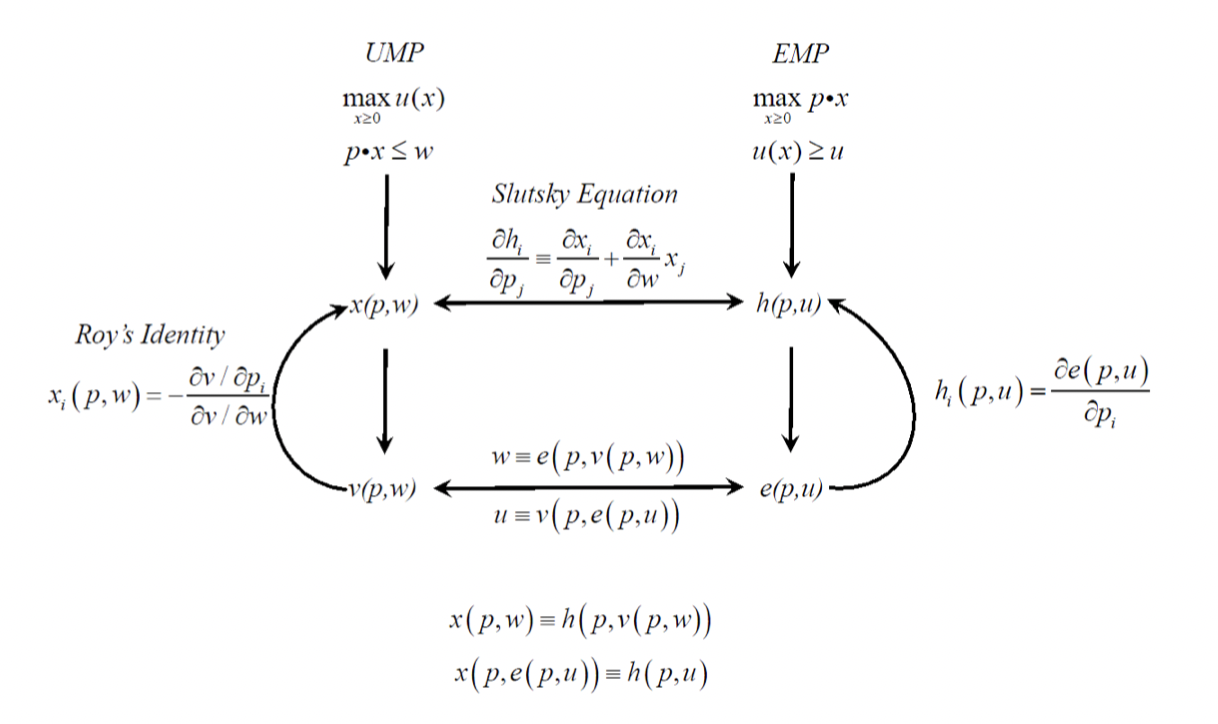
\includegraphics[scale=0.6]{UMP-EMP.png}
    \caption{Relationship Between UMP and EMP}
    \label{}
\end{figure}





















\chapter{General Equilibrium}
\section{Exchange Economy}
\begin{enumerate}
    \item There are $L$ perfectly divisible commodities indexed by $l=1,...,L$ over $\mathbb{R}^L$.
    \item There are $m$ agents, indexed by $i=1,...,m$. $N=\{1,...,m\}$.
    \item Each agent has a preference relation $\succeq_i$ on $\mathbb{R}_+^L$ represented by a utility function $u_i: \mathbb{R}_+^L \rightarrow \mathbb{R}$.
    \item Each agent has a vector of \underline{initial endowments} $w_i\in \mathbb{R}_+^L$.
    \item The \underline{aggregate endowment} is $w=\sum_{i=1}^m w_i$.
\end{enumerate}

\begin{example}[ (Endowment Box Economy)]
    The endowment box economy has $2$ goods ($L=2$) and 2 agents ($m=2$). The commodity space is $\mathbb{R}^2$.\\
    Each agent's consumption set is $\mathbb{R}_+^2=\{x\in \mathbb{R}^2:x\geq 0\}$.\\
    Each agent $i=a,b$ has preference relation $\succ_i$ over $\mathbb{R}_+^2$ represented by a utility function $u_i: \mathbb{R}_+^2 \rightarrow \mathbb{R}$.\\
    Each agent has a vector of initial endowments $w_i=(w_{i1},w_{i2})\in \mathbb{R}^2$.
\end{example}

\begin{definition}[Allocation]
    \normalfont
    An \textbf{allocation} in an exchange economy is an assignment of goods to agents $x=(x_1,...,x_m)\in \mathbb{R}_+^{L\times m}$ such that $\sum_{i=1}^mx_i=w$.
\end{definition}


\subsection{Pareto Optimal/Efficient}
\begin{definition}[Pareto Optimal]
    \normalfont
    An allocation $x$ is \textbf{Pareto optimal/efficient} if there doesn't exist an allocation $y$ s.t. $u_i(y_i)\geq u_i(x_i)$ ($y_i\succeq_i x_i$) for each $i$ and $u_j(y_j)> u_j(x_j)$ ($y_j\succ_j x_j$) for some $j$.
\end{definition}

Consider the following social planner's problem:
\begin{enumerate}[$\circ$]
    \item Fix an agent $j$ and $\{\bar{u}_i\}_{i\neq j}$,
    \begin{equation}
        \begin{aligned}
            \max_{(x_1,...,x_n)\in \mathbb{R}^{L\times m}_+} u_j(x_j)\\
            \textnormal{s.t. } u_i(x_i)\geq \bar{u}_i, i\neq j\\
            \sum_{i=1}^mx_i=w\\
            x_i\geq 0, \forall i
        \end{aligned}
        \tag{P}
        \label{Planner P}
    \end{equation}
\end{enumerate}

\begin{proposition}[P.O. $\Leftrightarrow$ Solutions of Problem (\ref{Planner P})]
    Suppose each agent's utility function is continuous and strongly monotone. Then, an allocation $x^*$ in an exchange economy is Pareto-Optimal \underline{iff} it is a solution of Problem (\ref{Planner P}) for some choice of $\{\bar{u}_i\}_{i\neq j}$.
\end{proposition}
\begin{proof}
    \begin{enumerate}
        \item ``$\Leftarrow$'': Suppose $x^*$ is a solution to Problem (\ref{Planner P}) for $\{\bar{u}_i\}_{i\neq j}$. Suppose by the way of contradiction that $x^*$ is not Pareto-Optimal. Then there is another allocation $\hat{x}$ such that
        \begin{enumerate}[(i).]
            \item Either: $u_j(\hat{x}_j)> u_j(x^*_j)$ and $u_i(\hat{x}_i)\geq u_i(x^*_i)$ for all $i\neq j$.
            \item Or: $u_j(\hat{x}_j)\geq u_j(x^*_j)$, $u_k(\hat{x}_k)\geq u_k(x^*_k)$ for some $k\neq j$, and $u_i(\hat{x}_i)\geq u_i(x^*_i)$ for all $i\neq j,k$.
        \end{enumerate}
        Suppose (i) holds: Since $\hat{x}$ is an allocation, $\sum_{i=1}^m \hat{x}_i = m$ and $\hat{x}_i\geq 0, \forall i$. By assumption and $x^*$ is solution of Problem (\ref{Planner P}), $u_i(\hat{x}_i)\geq u_i(x^*_i)\geq \bar{u}_i$ for all $i\neq j$. So, $\hat{x}$ satisfies the constraints of Problem (\ref{Planner P}). Because $u_j(\hat{x}_j)> u_j(x^*_j)$, $x^*$ is not the solution to Problem (\ref{Planner P}). Contradiction!\\
        Suppose (ii) holds: Prove by constructing another allocation $\tilde{x}$ as follows: By continuity, $\exists \epsilon>0$ sufficiently small s.t. $u_k((1-\epsilon)\hat{x}_k)\geq u_k(x^*_k)$. Set $\tilde{x}_k=(1-\epsilon)\hat{x}_k$, $\tilde{x}_j=\hat{x}_j+\epsilon \hat{x}_k$, and $\tilde{x}_i=\hat{x}_i$ for all $i\neq j,k$. Then, $\sum_{i=1}^m \tilde{x}_i=\sum_{i=1}^m \hat{x}_i=w$, $u_i(\tilde{x}_i)\geq u_i(x^*_i)\geq \bar{u}_i$ for all $i\neq j$ and $u_j(\tilde{x}_j)> u_j(x^*_j)\geq \bar{u}_j$ (by strong monotonicity). Hence, $x^*$ is not the solution to Problem (\ref{Planner P}). Contradiction!
        \item ``$\Rightarrow$'': Suppose $x^*$ is Pareto-Optimal. Set $\bar{u}_i=u_i(x^*)$ for all $i\neq j$.
        \begin{claim}
            $x^*$ solves Problem (\ref{Planner P}) given $\{\bar{u}_i\}_{i\neq j}$.
        \end{claim}
        Firstly, $x^*$ is feasible for Problem (\ref{Planner P}). Then, suppose by the way of contradiction that there is another allocation $x'$ such that $\sum_{i=1}^m x'_i=w$, $u_i(x'_i)\geq \bar{u}_i=u_i(x^*_i)$ for all $i\neq j$, and $u_j(x'_j)>u_j(x^*_j)$. Hence, $x^*$ is not Pareto-Optimal, which is a contradiction!
    \end{enumerate}
\end{proof}

\begin{proposition}
    From the first-order condition (FOC) of Problem (\ref{Planner P}), a \underline{necessary} condition for \underline{interior} Pareto-Optimal allocations when each $u_i$ is also differentiable is
    \begin{enumerate}[$\circ$]
        \item $Du_j(x^*_j)=\lambda_i Du_i(x^*_i)$ for some $\lambda_i>0$ and $\forall i\neq j$ where $x^*_i>>0, \forall i$.
    \end{enumerate}
\end{proposition}


\subsection{Individually Rational, Block, Core}
Are all Pareto-Optimal allocations equally likely are reasonable?

How the initial endowment allocation affects the Pareto-Optimal allocation?

One agent should block any proposed trades leading to allocations that generate lower utility.

\begin{definition}[Individually Rational]
    \normalfont
    A \underline{bundle} $x_i$ is \textbf{individually rational} (IR) for agent $i$ if $x_i\succeq_i w_i$.\\
    An \underline{allocation} $x=(x_1,...,x_m)$ is \textbf{individually rational} (IR) if $x_i\succeq_i w_i$ for all $i=1,...,m$.
\end{definition}

Let $N:=\{1,...,m\}$ be the set of agents. A \textbf{coalition} is a nonempty subset $S\subseteq N$.
\begin{example}
    With two agents $\{a,b\}$, there are 3 possible coalitions: $\{a\},\{b\},\{a,b\}$.
\end{example}

\begin{definition}[Block]
    \normalfont
    A coalition $S$ can \textbf{block} an allocation $x=(x_1,...,x_m)$ if there exists bundles $y_i\in \mathbb{R}^L_+$ for all $i\in S$ s.t.
    \begin{enumerate}[1.]
        \item $\sum_{i\in S}y_s=\sum_{i\in S}w_i$
        \item $y_i\succeq_i x_i$ for all $i\in S$;
        \item $y_j\succ_j x_j$ for some $j\in S$.
    \end{enumerate}
\end{definition}

\begin{definition}[Core]
    \normalfont
    The \textbf{core} is the \underline{set of allocations} that cannot be blocked by any coalition.
\end{definition}

\begin{note}(Core and P.O.)
    \begin{enumerate}[$\circ$]
        \item Every allocation in the core is Pareto-Optimal (directly by definition).
        \item Not every Pareto-Optimal allocation is in the core.
        \item For the \underline{two agent} case, the core is the set of individually rational Pareto-Optimal allocations.
    \end{enumerate}
\end{note}




\subsection{Competitive Equilibrium}
\begin{assumption}
    \normalfont
    Suppose there are markets for all available goods and all agents are \underline{price-takers} in these markets.
\end{assumption}
Given a vector of price $p\in \mathbb{R}^L$, agent $i$ chooses $x_i^*$ to solve the following problem:
\begin{equation}
    \begin{aligned}
        \max_{x_i\in \mathbb{R}^L_+}\ & u_i(x_i)\\
        s.t.\ & p\cdot x_i\leq p\cdot w_i
    \end{aligned}
    \nonumber
\end{equation}



\begin{definition}[Competitive Equilibrium]
    \normalfont
    Given endowment $w=(w_i)_{i\in N}$. A \textbf{competitive (Walrasian) equilibrium} in an exchange economy is a pair $p^*\in \mathbb{R}^L$ (price vector over $L$ goods) and an allocation $x^*=(x^*_i)_{i\in N}$ such that:
    \begin{enumerate}[(i).]
        \item $x_i^*\in \argmax u_i(x)$ s.t. $p^*\cdot x_i\leq p^*\cdot w_i, \forall i\in N$.
        \item $\sum_{i\in N}x_i^*=w$.
    \end{enumerate}
    We call $x^*=(x^*_i)_{i\in N}$ the \underline{competitive equilibrium (Walrasian) allocation}\\ and $p^*$ the \underline{competitive equilibrium (Walrasian) price vector}.
\end{definition}

Demand notations:
\begin{definition}[Excess Demand]
    \normalfont
    Let $x_i(p):=x_i(p,p\cdot w_i)$ denote agent $i$'s \textbf{demand} given the price vector $p\in \mathbb{R}^L$ and income $p\cdot w_i$.\\
    Agent $i's$ \textbf{individual excess demand at} $p$ is $x_i(p)-w_i$.\\
    The \textbf{aggregate excess demand} at $p$ is $\sum_{i\in N}x_i(p)-w$.
\end{definition}
\begin{note}(Excess Demand and Competitive Equilibrium)
    \begin{enumerate}[$\circ$]
        \item $p^*$ is a competitive equilibrium price vector \underline{if and only if} $0\in \sum_{i\in N}x_i(p)-w$
        \item $(x^*,p^*)$ is a competitive equilibrium \underline{if and only if} $x^*$ satisfies $x_i^*\in x_i(p^*), \forall i$ and $\sum_{i\in N}x^*_i-w=0$.
    \end{enumerate}
\end{note}











\subsection{First Welfare Theorem: CE $\Rightarrow$ P.O.}
Given non-satiated preference, every CE is P.O. (P.E.).
\begin{theorem}[First-order (fundamental) Welfare Theorem: CE $\Rightarrow$ P.O.]
    If each agent's preference relation is locally non-satiated, then every \underline{competitive equilibrium} allocation is \underline{Pareto optimal (Pareto efficient)}.
\end{theorem}
\begin{proof}
    Let $x^*=(x_1^*,...,x_n^*)$ be a CE allocation with corresponding CE price vector $p^*$.\\
    Suppose by way of contradiction that $x^*$ is \underline{not} P.O. allocation. Then, there is another allocation $\hat{x}=(\hat{x}_1,...\hat{x}_n)$ such that $\hat{x}_j\succ_j x^*_j$ for some $j\in N$ and $\hat{x}_i\succeq_i x^*_i$ for all $i\neq j$.\\
    By the definition of CE, $\hat{x}_j$ should not be affordable for $j$, i.e., $p^*\hat{x}_j>p^*w_j$. By the definitions of non-satiated and CE, $p^*\hat{x}_i\geq p^*w_i$ for all $i\neq j$. (If $p^*\hat{x}_i<p^*w_i$, $\exists \tilde{x}_i$ s.t. $p^*\tilde{x}_i\leq p^*w_i$ and $\tilde{x}_i\succ_i\hat{x}_i\succeq_i x_i^*$, which contradicts to the definition of CE.)\\
    Add up all inequalities, we get
    \begin{equation}
        \begin{aligned}
            p^*\cdot\left(\sum_{i=1}^n\hat{x}_i\right)> p^*\cdot\left(\sum_{i=1}^n w_i\right)=p^*\cdot w
        \end{aligned}
        \nonumber
    \end{equation}
    which contradicts to the definition of a feasible allocation that $\sum_{i}^n \hat{x}_i=w$. Hence, $x^*$ is P.O.
\end{proof}
\begin{note}
    This requires \textbf{only} \underline{local non-satiation} of preferences. In particular, does not require convexity of preferences.
\end{note}

\subsection{CE $\Rightarrow$ IR; CE $\subseteq$ P.O. $\cap$ Core}
\begin{note}[CE $\Rightarrow$ IR]
    At any prices $p$, an agent can always afford their initial endowment, so by revealed preference, every CE allocation is individually rational.
\end{note}
\begin{corollary}[CE Allocation is in Core]
    If each agent's preference relation is locally non-satiated, then every CE allocation is in the core.
\end{corollary}
\begin{proof}
    In exercise.
\end{proof}
\begin{note}
    Not every P.O. allocation is in the core. But every CE allocation is a P.O. allocation in the core.
    \begin{equation}
        \begin{aligned}
            \textnormal{CE}\subseteq \textnormal{P.O.}\cap \textnormal{Core}
        \end{aligned}
        \nonumber
    \end{equation}
\end{note}


\subsection{Equilibrium with Transfers}
What scope does planner have for redistribution using only decentralized market mechanism?

Not every P.O. allocation is ``equitable.'' To implement a more "equitable" allocation. Some possible mechanisms:
\begin{enumerate}[$\circ$]
    \item will need taxes or transfers (should be budget-balancing, i.e., no money leaves the economy).
    \item taxes/transfers should be lump-sum.
\end{enumerate}

\begin{definition}[``Supportable'' as a Price Equilibrium with Transfers]
\normalfont
    An \underline{allocation $x^*$} is \textbf{supportable} as a \textbf{price equilibrium with transfers} if there exists a price vector $p^*\in \mathbb{R}^L$ and lump-sum budget-balancing transfers $\{T_i:i=1,...,m\}$ so that $\sum_{i=1}^m T_i=0$, such that $\forall i$:
    \begin{equation}
        \begin{aligned}
            x_i^*\in \arg\max_{x\in \mathbb{R}^L_+ \textnormal{ s.t. } p^*\cdot x_i\leq p^*\cdot w_i + T_i}u_i(x_i)
        \end{aligned}
        \nonumber
    \end{equation}
\end{definition}


\subsection{Second Welfare Theorem: sufficient condition for P.O. be supported as a price equilibrium with transfers}
\begin{remark}
    Is every P.O. allocation supportable as a price equilibrium with transfers? \textbf{No.} (e.g. a non-convex indifference curve (preference relation): for a P.O. allocation, there exists an allocation such that gives a bundle with lower cost but equal utility for an agent.)
\end{remark}
Formally, a sufficient condition can be given:
\begin{theorem}[Second Welfare Theorem]\label{SWT_sup}
    If each consumers' preference relation is convex, continuous, and strongly monotone, then every interior P.O. allocation in an exchange economy can be supported as a price equilibrium with transfers.
\end{theorem}
To give the proof of the theorem, we need firstly give some definitions and results.
\begin{definition}[Supported by a price; Supported]
    \normalfont
    An allocation $\bar{x}=\left(\bar{x}_1,...,\bar{x}_m\right)$ in an exchange economy is \textbf{supported by a non-zero price vector $p\in \mathbb{R}^L$} if $$\forall i: x_i\succeq_i\bar{x}_i \Rightarrow p\cdot x_i\geq p\cdot\bar{x}_i$$
    If an allocation $\bar{x}=\left(\bar{x}_1,...,\bar{x}_m\right)$ is \textbf{supported}, then a \underline{common} price $p$ supports each agent's ``better-than set'' at $\bar{x}_i$ ($\{x_i\in \mathbb{R}_L^+: x_i\succeq_i\bar{x}_i\}$): $\forall x_i\in \{x_i\in \mathbb{R}_L^+: x_i\succeq_i\bar{x}_i\}: p\cdot x_i\geq p\cdot \bar{x}_i$.
\end{definition}
\begin{note}
    An allocation is supported as a price equilibrium with transfers $\Leftrightarrow$ the allocation that is supported (i.e., all agents' bundles are supported by a common price).
\end{note}

Recall:
\begin{theorem}[Separating Hyperplane Theorem]\label{SHT}
    Let $A,B\subseteq \mathbb{R}^n$ be non-empty disjoint, convex sets. Then $\exists p\in \mathbb{R}^n,p\neq 0$, s.t. $$p\cdot a\leq p\cdot b,\ \forall a\in A, \forall b\in B$$
\end{theorem}

\begin{proof}[Second Welfare Theorem \ref{SWT_sup}]
    Let $x^*=\left(x_1^*,...,x_m^*\right)$ be an interior P.O. allocation, so $x_i^*>>0, \forall i$. Let
    \begin{equation}
        \begin{aligned}
            P_i:=\left\{x_i\in \mathbb{R}_+^L:u_i(x_i)> u_i(x_i^*)\right\}, \ \forall i
        \end{aligned}
        \nonumber
    \end{equation}
    Properties about $P_i$:
    \begin{enumerate}[(1).]
        \item By strong monotonicity, $P_i\neq \emptyset$ (interior allocation) for all $i$.
        \item By convexity, $P_i$ is convex for all $i$.
    \end{enumerate}
    Let
    \begin{equation}
        \begin{aligned}
            P:&=P_1+\cdots+P_m\\
            &=\left\{z\in \mathbb{R}_L^+: z=\sum_{i=1}^m x_i \textnormal{ for some }(x_1,...,x_m)\in \mathbb{R}_+^{L\times m} \textnormal{ s.t. }u_i(x_i)> u_i(x_i^*), \forall i\right\}
        \end{aligned}
        \nonumber
    \end{equation}
    Properties about $P$:
    \begin{enumerate}[(1).]
        \item By construction, $P\neq \emptyset$.
        \item $P$ is convex: because the sum of convex sets is convex.
        \item $w\notin P$: this follows from the Pareto optimality of $x^*=\left(x_1^*,...,x_m^*\right)$.
    \end{enumerate}
    As $\{w\}$ is convex and $\{w\}\cap P=\emptyset$, by the Separating Hyperplane Theorem \ref{SHT}, $\exists p\in \mathbb{R}^L, p\neq 0$ s.t.  $p\cdot z\geq p\cdot w$ for all $z\in P$.
    \begin{enumerate}[$\circ$]
        \item
            \subitem Fix $j$ and suppose $u_j(x_j)>u_j(x_j^*)$ for some $x_j\in \mathbb{R}_+^L$. By continuity, $\exists \epsilon\in (0,1)$ sufficient small s.t. $u_j((1-\epsilon)x_j)>u_j(x_j^*)$. Let $y_j:=(1-\epsilon)x_j$. For $i\neq j$: set $y:=x_i^*+\frac{\epsilon}{m-1}x_j$. By strong monotonicity, $u_i(y_i)>u_i(x_i^*), \forall i\neq j$. So, $\sum_{i=1}^m y_i\in P$ by the definition of $P$.\\
            Then,
            \begin{equation}
                \begin{aligned}
                    p\cdot \left(\sum_{i=1}^m y_i\right)&\geq p\cdot w\\
                    \textnormal{By }\sum_{i=1}^m x_i^*=w,\quad p\cdot \left(\sum_{i=1}^m y_i-\sum_{i=1}^m x_i^*\right)&\geq 0\\
                    p\cdot \left(x_j-x_j^*\right)&\geq 0\\
                    p\cdot x_j&\geq p\cdot x_j^*
                \end{aligned}
                \nonumber
            \end{equation}
            That is, with $p$, $u_j(x_j)>u_j(x_j^*) \Rightarrow p\cdot x_j\geq p\cdot x_j^*$.
            \subitem
            By strong monotonicity, $u_j(x_j^*+(0,0,..,0,1,0,..,0))>u_j(x_j^*)$, hence, $p\cdot (x_j^*+(0,0,..,0,1,0,..,0))\geq p\cdot x_j^* \Rightarrow p\cdot (0,0,..,0,1,0,..,0)\geq 0$. That is, $p_i\geq 0,\forall i$. By definition, $p\neq 0$, $p>0$.\\
            By assumption $x_j^*>>0$, $p\cdot x_j^*>0$. Now suppose $\exists x_j\in \mathbb{R}_+^L$ s.t. $u_j(x_j)>u_j(x_j^*)$ and $p\cdot x_j=p\cdot x_j^*$. By continuity, $\exists\delta\in (0,1)$ s.t. $u_j(\delta x_j)>u_j(x_j^*)$. By what we show above, $u_j(x_j)>u_j(x_j^*) \Rightarrow p\cdot x_j\geq p\cdot x_j^*$. We have $p\cdot x_j>\delta p\cdot x_j=p\cdot (\delta x_j)\geq p\cdot x_j^*>0$. There is a contradiction. Hence, we prove that
            \begin{equation}
                \begin{aligned}
                    u_j(x_j)>u_j(x_j^*) \Rightarrow p\cdot x_j> p\cdot x_j^*
                \end{aligned}
                \nonumber
            \end{equation}
        \item Let the transfers be $T_i:=p\cdot x_i^*-p\cdot w_i, \forall i$ such that $\sum_{i}T_i=p\cdot (\sum_{i}x_i^*-\sum_{i}w_i)=0$.
    \end{enumerate}
    All in all,
    \begin{equation}
        \begin{aligned}
            x_i^*\in \arg\max_{x\in \mathbb{R}^L_+ \textnormal{ s.t. } p^*\cdot x_i\leq p^*\cdot w_i + T_i}u_i(x_i)
        \end{aligned}
        \nonumber
    \end{equation}
    $x^*$ is a price equilibrium with transfers $\{T_i\}_i$ and the price vector $p$.
\end{proof}

\subsection{Second Welfare Theorem: P.O. with Endowments Used $\Rightarrow$ CE}
\begin{theorem}[Second Welfare Theorem (corollary)]
    Suppose that interior $x^*$ is Pareto efficient and consumers receive endowment worth $p\cdot w^i=p\cdot {x^i}^*$ for all $i=1,...,m$. Then, if a competitive equilibrium exists for such $w$, then $x^*$ is a competitive equilibrium allocation.
\end{theorem}
\begin{proof}
    By the Second Welfare Theorem \ref{SWT_sup}, interior P.O. allocation $x^*$ can be supported by transfers $\{T_i\}_{i=1}^m$. Then, $p\cdot x_i\leq p\cdot w_i + T_i$. Because $p\cdot w^i=p\cdot {x^i}^*$, $T_i=0,\forall i$. So, $x^*$ is exactly a competitive equilibrium allocation.
\end{proof}

\subsection{Walras' Law in Competitive Equilibrium}
Recall that ``$p$ is a competitive equilibrium price vector'' $\Leftrightarrow$ ``$0\in \sum_{i=1}^m x_i(p)-w$.''

\begin{note}
Only relative prices matter, as the Marshallian demand has homogeneity of degree zero: $x(\lambda p)=x(p)$.
\end{note}

Hence, if $p^*$ is a competitive equilibrium price vector, so is $\lambda p^*, \forall \lambda$, which correspond to the same competitive equilibrium.

\begin{remark}
    \textbf{Are markets independent?} No.
\end{remark}

If $\succeq_i$ is locally non-satiated for all $i$, then $\forall i$: $p\cdot x_i(p)=p\cdot w_i, \forall p$. Adding over agents: $p\cdot \sum_{i=1}^mx_i(p)=p\cdot w, \forall p$.

This is \textbf{Walras' Law} in aggregate level: $p\cdot \left[\sum_{i=1}^mx_i(p)-w\right]=0, \forall p$.

\begin{remark}
    If Walras' Law holds and there exists $p^*>>0$ such that all markets but one clear, then the $p^*$ must clear the last market too.\\
    Let $Z(p)=\sum_{i=1}^mx_i(p)-w$. By Walras' Law, $p\cdot Z(p)=0, \forall p$. Suppose that exists $p^*>>0$ such that $Z_l(p^*)=0,l=1,...,L-1$. Then,
    \begin{equation}
        \begin{aligned}
            0=p^*\cdot Z(p^*)=\sum_{l=1}^Lp_l^*\cdot Z_l(p^*)=p^*_LZ_L(p^*)\\
            p_L^*>0 \Rightarrow Z_L(p^*)=0
        \end{aligned}
        \nonumber
    \end{equation}
\end{remark}

\section{Private Ownership Production Economy}
\begin{enumerate}
    \item There are $L$ perfectly divisible goods. The commodity space is $\mathbb{R}^L$.
    \item There are $m$ consumers. Each consumer $i=1,...,m$ has a preference relation $\succeq_i$ represented by a utility function $u_i: \mathbb{R}_+^L \rightarrow \mathbb{R}$, an initial endowment $w_i\in \mathbb{R}_+^L$, and owns shares $\{\theta_{ij}:j=1,...,J\}$ in the $J$ firms, where $\theta_{ij}\geq 0, \forall i,j$ and $\sum_{i=}^m\theta_{ij}=1, \forall j$.
    \item There are $J$ firms. Each firm $j=1,...,J$ has a production set $Y_j\subseteq \mathbb{R}^L$ that is nonempty, (representing the constraints of production).
    \begin{note}
        Standard sign convention regarding net output vectors: $y$ represents net output;\\
        $y_k\leq 0$ $\Rightarrow$ good $k$ is a net input in $y$;\\
        $y_k\geq 0$ $\Rightarrow$ good $k$ is a net output in $y$.
    \end{note}
    \item The set of allocation is
    \begin{equation}
        \begin{aligned}
            \mathcal{A}:=\left\{(x,y)=(\underbrace{x_1,...,x_m}_\textnormal{consumption},\underbrace{y_1,...,y_J}_\textnormal{production})\in \mathbb{R}^{L\times m}\times \mathbb{R}^{L\times J}: \sum_{i=1}^mx_i=\sum_{j=1}^J y_j+\sum_{i=1}^mw_i,y_j\in Y_j, \forall j\right\}
        \end{aligned}
        \tag{A}
        \label{A}
    \end{equation}
\end{enumerate}
Given $p\in \mathbb{R}^L$, firm $j$'s problem is to choose production plan $y_j^*$ s.t. $y_j^*\in y_j(p)=\arg\max p\cdot y_j$
\begin{equation}
    \begin{aligned}
        y_j^*\in y_j(p)=\arg\max_{y_j\in Y_j}\quad &p\cdot y_j
    \end{aligned}
    \tag{ystar}
    \label{eq:y_star}
\end{equation}

Given $p\in \mathbb{R}^L$ and production plans in $\{y_j(p),j=1,...,J\}$, consumer $i$'s problem is to choose $x_i^*$ s.t.
\begin{equation}
    \begin{aligned}
        x_i^*\in x_i(p)=\arg\max_{x_i\in \mathbb{R}^L_+}\quad& u_i(x_i)\\
        s.t.\quad& p\cdot x_i\leq p\cdot w_i+\sum_{j=1}^J\theta_{ij}p\cdot y_j(p)
    \end{aligned}
    \tag{xstar}
    \label{eq:x_star}
\end{equation}

\subsection{Competitive Equilibrium}
\begin{definition}[Competitive Equilibrium]
    \normalfont
    An allocation $(x^*,y^*)$ and a price vector $p^*\in \mathbb{R}^L$ are a \textit{competitive equilibrium} in a \underline{private ownership production economy} if
    \begin{enumerate}[(i).]
        \item $x_i^*\in x_i(p^*)$ (given by \eqref{eq:x_star}) for all agent $i$. That is,
        \begin{equation}
            \begin{aligned}
                x_i^*\in x_i(p^*)=\arg\max_{x_i\in \mathbb{R}^L_+}\quad& u_i(x_i)\\
        s.t.\quad& p^*\cdot x_i\leq p^*\cdot w_i+\sum_{j=1}^J\theta_{ij}p^*\cdot y^*_j(p^*)
            \end{aligned}
            \nonumber
        \end{equation}
        \item $y_j^*\in y_j(p^*)$ (given by \eqref{eq:y_star}) for all firm $j$. That is,
        \begin{equation}
            \begin{aligned}
                y_j^*\in y_j(p^*)=\arg\max_{y_j\in Y_j}\quad &p^*\cdot y_j
            \end{aligned}
            \nonumber
        \end{equation}
        \item Market clearing: $(x^*,y^*)\in \mathcal{A}$ (given by \eqref{A}). That is $$\sum_{i=1}^m x_i^*=\sum_{j=1}^J y_j^*+\sum_{i=1}^m w_i$$
    \end{enumerate}
\end{definition}

\begin{example}[ (Representative Agent Model)]
    There is a single consumer ($m=1$) and a single firm ($J=1$).\\
    For example, suppose there are $L=2$ goods: time (label/leisure) $x_l$ and consumption $x_c$.\\
    Suppose the firm's production set is defined by a production function $f: \mathbb{R}_+ \rightarrow \mathbb{R}$, so $$Y:=\{(-y_l,y_c)\in \mathbb{R}^2:y_l\geq 0,y_c\leq f(y_l)\}$$
    The set of feasible consumption bundles is
    \begin{equation}
        \begin{aligned}
            \Hat{Y}:=(\underbrace{Y+\{\omega\}}_{\{y+w:y\in Y\}})\cap \mathbb{R}_+^L
        \end{aligned}
        \nonumber
    \end{equation}
\end{example}

\subsection{Pareto Optimal}
\begin{definition}[Pareto Optimal]
    \normalfont
    An allocation $(x^*,y^*)$ in a private ownership production economy is \textbf{Pareto optimal} if there is no other allocation $(x,y)$ s.t. $x_i\succeq_i x_i^*, \forall i$ and $x_h\succ_h x_h^*$ for some $h$.
\end{definition}

\subsection{First-Welfare Theorem (production)}
\begin{theorem}[First-Welfare Theorem]
    If each consumer's preference relation is locally non-satiated, then every competitive equilibrium allocation in a private ownership production economy is Pareto optimal.
\end{theorem}
\begin{proof}
    Let $(x^*,y^*)$ be a competitive equilibrium allocation with corresponding equilibrium price vector $p^*$. Suppose by the way of contradiction that $(x,y)$ is not Pareto optimal. That is, $\exists$ an allocation $(x,y)$ s.t. $x_i\succeq_i x_i^*, \forall i$ and $x_h\succ_h x_h^*$ for some $h$. Then, by the \eqref{eq:x_star},
    \begin{equation}
        \begin{aligned}
            p^*\cdot x_h>p^*\cdot w_h+\sum_{j=1}^J\theta_{hj}p^*\cdot y_j^*
        \end{aligned}
        \nonumber
    \end{equation}
    and by local non-satiation,
    \begin{equation}
        \begin{aligned}
            p^*\cdot x_i\geq p^*\cdot w_i+\sum_{j=1}^J\theta_{ij}p^*\cdot y_j^*
        \end{aligned}
        \nonumber
    \end{equation}
    Adding together
    \begin{equation}
        \begin{aligned}
            \sum_{i=1}^m p^*\cdot x_i&>\sum_{i=1}^mp^*\cdot w_i+\sum_{j=1}^Jp^*\cdot y^*_j\\
            \Rightarrow \sum_{i=1}^m p^*\cdot x_i-\sum_{i=1}^mp^*\cdot w_i&=p^*\cdot\left[\sum_{i=1}^mx_i-\sum_{i=1}^mw_i\right]>\sum_{j=1}^Jp^*\cdot y^*_j
        \end{aligned}
        \nonumber
    \end{equation}
    As $\sum_{i=1}^m x_i=\sum_{j=1}^J y_j+\sum_{i=1}^m w_i$, we have $\sum_{i=1}^m x_i-\sum_{i=1}^m w_i=\sum_{j=1}^J y_j$,
    \begin{equation}
        \begin{aligned}
            \sum_{j=1}^Jp^*\cdot y_j=p^*\cdot\left[\sum_{i=1}^mx_i-\sum_{i=1}^mw_i\right]>\sum_{j=1}^Jp^*\cdot y^*_j
        \end{aligned}
        \nonumber
    \end{equation}
    There is a contradiction, since this implies there is a firm $j$ and $y_j\in Y_j$ s.t. $p^*\cdot y_j>p^*\cdot y^*_j$, which contradicts to the assumption that $y_j^*$ maximizes profits for form $j$ at $p^*$ (\eqref{eq:y_star}).
\end{proof}

\subsection{Equilibrium with Transfers}
\begin{definition}[``Supportable'' as a Price Equilibrium with Transfers]
\normalfont
    An \underline{allocation $(x^*,y^*)$} in a private ownership production economy is \textbf{supportable} as a \textbf{price equilibrium with transfers} if there exists a price vector $p^*\in \mathbb{R}^L$ and lump-sum budget-balancing transfers $\{T_i:i=1,...,m\}$ so that $\sum_{i=1}^m T_i=0$, such that:
    \begin{enumerate}
        \item $\forall i$,
        \begin{equation}
            \begin{aligned}
                x_i^*\in &\arg\max_{x\in \mathbb{R}^L_+}u_i(x_i)\\
                &\textnormal{ s.t. } p^*\cdot x_i\leq p^*\cdot w_i +\sum_{j=1}^J\theta_{ij}p^*\cdot y^*_j + T_i
            \end{aligned}
            \nonumber
        \end{equation}
        \item $\forall j$,
        \begin{equation}
            \begin{aligned}
                y_j^*\in \arg\max_{y_j\in Y_j}\ p^*\cdot y_j
            \end{aligned}
            \nonumber
        \end{equation}
        \item Feasibility: $$\sum_{i=1}^m x_i^*=\sum_{j=1}^J y_j^*+\sum_{i=1}^m w_i$$
    \end{enumerate}
\end{definition}

\subsection{Second Welfare Theorem (production)}
Production economy is a more general form of exchange economy. It is the same that not every P.O. allocation can be supported as a price signal with transfers.

\begin{theorem}[Second Welfare Theorem (production)]
    If each consumer's preference relation is continuous, strongly monotone, and convex, and each firm's production set is convex, then every interior P.O. allocation in a private ownership production economy can be supported as a price equilibrium with transfers.
\end{theorem}
\begin{proof}
    Let $(x^*,y^*)$ be an interior P.O. allocation, so $x_i^*>>0, \forall i$. The same as exchange economy, for each agent $i$, let $P_i:=\{x_i\in \mathbb{R}_+^L: u_i(x_i)>u_i(x_i^*)\}$ and let
    \begin{equation}
        \begin{aligned}
            P:&=P_1+\cdots+P_m\\
            &=\left\{z\in \mathbb{R}_L^+: z=\sum_{i=1}^m x_i \textnormal{ for some }(x_1,...,x_m)\in \mathbb{R}_+^{L\times m} \textnormal{ s.t. }u_i(x_i)> u_i(x_i^*), \forall i\right\}
        \end{aligned}
        \nonumber
    \end{equation}
    Then $P$ is non-empty and convex.

    In production side, let
    \begin{equation}
        \begin{aligned}
            Y:=\sum_{j=1}^JY_j=\left\{y\in \mathbb{R}^L:y=\sum_{j=1}^Jy_j \textnormal{ for some }(y_1,...,y_J) \textnormal{ s.t. }y_j\in Y_j, \forall j\right\}
        \end{aligned}
        \nonumber
    \end{equation}
    Then $Y+\{w\}$ is non-empty and convex.
    \begin{claim}
        $P\cap (Y+\{w\})=\emptyset$. This follows from the assumption that $(x^*,y^*)$ is P.O. (There is no allocation gives higher utilities while satisfies constraints).
    \end{claim}
    By the Separating Hyperplane Theorem \ref{SHT}, $\exists p\in \mathbb{R}^L, p\neq 0$, s.t.
    \begin{equation}
        \begin{aligned}
            p\cdot z\geq p\cdot(y+w), \forall z\in P \textnormal{ and } y\in Y
        \end{aligned}
        \tag{p:SHT}
        \label{SHTp}
    \end{equation}

    For each $i$, set $$T_i:=p\cdot x_i^*-p\cdot w_i-\sum_{j=1}^J\theta_{ij}p\cdot y_j^*$$
    Then,
    \begin{equation}
        \begin{aligned}
            p\cdot x_i^*=p\cdot w_i+\sum_{j=1}^J\theta_{ij}p\cdot y_j^*+T_i
        \end{aligned}
        \nonumber
    \end{equation}
    and
    \begin{equation}
        \begin{aligned}
            \sum_{1=1}^m T_i&=\sum_{i=1}^m \left(p\cdot x_i^*-p\cdot w_i-\sum_{j=1}^J\theta_{ij}p\cdot y_j^*\right)\\
            &=p\cdot \left(\sum_{i=1}^m x_i^*-\sum_{i=1}^m w_i-\sum_{j=1}^J y_j^*\right)\\
            &=p\cdot 0=0
        \end{aligned}
        \nonumber
    \end{equation}
    So, $\{T_i:i=1,...,m\}$ are budget balancing.
    \begin{claim}\label{C1}
        \begin{equation}
            \begin{aligned}
                p\cdot z\geq p\cdot (\sum_{i=1}^m x^*)=p\cdot (\sum_{j=1}^J y_j^*+\sum_{i=1}^m w_i)\geq p\cdot(y+w), \forall z\in P \textnormal{ and } y\in Y
            \end{aligned}
            \nonumber
        \end{equation}
    \end{claim}
    To prove this, first note the feasibility, $\sum_{j=1}^J y_j^*+\sum_{i=1}^m w_i\in Y+\{w\}$ and $\sum_{i=1}^m x_i^*=\sum_{j=1}^J y_j^*+\sum_{i=1}^m w_i$. By the \ref{SHTp},
    \begin{equation}
        \begin{aligned}
            p\cdot z\geq p\cdot\left(\sum_{j=1}^J y_j^*+\sum_{i=1}^m w_i\right)=p\cdot \left(\sum_{i=1}^mx_i^*\right), \forall z\in P
        \end{aligned}
        \nonumber
    \end{equation}
    Now using the strong monotonicity, for each $i$, we can choose a sequence $\{x_i^n\}\subseteq P_i$ s.t. $x_i^n \rightarrow x_i^*$ (e.g. $x_i^n=\left(1+\frac{1}{n}\right)x_i^*$). Let $z^n=\sum_{i=1}^m x_i^n$ for all $n$. Then, $z^n \in P$ for all $n$ and $z^n \rightarrow \sum_{i=1}^m x_i^*$.\\
    Let $y\in Y$ be arbitrary. By the \ref{SHTp},
    \begin{equation}
        \begin{aligned}
            &p\cdot z^n\geq p\cdot (y+w), \forall n\\
            \Rightarrow &\lim_{n \rightarrow \infty} p\cdot z^n=p\cdot\left(\sum_{i=1}^m x^*\right)\geq p\cdot (y+w)\\
            \Rightarrow & p\cdot\left(\sum_{j=1}^J y_j^*+\sum_{i=1}^m w_i\right)=p\cdot \left(\sum_{i=1}^mx_i^*\right)\geq p\cdot (y+w)
        \end{aligned}
        \nonumber
    \end{equation}
    That is, claim \ref{C1} is proved.
    \begin{claim}\label{C2}
        $\forall j$: $p\cdot y_j^*\geq p\cdot y_j, \forall y_j\in Y_j$
    \end{claim}
    To show this, we fix $k$ and $y_k\in Y_k$, such that $y_k+\sum_{j\neq k}y_j^*\in Y$. By claim \ref{C1},
    \begin{equation}
        \begin{aligned}
            &p\cdot (\sum_{j=1}^J y_j^*+w)\geq p\cdot \left(y_k+\sum_{j\neq k}y_j^*+w\right)\\
            \Rightarrow &p\cdot y_k^*\geq p\cdot y_k
        \end{aligned}
        \nonumber
    \end{equation}
    Hence, claim \ref{C2} is proved.
    \begin{claim}\label{C3}
        $\forall i$: $u_i(x_i)> u_i(x_i^*) \Rightarrow p\cdot x_i>p\cdot x_i^*$.
    \end{claim}
    Note that in the proof for the SWT in exchange economy, it is sufficient to show $\forall i$: $u_i(x_i)> u_i(x_i^*) \Rightarrow p\cdot x_i\geq p\cdot x_i^*$. Fix $h$ and let $x_h\in P_h$. So, $u_h(x_h)>u_h(x_h^*)$. By the continuity and strong monotonicity of preference, we have $x_h+\sum_{i\neq h}x_i^*\in P$ (we can increase each $x_i^*$ a little and reduce $x_h$). Hence, by \ref{C1},
    \begin{equation}
        \begin{aligned}
            &p\cdot (x_h+\sum_{i\neq h}x_i^*)\geq p\cdot \left(\sum_{i=1}^m x_i^*\right)\\
            \Rightarrow &p\cdot x_h\geq p\cdot x_h^*
        \end{aligned}
        \nonumber
    \end{equation}
    Hence, claim \ref{C3} is proved.

    All in all, SWT is proved.
\end{proof}


\section{Existence of Competitive Equilibrium}
\subsection{Excess Demand in Exchange Economies}
\begin{assumption}\label{C}
    Suppose
    \begin{itemize}
        \item each consumer's preference relation is continuous, strongly monotone, and strictly convex, and
        \item $\sum_{i}w_i>>0$.
    \end{itemize}
\end{assumption}
Based on this assumption \ref{C}, we have
\begin{enumerate}[$\circ$]
    \item Each agent's demand function $x_i:\mathbb{R}^L_{++} \rightarrow \mathbb{R}^L_+$ is well-defined, continuous, homogeneous of degree $0$, and satisfies Walras' Law (for individual).
    \item Excess demand function $Z:\mathbb{R}_{++} \rightarrow \mathbb{R}^L$ given by $$Z(p)=\sum_{i=1}^m x_i(p)-\sum_{i=1}^m w_i$$ is
    \begin{definition}[Condition (1) to (4)]
        \normalfont
        Given the Assumption \ref{C}, following conditions are satisfied:
        \begin{enumerate}[(1).]
            \item Continuous;
            \item Homogeneous of degree $0$;
            \item Satisfies Walras' Law: $p\cdot Z(p)=0, \forall p$;
            \item Bounded below: $\exists s>0$ s.t. $Z_l(p)\geq -s, \forall p, \forall l=1,...,L$.
        \end{enumerate}
    \end{definition}
\end{enumerate}

\subsection{Excess Demand in Production Economies}
We use the same assumption \ref{C} for consumers' preferences, and we add a assumption on the production side.
\begin{assumption}\label{F}
    Suppose each firm's production set $Y_j$ is
    \begin{itemize}
        \item closed,
        \item strictly convex ($y,y'\in Y_j \Rightarrow \alpha y+(1-\alpha)y'\in \textnormal{int}Y_j, \forall \alpha\in (0,1)$),
        \item bounded above ($\exists \bar{y}_j\in \mathbb{R}^L$ s.t. $y\leq \bar{y}_j, \forall y_j\in Y_j$), and
        \item $0\in Y_j$.
    \end{itemize}
\end{assumption}
Based on this assumption \ref{F}, we have
\begin{enumerate}[$\circ$]
    \item Each firm's supply function $y_j: \mathbb{R}_{++}^L \rightarrow \mathbb{R}^L$ is well-defined, continuous, and homogeneous of degree $0$.
\end{enumerate}
Based on assumption \ref{C} and \ref{F}, we have
\begin{enumerate}[$\circ$]
    \item Excess demand function $Z:\mathbb{R}_{++} \rightarrow \mathbb{R}^L$ given by $$Z(p)=\sum_{i=1}^m x_i(p)-\sum_{j=1}^Jy_j(p)-\sum_{i=1}^m w_i$$ is
    \begin{definition}[Condition (1) to (4)]
        \normalfont
        Given the Assumption \ref{F}, following conditions are satisfied:
        \begin{enumerate}[(1).]
            \item Continuous;
            \item Homogeneous of degree $0$;
            \item Satisfies Walras' Law: $p\cdot Z(p)=0, \forall p$;
            \item Bounded below: $\exists s>0$ s.t. $Z_l(p)\geq -s, \forall p, \forall l=1,...,L$.
        \end{enumerate}
    \end{definition}
    \item If $Z(p^*)=0$, then $p^*$ is a competitive equilibrium price vector, with corresponding equilibrium allocation $\left(x_1(p^*),...,x_m(p^*),y_1(p^*),...,y_J(p^*)\right)$.
\end{enumerate}

\subsection{Boundary Condition}
Since $Z$ is homogeneous of degree $0$, we can normalize prices, set
\begin{equation}
    \begin{aligned}
        \Delta:=\left\{p\in \mathbb{R}^L_+:\sum_{l=1}^Lp_l=1\right\}
    \end{aligned}
    \nonumber
\end{equation}
We give other notations:
\begin{equation}
    \begin{aligned}
        \partial\Delta:&=\left\{p\in \Delta: p_l=0 \textnormal{ for some }l\right\}\\
        \textnormal{int}\Delta:&=\left\{p\in \Delta: p_l>0, \forall l\right\}=\Delta\cap \mathbb{R}^L_{++}\\
    \end{aligned}
    \nonumber
\end{equation}

Consider an exchange economy. Let $p\in \partial \Delta$. Let $w_i>>0$. If $\succeq_i$ is strongly monotone on $\mathbb{R}^L_{++}$, then demand of agent $i$ is undefined at $p_i$ (infinity for the zero price good).

So, we add a condition for excess demand $Z$:
\begin{definition}[Condition (5)]
    \normalfont
    \begin{enumerate}
        \item[(5).] If $p^n\in \textnormal{int}\Delta, \forall n$ and $p^n \rightarrow p$, where $p\in \partial \Delta$, then $\max_l\{Z_l(p^n)\}\rightarrow +\infty$.
    \end{enumerate}
\end{definition}
\begin{note}
    \begin{enumerate}[-]
        \item Condition (5) holds in an exchange economy with assumption \ref{C};
        \item Condition (5) holds in a production economy with assumption \ref{C} and \ref{F};
        \item Condition (5) is \underline{not} true in general, and the condition (5) does \underline{not} imply $p^n_l \rightarrow 0 \Rightarrow Z_l(p^n) \rightarrow +\infty$ (relative prices matter!)
        \item By Walras' Law and lower bound on $Z$, then the converse holds:
        \begin{equation}
            \begin{aligned}
                Z_l(p^n)\rightarrow +\infty \Rightarrow p^n_l \rightarrow 0
            \end{aligned}
            \nonumber
        \end{equation}
    \end{enumerate}
\end{note}

So, if condition (1) to (5) hold and $p^n \rightarrow p$ where $p^n >>0$ and $p_l>0$, then $\{Z_l(p^n)\}$ is bounded.

\subsection{Existence of Competitive Equilibrium}
\begin{theorem}[Condition (1) to (5) $\Rightarrow$ $\exists$ a competitive equilibrium]
    Let $Z: \mathbb{R}^L_{++} \rightarrow \mathbb{R}^L$ be a function s.t. condition (1) to (5) are satisfied, that is
    \begin{enumerate}[(1).]
        \item Continuous;
        \item Homogeneous of degree $0$;
        \item Satisfies Walras' Law: $p\cdot Z(p)=0, \forall p$;
        \item Bounded below: $\exists s>0$ s.t. $Z_l(p)\geq -s, \forall p, \forall l=1,...,L$.
        \item If $p^n\in \textnormal{int}\Delta, \forall n$ and $p^n \rightarrow p$, where $p\in \partial \Delta$, then $\max_l\{Z_l(p^n)\}\rightarrow +\infty$.
    \end{enumerate}
    \begin{note}
        (Fulfilled when Assumption \ref{C} and \ref{F} are satisfied).
    \end{note}
    Then, $\exists \bar{p}\in \mathbb{R}^L_{++}$ s.t. $Z(\bar{p})=0$.
\end{theorem}
\begin{proof}
    First, restrict attention to $p\in\Delta=\left\{p\in \mathbb{R}^L_+:\sum_{l=1}^Lp_l=1\right\}$.
    \begin{enumerate}[$\circ$]
        \item For $p\in \textnormal{int}\Delta$, define a subset of good $\Lambda(p)\subseteq \{1,...,L\}$ by
        \begin{equation}
            \begin{aligned}
                \Lambda(p):=\left\{l\in \{1,...,L\}: Z_l(p)=\max_k Z_k(p)\right\}
            \end{aligned}
            \nonumber
        \end{equation}
        \item For $p\in \Delta\backslash\textnormal{int}\Delta=\partial \Delta$, let
        \begin{equation}
            \begin{aligned}
                \Lambda(p):=\left\{l\in \{1,...,L\}: p_l=0\right\}
            \end{aligned}
            \nonumber
        \end{equation}
    \end{enumerate}
    Then, note $\Lambda(p)\neq\emptyset, \forall p\in\Delta$.\\
    Define the correspondence $\varphi: \Delta \rightarrow 2^\Delta$ that maps a price vector $p$ to a set of prices by
    \begin{equation}
        \begin{aligned}
            \varphi(p):=\left\{q\in \Delta:q_l=0, \forall l\notin \Lambda(p)\right\}
        \end{aligned}
        \nonumber
    \end{equation}
    As $\Lambda(p)\neq\emptyset, \forall p\in\Delta$, we have $\varphi(p)\neq \emptyset$ for all $p$ and
    \begin{equation}
        \begin{aligned}
            \varphi(p):=\left\{\begin{matrix}
                \left\{q\in \Delta:q\in\arg\max_{\tilde{q}\in\Delta}\tilde{q}\cdot Z(p) \right\}& \textnormal{ if }p\in \textnormal{int}\Delta\\
                \{q\in\Delta:q\cdot p=0\}&\textnormal{ if }p\in \partial\Delta
            \end{matrix}\right.
        \end{aligned}
        \nonumber
    \end{equation}
    \begin{note}
        \begin{enumerate}
            \item $\varphi(p)\subseteq \partial \Delta \Leftrightarrow \Lambda(p)\neq\{1,...,L\}$
            \item $p\in\partial \Delta \Rightarrow p$ is not a fixed point of $\varphi$.
            \item $p$ is a fixed point of $\varphi$ $\Leftrightarrow$ $p\in \textnormal{int}\Delta$ and $\Lambda(p)=\{1,...,L\}$ $\Leftrightarrow$ $p\in \textnormal{int}\Delta$ and $\exists m\in \mathbb{R}$ s.t. $Z_l(p)=m, \forall l=\{1,...,L\}$.
            \item $p$ is a fixed point of $\varphi$ $\Leftrightarrow$ $p\in \textnormal{int}\Delta$ and $Z(p)=0$. (By Walras' Law: $0=p\cdot Z(p)=m \sum_{l}p_l=m$.)
            \item $Z(p)\neq 0$ $\Rightarrow$ $\Lambda(p)\neq\{1,...,L\}$ $\Rightarrow$ $\varphi(p)\subseteq \partial \Delta$.
        \end{enumerate}
    \end{note}
    Now it suffices to show $\varphi$ has a fixed point. Note that $\forall p\in \Delta$, $\varphi(p)$ is non-empty, convex, and compact, and $\Delta$ is non-empty, convex, and compact.
    \begin{claim}
        $\varphi$ has closed graph.
    \end{claim}
    Let $p^n \rightarrow p\in\Delta$ and $q^n \rightarrow q\in\Delta$ where $(p^n,q^n)\in$ graph $\varphi$ $\forall n$. We want to show $(p,q)\in$ graph $\varphi$ (i.e., $q\in \varphi(p)$):
    \begin{enumerate}[$\circ$]
        \item \underline{Case 1}: Suppose $p\in \textnormal{int}\Delta$. Since $p>>0$, assume without losing generality, $p^n>>0$ $\forall n$. Suppose $l\notin \Lambda(p)$, we must show $q_l=0$. Since $p>>0$, $l\notin \Lambda(p) \Rightarrow Z_l(p)<\max_{k}Z_k(p)$. Since $Z$ is continuous, $\exists N$, such that $\forall n\geq N$, $Z_l(p^n)<\max_k Z_k(p^n)$ $\Rightarrow l\notin \Lambda(p^n), \forall n\geq N$ $\Rightarrow q^n_l=0, \forall n\geq N$ $\Rightarrow q_l=\lim_{n \rightarrow \infty}q^n_l=0$. So, $q\in \varphi(p)$.
        \item \underline{Case 2}: Suppose $p\in \partial\Delta$. Without losing generality, we write $p=(0,...,0,p_{r+1},...,p_L)$, where $p_l>0$ for all $l=r+1,...,L$. So, $\Lambda(p)=\{1,...,r\}$ and $\varphi(p)=\{\tilde{q}\in\Delta:\tilde{q}_l=0,l=r+1,...,L\}$.
        \begin{enumerate}[-]
            \item \underline{Case 2A}: Suppose $\{p^n\}$ has a subsequence in $\textnormal{int}\Delta$. Without losing generality, let $\{p^n\}$ denote this subsequence. Since $p^n \rightarrow p\in\partial \Delta$, $\max_k Z_k(p^n) \rightarrow +\infty$. Also, by Walras' Law and lower bound in $Z$, $\{Z_l(p^n)\}$ is bounded for $l=r+1,...,L$.\\
            Since $p^n\in \textnormal{int}\Delta, \forall n$, $\exists N_2$ s.t. $\forall n\geq N_2$, $\Lambda(p^n)\subseteq \{1,...,r\}$. Since $q^n\in \varphi(p^n), \forall n$ and $q^n_l=0,\forall l=r+1,...,L, \forall n\geq N_2$, we have $q_l=\lim_n q_l^n=0$. Hence, $q\in \varphi(p)$.
            \item \underline{Case 2B}: No subsequence of $\{p^n\}$ lies in $\textnormal{int}\Delta$. Without losing generality, take $\{p^n\}\subseteq \partial \Delta$. Now, because $p_l>0$ for $l=r+1,...,L$, $\exists N_3$ s.t. $\forall n\geq N_3$, $p^n_l>0$ for $l=r+1,...,L$. Then, $\Lambda(p^n)\subseteq \{1,...,r\}, \forall n\geq N_3$.\\
            By the same argument above (in Case 2A), we have $q^n\in\varphi(p^n),\forall n$ $\Rightarrow$ $q^n_l=0,\forall l=r+1,...,L, \forall n\geq N_3$ $\Rightarrow$ $q_l=\lim_{n \rightarrow \infty}q_l^n=0, \forall l=r+1,...,L$. Hence, $q\in\varphi(p)$.
        \end{enumerate}
    \end{enumerate}
    All in all, $\varphi$ has closed graph. By Kakutani's Fixed Point Theorem, $\varphi$ has a fixed point. By above augment, $\bar{p}\in \textnormal{int}\Delta$ and $Z(\bar{p})=0$.
\end{proof}


\begin{corollary}
    If an exchange economy satisfies assumption \ref{C}, then it has a competitive equilibrium. If a private ownership production economy satisfies assumption \ref{C} and \ref{F}, then it also has a competitive equilibrium.
\end{corollary}


\section{Uniqueness of Equilibrium}
When is the equilibrium unique?

One condition:
\begin{definition}[Strong Weak Axiom]
    \normalfont
    The function $Z: \mathbb{R}_{++}^L \rightarrow \mathbb{R}^L$ satisfies the \underline{strong weak axiom} if for any $\bar{p}\in \mathbb{R}_{++}^L$ s.t. $Z(\bar{p})=0$ and any $p\in \mathbb{R}^L_{++}$ s.t. $p\neq \alpha\bar{p}, \forall \alpha>0$, $$\bar{p}\cdot Z(p)>0$$
\end{definition}

\begin{theorem}[Uniqueness of Equilibrium]
    If $Z: \mathbb{R}_{++}^L \rightarrow \mathbb{R}^L$ satisfies \underline{condition (1)-(5)} and \underline{strong weak axiom}, then there is a unique $p^*\in \textnormal{int}\Delta$ s.t. $Z(p^*)=0$.
\end{theorem}
\begin{proof}
    Since $Z$ satisfies condition (1)-(5), $\exists p^*\in \textnormal{int}\Delta$ s.t. $Z(p^*)=0$. By the strong weak axiom, if $p\in \textnormal{int}\Delta$ and $p\neq p^*$, then $p^*\cdot Z(p)>0$ $\Rightarrow$ $Z(p)\neq 0$. So, there is a unique $p^*\in \textnormal{int}\Delta$ s.t. $Z(p^*)=0$.
\end{proof}
\begin{example}
    \begin{enumerate}
        \item In an exchange economy with a representative consumer with strictly quasi-concave, strongly monotone, and $C^1$ (first-order continuously differentiable) utility function and $\omega>>0$, the excess demand function satisfies the strong weak axiom.
        \item If $Z$ satisfies \underline{gross substitutes} (for each $l$, $Z_l$ is increasing in $p_k,\forall k\neq l$), then $Z$ satisfies the strong weak axiom.
    \end{enumerate}
\end{example}


\section{Market Demand and Observable Implications}
Given an outcome, can we say it is obtained from an economy?

Restrict to exchange economies for simplicity.

\begin{theorem}[Sonnenschein-Mantel-Debreu (SMD) Theorem]
    Let $Z: \mathbb{R}_{++}^L \rightarrow \mathbb{R}^L$ be a function that is continuous and satisfies Walras' Law ($p\cdot Z(p)=0, \forall p$). Then $\forall \epsilon>0$ there is an exchange economy with $L$ consumers having continuous, strictly convex, strongly monotone preferences, and endowments $\{w_i:i=1,...,L\}\subseteq \mathbb{R}_+^L$, s.t., the excess demand function for this economy is equivalent to $Z$ on $\Delta^\epsilon=\{p\in\Delta: p_l\geq \epsilon, \forall l\}$.
\end{theorem}


\begin{theorem}[Mas-Colell Theorem]
    Let $E\subseteq \textnormal{int}\Delta$ be compact. Then there exists an exchange economy with $L$ consumers for which $E$ is the set of competitive equilibrium prices.
\end{theorem}

\begin{example}
    Suppose $L=2$, $Z: \mathbb{R}_{++}^2 \rightarrow \mathbb{R}^2$ satisfies condition (1)-(5). Choose good $2$ as numéraire, and set $p=(p_1,1)$. Then,
    \begin{enumerate}
        \item If $p_1$ is close to $0$, then $Z_1(p)>0$ by the boundary condition (5) and lower bound condition (4).
        \item If $p_1$ is large, then $Z_2(p)>0$ by the boundary condition (5) and lower bound condition (4). So, $Z_1(p)=-\frac{1}{p_1}Z_2(p)<0$ by Walras' Law (condition (3)).
        \item $\exists p_1^*$ s.t. $Z_1(p^*)=0$ by continuous $Z$ (condition (1)), and $p^*$ is an equilibrium price vector by Walras' Law (condition (3)).
    \end{enumerate}
\end{example}


\section{Comparative Statics and Local Uniqueness}
Restrict to exchange economies for simplicity.

Let $\vec{w}=(w_1,...,w_m)\in \mathbb{R}^{L\times m}_+$ denote profile of initial endowments.\\
Let $\mathcal{E}(\vec{w})$ denote the economy with fixed preference relations $\{\succeq_i:i=1,...,m\}$ and endowment profile $\vec{w}$.

Let $Z: \mathbb{R}_{++}^L\times \mathbb{R}_{++}^{L\times m} \rightarrow \mathbb{R}^L$ denote excess demand as a function of $(p,\vec{w})$, so
\begin{equation}
    \begin{aligned}
        Z(p,\vec{w}):= \sum_{i=1}^m x_i(p,p\cdot w_i)-\sum_{i=1}^m w_i
    \end{aligned}
    \nonumber
\end{equation}

Let
\begin{equation}
    \begin{aligned}
        Z_{-L}(p,\vec{w}):= \left(Z_1(p,\vec{w}),...,Z_{L-1}(p,\vec{w})\right)
    \end{aligned}
    \nonumber
\end{equation}
Normalize $p_L=1$. Given $\vec{w}$, equilibrium in $\mathcal{E}(\vec{w})$ corresponds to $p$ s.t. $Z_{-L}(p,\vec{w})=0$.

Assume $Z(\cdot,\vec{w})$ is $C^1$ and satisfies conditions (1)-(5), $ \forall \vec{w}$.

\begin{definition}[Regular Equilibrium]
    \normalfont
    Given $\vec{w}$, an equilibrium price vector $p$ is a \textbf{regular equilibrium} if $D_p Z_{-L}(p,\vec{w})$ is non-singular (has full rank $L-1$).
\end{definition}

\begin{definition}[Regular/Critical Economy]
    \normalfont
    If every equilibrium in the economy $\mathcal{E}(\vec{w})$ is regular, then $\mathcal{E}(\vec{w})$ is a \textbf{regular economy}. An economy that is not regular is a \textbf{critical economy}.
\end{definition}


\begin{proposition}
    \begin{enumerate}
        \item Regular equilibria are \underline{locally unique}.\\ ($\exists$ open set $V$ with $p^*\in V$ s.t. if $p\in V$, then $Z_{-L}(p,\vec{w})=0 \Leftrightarrow p=p^*$)
        \item A regular economy has \underline{finitely} many equilibria.
        \item In a regular economy, local equilibrium \underline{comparative statics} are determinate.
        \item $\mathcal{E}(\vec{w})$ is a regular economy if \underline{$0$ is a regular value} of $Z(\cdot,\vec{w})$. ($D_p Z(0,\vec{w})$ is non-singular).
    \end{enumerate}
\end{proposition}

\begin{theorem}[$C^1$ Demand Functions $\Rightarrow$ Regular Economy]
    Suppose each agent $i=1,...,m$ has a $C^1$ demand function: $x_i:\mathbb{R}_{++}^L\times \mathbb{R}_{++}^{L} \rightarrow \mathbb{R}_+^L$. Then almost all economy are regular. That is,
    \begin{equation}
        \begin{aligned}
            \left\{\vec{w}\in \mathbb{R}_{++}^{L\times m}: \mathcal{E}(\vec{w}) \textnormal{ is a critical economy}\right\}
        \end{aligned}
        \nonumber
    \end{equation}
    has Lebesgue measure zero in $\mathbb{R}^{L\times m}$.
\end{theorem}
\begin{proof}
    To prove $DZ_{-L}$ has full rank, it is sufficient to show the sub-matrix has rank $L-1$.
    
    Denote the derivative matrix of $DZ_{-L}(p,\vec{\omega})$ by $A$. The $(j,k)$ item of the matrix is
    \begin{equation}
        \begin{aligned}
            \frac{\partial x_{jk}}{\partial p_k}+\frac{\partial x_{jk}}{\partial w}\omega_k
        \end{aligned}
        \nonumber
    \end{equation}
    Compute the derivatives of $Z_{-L}$ with respect to the initial endowment of consumer $1$ ($\omega_1$). Denote the derivative matrix by $A$. The $(j,k)$ item of the matrix is
    \begin{equation}
        \begin{aligned}
            A_{jk}=\left\{\begin{matrix}
                \frac{\partial x_{1j}}{\partial w}(p,p\cdot\omega_1)p_k-1,&k=j\\
                \frac{\partial x_{1j}}{\partial w}(p,p\cdot\omega_1)p_k,&k\neq j
            \end{matrix}\right.
            ,j=1,...,L-1, k=1,...,L
        \end{aligned}
        \nonumber
    \end{equation}

    Minus $k=1,...,L-1$ column by $\frac{p_k}{p_L}$ times $L^\textnormal{th}$ column. We can get
    \begin{equation}
        \begin{aligned}
            \begin{bmatrix}
                    &A_{1L}\\
                -I_{L-1\times L-1}	&\vdots\\
                &A_{L-1,L}
            \end{bmatrix}
        \end{aligned}
        \nonumber
    \end{equation}
    which has rank $L-1$. Hence, $A$ has rank $L-1$.

    Hence, $0$ is a regular value of $Z_{-L}$. So, the result follows from the Transversality Theorem.
\end{proof}


\section{General Equilibrium with Uncertainty}
Set-up:
\begin{enumerate}
    \item There are $L$ (physical) goods.
    \item There are two time periods, $t=0,t=1$.
    \item At date $t=0$, the state of nature is determinate.
    \item At date $t=1$, there are $S$ ($s\in\{1,...,S\}$) possible states of nature, and all uncertainty resolves at $t=1$.
    \item Hence, the commodity space is $\mathbb{R}^{L\times(S+1)}$.
    \item Each consumer has preference relation $\succeq_i$ over $\mathbb{R}_+^{L\times(S+1)}$ represented by utility function $u_i$ and initial endowment under different states $w_i=(w_{i0},w_{i1},...,w_{iS})\in \mathbb{R}_+^{L\times(S+1)}$, where $w_{i0}$ is the endowment at $t=0$ and $w_{is}$ is the endowment at $t=1$ with state $s\in\{1,...,S\}$.
\end{enumerate}

\subsection{Basic Settings: (Complete) Contingent Commodities, Arrow-Debreu Equilibrium}
\begin{definition}[Contingent Commodity]
    \normalfont
    A unit of the \textbf{contingent commodity} (or \textbf{Arrow security}) $l_s$ is a claim to receive a unit of good $l$ \underline{if and only if} state $s$ occurs at date $t=1$
\end{definition}
Suppose at date $t=0$, there are markets for ``date $t=0$ consumption'' and ``a complete set of Arrow securities''.

Given price vector $p\in \mathbb{R}^{L\times (S+1)}$, agent $i$'s budget set is
\begin{equation}
    \begin{aligned}
        B_i(p)=\left\{x\in \mathbb{R}_+^{L\times(S+1)}: p\cdot x\leq p\cdot w_i\right\}
    \end{aligned}
    \nonumber
\end{equation}
\begin{definition}[Arrow-Debreu Equilibrium]
    \normalfont
    A competitive equilibrium in this model is an \textbf{Arrow-Debreu equilibrium}.
\end{definition}


\subsection{General: Asset Markets and Radner Equilibrium}
There is a market of spots. Assets are using for the trading across different stages.

\begin{note}
    \underline{Simplify:} assume all assets payoff in units of good $1$.
\end{note}

An asset is defined by its return vector $r\in\mathbb{R}^{S}$.

\begin{example}
    \begin{enumerate}
        \item Arrow securities $l_{\bar{s}}$ (for good $1$): $r_s=\left\{\begin{matrix}
            1,&s=\bar{s}\\
            0,&s\neq \bar{s}
        \end{matrix}\right.$
        \item Riskless bond: $r_s=1,\forall s$.
        \item Another asset: $r_s=\left\{\begin{matrix}
            1,& s \textnormal{ is even}\\
            -1,& s \textnormal{ is odd}
        \end{matrix}\right.$. Hence, $r=\left(-1,1,...,(-1)^{|S|}\right)$.
    \end{enumerate}
\end{example}

Suppose there are $K$ assets traded at date $t=0$, indexed by $k=1,...K$. Summarize their payoffs in an $S\times K$ matrix.
\begin{equation}
    \begin{aligned}
        R:=\begin{bmatrix}
            r_{11}&\cdots&r_{K1}\\
            \vdots&\vdots&\vdots\\
            r_{1S}&\cdots&r_{KS}\\
        \end{bmatrix}
    \end{aligned}
    \nonumber
\end{equation}
where $r_{ks}$ is the asset $k$'s return in state $s$.

Assume assets are in zero total supply. Let $z_i\in \mathbb{R}^k$ denote agent $i$'s portfolio. So,
\begin{equation}
    \begin{aligned}
        z_{ik}=\textnormal{\# units of asset $k$ bought/sold by agent $i$}
    \end{aligned}
    \nonumber
\end{equation}

Let $q=(q_1,...,q_K)\in \mathbb{R}^K$ denote the vector of asset prices.

Given an asset payoff structure $R$, the payoff from the portfolio $z_i$ is $Rz_i\in \mathbb{R}^S$.

Let $p_s\in \mathbb{R}^L$ denote price vector expected at date $0$ to hold in the spot market at date $t=1$ if state $s$ occurs.

\begin{definition}[Radner Equilibrium]
    \normalfont
    A consumption allocation $(x_1^*,...,x_m^*)$, portfolio profile $(z_1^*,...,z_m^*)$, spot price vectors $(p_0^*,p_1^*,...,p_S^*)$, and asset price vector $q^*$ are a \textbf{Radner equilibrium} if
    \begin{enumerate}
        \item For every agent $i$: $(x_i^*,z_i^*)$ solves
        \begin{equation}
            \begin{aligned}
                \max_{(x_i,z_i)\in \mathbb{R}^{L\times (S+1)}_+\times \mathbb{R}^K} &u_i(x_i)\\
                \textnormal{s.t. } &
                \left.\begin{matrix}
                p_0^*\cdot x_{i0}+q^*\cdot z_i\leq p_0^*\cdot w_{i0}\\
                p_s^*\cdot x_{is}\leq p_s^*\cdot w_{is}+p_{1s}^*(Rz_i)_s, \forall s
                \end{matrix}\right\}\triangleq B_i(p^*,q^*,R)
            \end{aligned}
            \nonumber
        \end{equation}
        (reminds that we assume all assets are payoff in good $1$).
        \item $\sum_{i=1}^mz_i^*=0$, $\sum_{i=1}^m x_i^*=\sum_{i=1}^m w_i$.
    \end{enumerate}
\end{definition}

\begin{note}
    \underline{Normalize:} $p_{1s}=1, \forall s=1,...,S$.
\end{note}
Then consumer $i$'s budget set is
\begin{equation}
    \begin{aligned}
        B_i(p,q,R):=\big\{x_i\in \mathbb{R}^{L\times (S+1)}_+:\exists z\in \mathbb{R}^K\textnormal{ s.t. }p_0\cdot x_{i0}+q\cdot z\leq p_0\cdot w_{i0}
        \textnormal{ and }p_s\cdot(x_{is}-w_{is})\leq (Rz_i)_s, \forall s\big\}
    \end{aligned}
    \nonumber
\end{equation}


\begin{definition}[Complete Asset Structure $R$]
    \normalfont
    The asset structure with return matrix $R$ is \textbf{complete} if $\textnormal{rank}R=S$. And the asset structure is \textbf{incomplete} if $\textnormal{rank}R<S$.
\end{definition}

\begin{theorem}[Arrow-Debreu Equilibrium $\Leftrightarrow$ Radner Equilibrium]
    Suppose preferences are \underline{strongly monotone} and the asset structure is \underline{complete}.
    \begin{enumerate}
        \item If $(x^*,p^*)$ is an Arrow-Debreu equilibrium, then there exists a portfolio profile $z^*$ and asset price vector $q^*$ such that $(x^*,p^*,q^*,z^*)$ is a Radner equilibrium.
        \item If $(x^*,p^*,q^*,z^*)$ is a Radner equilibrium, then there exists a vector $\mu\in \mathbb{R}_{++}^S$ (i.e., common beliefs) such that $(x^*,(p_0^*,\mu_1p_1^*,...,\mu_Sp_S^*))$ is an Arrow-Debreu equilibrium.
    \end{enumerate}
\end{theorem}



\begin{definition}[Arbitrage-free]
\normalfont
    For asset structure with return matrix $R$, the asset price vector $q\in \mathbb{R}^K$ is \textbf{arbitrage-free} if $\nexists z\in \mathbb{R}^K$ s.t. $q\cdot z\leq 0$ and $R z\geq 0$ with strict inequality for one.
\end{definition}

\begin{proposition}[Strongly Monotone $\Rightarrow$ Arbitrage-free]
    If preferences are strongly monotone, then in any Radner equilibrium, asset prices must be arbitrage-free.
\end{proposition}

We can also infer the components of assets from arbitrage-free prices.
\begin{theorem}[Reconstruct Assets from Arbitrage-free Prices]
    Consider an asset structure with return matrix $R$. If
    \begin{itemize}
        \item $q\in\mathbb{R}^K$ is arbitrage-free, \textbf{or}
        \item $q\in\mathbb{R}^K$ is a Radner equilibrium asset prices with $r_k\geq 0, r_k\neq 0, \forall k$.
    \end{itemize}
    then there exists $\mu\in \mathbb{R}_{++}^S$ such that $q=\mu^T R$, that is, s.t. $$q_k=\sum_s \mu_s r_{ks}, \forall k$$
\end{theorem}









\chapter{Game Theory}
Based on
\begin{enumerate}[$\circ$]
    \item "Kreps, D. M., \& Sobel, J. (1994). Signalling. \textit{Handbook of game theory with economic applications}, 2, 849-867."
    \item Mas-Colell, Whinston, and Green, Microeconomic Theory, Oxford University Press (1995).
    \item UIUC ECON 530 21Fall, Nolan H. Miller
    \item UC Berkeley ECON 201A 23Fall, 201B 24Spring
    \item UC Berkeley MATH 272 23Fall, Alexander Teytelboym
    \item  Jehle, G., Reny, P.: Advanced Microeconomic Theory. Pearson, 3rd ed. (2011). Ch. 6.
\end{enumerate}



\section{Basic Game Theory}
\subsection{Action and Domination Theorem}
Let $A$ be the finite set of possible actions and $\Omega$ be the finite set of possible states. A function can map the action and state to a value, $u(a,\omega)$. It can be represented by $\vec{u}(a)=\{u(a,\omega)\}_{\omega\in\Omega}$. It is common in game theory to assume the utility function is given or known.

A \textbf{mixed action} is a probability distribution over $A$, $\sigma\in\Delta(A)$.

A \textbf{belief} of the agent is a probability distribution over $\Omega$, $\mu\in\Delta(\Omega)$.

\begin{definition}[Optimal and Justifiable Mixed Action]
    \normalfont
    A mixed action $\sigma\in\Delta(A)$ is \textbf{optimal} given $\mu\in\Delta(\Omega)$ if $$\mathbb{E}_\mu u(\sigma,\tilde{\omega})\geq \mathbb{E}_\mu u(\sigma',\tilde{\omega}),\ \forall \sigma'\in \Delta(A)$$
    A mixed action $\sigma\in\Delta(A)$ is \textbf{justifiable} if it is optimal for some belief $\mu\in\Delta(\Omega)$.
\end{definition}

\begin{definition}[Dominant and Dominated Action]
    \normalfont
    A mixed action $\sigma\in\Delta(A)$ is \textbf{dominant} if $$u(\sigma,\omega)>u(\sigma',\omega),\ \forall \omega\in \Omega, \sigma'\in \Delta(A),\sigma\neq\sigma'$$
    A mixed action $\sigma\in\Delta(A)$ is \textbf{dominated} if $$u(\sigma,\omega)<u(\sigma',\omega),\ \forall \omega\in \Omega, \text{ and for some } \sigma'\in \Delta(A)$$
    In this case we say $\sigma'$ dominates $\sigma$.
\end{definition}

\begin{theorem}[Domination Theorem: Justifiable $=$ Not Dominated]
    A mixed action is justifiable \underline{if and only if} it is not dominated.
\end{theorem}
\begin{proof}
    $\Rightarrow$ is easily proved by the definition. We focus on proving $\Leftarrow$:
    
    Let $\mathcal{U}=\{\vec{u}(\sigma):\sigma\in\Delta(A)\}$ and $\sigma^*$ be an undominated mixed action. Then, we have $\mathcal{U}\cap(\{\vec{u}(\sigma^*)\}+\mathbb{R}_{++}^\Omega)=\emptyset$. Because $\mathcal{U}$ and $\{\vec{u}(\sigma^*)\}+\mathbb{R}_{++}^\Omega$ are disjoint, convex, and nonempty, we can use the Separating Hyperplane Theorem \ref{SHT}: $\exists p\in \mathbb{R}^\Omega,p\neq 0$ such that $p\cdot a\leq p\cdot b, \forall a\in\mathcal{U}, b\in (\{\vec{u}(\sigma^*)\}+\mathbb{R}_{++}^\Omega)$.

    \begin{claim}
        $p\cdot \vec{u}(\sigma)\leq p\cdot \vec{u}(\sigma^*), \forall \sigma\in\Delta(A)$.
    \end{claim}
    \begin{proof}
        For any positive number $m$, $\vec{u}(\sigma^*)+(\frac{1}{m},....,\frac{1}{m})\in \{\vec{u}(\sigma')\}+\mathbb{R}_{++}^\Omega$. So, for any $\sigma\in\Delta(A)$, $p\cdot \vec{u}(\sigma)\leq p\cdot\left(\vec{u}(\sigma^*)+(\frac{1}{m},....,\frac{1}{m})\right)$. By taking limit, $p\cdot \vec{u}(\sigma^*)=\lim_{m \rightarrow \infty}p\cdot\left(\vec{u}(\sigma^*)+(\frac{1}{m},....,\frac{1}{m})\right)\geq p\cdot \vec{u}(\sigma)$.
    \end{proof}
    \begin{claim}
        $p>0$.
    \end{claim}
    \begin{proof}
        Prove by the contradiction. Suppose $p_\omega<0$ for some $\omega\in\Omega$. Let $z=(\epsilon,...,\epsilon)+M\mathbb{1}_\omega, M>0,\epsilon>0$. So, $\vec{u}(\sigma^*)+z\in (\{\vec{u}(\sigma^*)\}+\mathbb{R}_{++}^\Omega)$. We have $p\cdot\vec{u}(\sigma^*)\leq p\cdot (\vec{u}(\sigma^*)+z)$ by the result of SHT. There is a contradiction since $p_\omega<0$. So, we have $p\geq 0$. Because $p\neq 0$, $p>0$ is proved.
    \end{proof}
    Finally, we normalize $p$ to $\mu=\frac{1}{\sum_{\omega}p_\omega}p$. Then, $\sigma^*$ is optimal for the belief $\mu$, which means $\sigma^*$ is justifiable.
\end{proof}










\subsection{Extensive Game}
\begin{definition}[History]
    \normalfont
    The sequences of actions are called \textbf{histories}. $h'=(\underbrace{a_1,...,a_n}_{h: \text{prefix of }h'},a_{n+1},...)\in H$. We call $h'$ is the \textbf{continuation} of $h$. $h$ is a \textbf{terminal} of $H$ if there is no continuation of $h$ in $H$. ($\emptyset\in H$.)
\end{definition}

\begin{definition}[Extensive Perfect Information Game]
    \normalfont
    Am extensive game with prefect information is defined as $G=\{N,A,H,Z,P,O,o,\succ_{n\in N}\}$, where $N$ is the set of players, $A$ is the set of actions, $H$ is the set of all histories, $Z$ is the set of all histories that are terminals, $P:H/Z \rightarrow N$ is a mapping from a non-terminal histories to a player (who moves after a non-terminal history), $O$ is the set of outcomes, and $o$ is a function from $Z$ to $O$.\\
    A PIG is \underline{finite horizon} if there is a bound on the length of its histories.
\end{definition}


We denote $A(h)$ as the actions available to player $P(h)$ after a history $h$.

Let $H_i=\{h\in H/Z:i=P(h)\}$ be the set of histories that player $i$ moves after.

\begin{definition}[Strategy]
    \normalfont
    A \textbf{strategy} is defined as a function $s_i:H_i \rightarrow A$ for which $s_i(h)\in A(h),\forall h\in H_i$. Let $S_i$ be the set of all strategies available to the player $i$. A \textbf{strategy profile} is a collection of strategy $s=(s_i)_{i\in N}$.
\end{definition}



\begin{definition}[Subgame]
\normalfont
    A \textbf{subgame} of a PIG $G=\{N,A,H,Z,P,O,o,\succ_{n\in N}\}$ is a game (a PIG) that starts after a given finite history $h\in H$. Formally, the subgame $G(h)$ associated with $h=(h_1,...,h_n)\in H$ is $G(h)=\{N,A,H_h,Z,P_h,O,o_h,\succ_{n\in N}\}$, where
    \begin{equation}
        \begin{aligned}
            H_h=\{(a_1,a_2,...):(h_1,...,h_n,a_1,a_2,...)\in H\}\\
            o_h(h')=o(hh'), P_h(h')=P(hh')
        \end{aligned}
        \nonumber
    \end{equation}
    A strategy $s$ of $G$ defines a strategy $s_h$ of $G(h)$ by $s_h(h')=s(hh')$.
\end{definition}

\begin{definition}[Subgame Perfect Equilibrium (SPNE)]
    \normalfont
    A \textbf{subgame perfect equilibrium (SPNE)} of $G$ is a strategy profile $s^*$ such that for every subgame $G(h)$ it holds that $h^{\prime} \mapsto s_i^*\left(h h^{\prime}\right)$ is an optimal strategy in $G(h)$, given beliefs that the rest of the players behave according to $s_{-i}^*$ (or its restriction to $G(h)$).
\end{definition}

\begin{definition}[Profitable Deviation]
    \normalfont
    Let $s$ be a strategy profile. We say that $s_i^{\prime}$ is a \textbf{profitable deviation} from $s$ for player $i$ at history $h$ if $s_i^{\prime}$ is a strategy for $G$ such that
    $$
    o_h\left(s_i^{\prime}, s_{-i}\right) \succ_i o_h(s)
    $$
\end{definition}
Note that a strategy profile has no profitable deviations iff it's a SPNE.

\begin{theorem}[The one-deviation principle]
    Let $G=\left(N, A, H, O, o, P,\left\{\preceq_i\right\}_{i \in N}\right)$ be a finite horizon, extensive form game with perfect information. Let $s$ be a strategy profile that is \underline{not} a subgame perfect equilibrium. There exists some history $h$ and a profitable deviation $\bar{s}_i$ for player $i=P(h)$ in $G(h)$ such that $\bar{s}_i(k)=s_i(k)$ for all $k \neq h$.
\end{theorem}
\begin{enumerate}[$\circ$]
    \item Let $G=\left(N, A, H, O, o, P,\left\{\preceq_i\right\}_{i \in N}\right)$ be a PIG.
    \item $A(\emptyset)$ is the set of allowed initial actions for player $i=P(\emptyset)$. For each $b \in A(\emptyset)$, let $s^{G(b)}$ be some strategy profile for the subgame $G(b)$.
    \item Given some $a \in A(\emptyset)$, we denote by $s^a$ the strategy profile for $G$ in which player $i=P(\emptyset)$ chooses the initial action $a$, and for each action $b \in A(\emptyset)$ the subgame $G(b)$ is played according to $s^{G(b)}$.
    \item So $s_i^a(\emptyset)=a$ and for every player $j, b \in A(\emptyset)$ and $b h \in H \backslash Z$, $s_j^a(b h)=s_j^{G(b)}(h)$.
\end{enumerate}
\begin{lemma}[Backward Induction]
    Let $G=\left(N, A, H, Z, O, o, P,\left\{\preceq_i\right\}_{i \in N}\right)$ be a finite PIG. Assume that for each $b \in A(\emptyset)$ the subgame $G(b)$ has a subgame perfect equilibrium $s^{G(b)}$. Let $i=P(\emptyset)$ and let $a$ be the $\succ_i$-maximizer over $A(\emptyset)$ of $o_a\left(s^{G(a)}\right)$. Then $s^a$ is a subgame perfect equilibrium of $G$.
\end{lemma}


\subsection{Strategic Form Game}
\begin{definition}[Normal Form Game]
    \normalfont
    A game in \textbf{normal form} is denoted by $$G =\left(\underbrace{N}_{\textnormal{players}},\underbrace{\{S_i\}_{i\in N}}_{\textnormal{Strategy Set}},\underbrace{\{u_i(\cdot)\}_{i\in N}}_{\textnormal{VNM utility}}\right)$$

    $u_i:\prod_{i\in I}S_i \rightarrow \mathbb{R}$ is the utility function that maps all players' strategies to a player's utilities.

    A \underline{finite} game is a normal-form game in which the set of players $N$ is a finite set, and the set of strategy profiles $S$ is finite.
\end{definition}

\begin{definition}[Mixed/Pure Strategy]
\normalfont
A mixed strategy  for player $i$ is a probability distribution $\sigma_i\in\Delta(S_i)$.\\
Elements of $S_i$ are called pure strategies.
\end{definition}

\begin{definition}[Dominant/Dominated Strategy]
    \normalfont
    A strategy $\sigma_i\in \Delta(S_i)$ is a \textbf{dominant strategy} for $i$ in $G$, if we have $u_i(\sigma_i,\sigma_{-i})> u_i(\sigma'_i,\sigma_{-i}), \forall \sigma'_i\neq \sigma_i, \sigma_{-i}\in\times_{j\neq i}\Delta(S_j)$.\\
    A strategy $\sigma_i\in \Delta(S_i)$ is a \textbf{dominated strategy} for $i$ in $G$, if $\exists \sigma'_i\neq \sigma_i$, $u_i(\sigma_i,\sigma_{-i})<u_i(\sigma'_i,\sigma_{-i}), \forall \sigma_{-i}\in\times_{j\neq i}\Delta(S_j)$.\\
    A strategy $\sigma_i\in \Delta(S_i)$ is a \textbf{weakly dominated strategy} for $i$ in $G$, if $\exists \sigma'_i\neq \sigma_i$, $u_i(\sigma_i,\sigma_{-i})\leq u_i(\sigma'_i,\sigma_{-i}), \forall \sigma_{-i}\in\times_{j\neq i}\Delta(S_j)$ and there is a $\sigma_{-i}\in \in\times_{j\neq i}\Delta(S_j)$, $u_i(\sigma_i,\sigma_{-i})< u_i(\sigma'_i,\sigma_{-i})$
\end{definition}

\begin{lemma}
    1. A dominant strategy is always pure.\\
    2. A strategy $\sigma'_i$ dominates $\sigma_i$ iff $u_i(\sigma'_i,s_{-i})> u_i(\sigma_i,s_{-i})$, for all pure strategy profiles $s_{-i}\in S_{-i}$.
\end{lemma}


\begin{definition}[Belief, Best Response]
    \normalfont
    A \textbf{belief} for player $i$ is a probability distribution $\mu\in\Delta(S_{-i})$.\\
    A strategy $\sigma_i \in \Delta(S_i)$ is the \textbf{best response} to beliefs $\mu$ if it solves the problem of $\max_{\sigma_i\in\Delta(S_i)}u_i(\sigma_i,s_{-i})$.\\
    Denote the set of all best responses to $\mu$ by $\beta_i(\mu)$.
\end{definition}
\begin{lemma}[Mixed Strategy is BR iff its Pure Strategies are Indifferent]
    A mixed strategy $\sigma_i$ is in $\beta_i(\mu)$ iff every pure strategy in the support of $\sigma_i$ is in $\beta_i(\mu)$. In particular, every strategy in the support of $\sigma_i$ yields the same payoff to $i$.
\end{lemma}

\begin{theorem}[Domination Theorem rephrased]
    In a finite game, a strategy is dominated iff there is no belief to which it is a best response.
\end{theorem}


\begin{definition}[Algorithm: Iterated Elimination of Dominated Strategies (IEDS)]
    \normalfont
    Let $\left(N,\left(S_i\right),\left(u_i\right)\right)$ be a finite game; $N=[n]$.
    \begin{enumerate}[$\bullet$]
        \item We define (inductively) $n$ sequences of sets of mixed strategies.
        \item Let $D_i^0=\Delta\left(S_i\right)$.
        \item Given $D_1^{k-1}, \ldots, D_n^{k-1}$, let
        $$
        D_i^k=\left\{\sigma_i: \nexists \bar{\sigma}_i: u_i\left(\sigma_i, \sigma_{-i}\right)<u_i\left(\bar{\sigma}_i, \sigma_{-i}\right) \forall \sigma_{-i} \in \times_{j \neq i} D_j^{k-1}\right\} .
        $$
        \item Note that $\left\{D_i^k\right\}$ is a decreasing sequence of sets.
        \item Let $D_i = \cap_{k=0}^\infty D_i^k$.
        \item The set $D = \times_{i=1}^n D_i$ be the set of strategies that survive the iterated elimination of dominated strategies.
    \end{enumerate}
    A game is called \textbf{dominance-solvable} if $D$ is a singleton.
\end{definition}


\begin{definition}[Rationalizable Strategies]
\normalfont
    \begin{enumerate}[$\bullet$]
        \item $R_i^0=\Delta\left(S_i\right)$.
        \item Given $R_1^{k-1}, \ldots, R_n^{k-1}$, Let
        $$
        \begin{aligned}
        & Z_i^k=\left\{s_i \in S_i: \sigma_i\left(s_i\right)>0 \text { for some } \sigma_i \in R_i^{k-1}\right\} \\
        & R_i^k=\left\{\sigma_i \in \Delta\left(S_i\right): \exists \mu \in \Delta\left(\times_{j \neq i} Z_j^k\right) \text { s.t. } \sigma_i \in \beta_i(\mu)\right\}
        \end{aligned}
        $$
    \end{enumerate}
    Note: $\left\{R_i^k\right\}_{k=0}^{\infty}$ is a decreasing sequence of sets.\\
    Let $R_i=\cap_{k=0}^{\infty} R_i^k$.\\
    The \textbf{rationalizable strategies} are the elements of $R=\times_{i=1}^n R_i$.
\end{definition}

\begin{lemma}
    In a finite game, $R$ is always non-empty and contains a pure strategy profile.
\end{lemma}

\begin{proposition}
    $\sigma_i \in \Delta(S_i)$ is \textbf{rationalizable} iff there are sets $Z_1,..., Z_n, Z_j \subseteq S_j$ such that
    \begin{enumerate}
        \item $\sigma_i \in \beta_i(\mu_i)$ for some $\mu_i \in \Delta(\times_{h\neq i}Z_h)$.
        \item for every $s_j \in Z_j$ there is $\mu_j \in \Delta(\times_{h\neq j}Z_h)$ such that $s_j\in \beta_j(\mu_j)$.
    \end{enumerate}
\end{proposition}

\begin{corollary}[Rationalizable = IEDS]
    Rationalizable strategies are exactly the strategies survive the iterated elimination of dominated strategies, $$R=D$$
\end{corollary}
















\subsection{Nash Equilibrium and Existence}
\begin{definition}[Nash Equilibrium]
    \normalfont
    A strategy profile $\Sigma=(\sigma_1,...,\sigma_I)$ is a \textbf{Nash} equilibrium of the game $G$ if for every $i\in I$, we have: $u_i(\sigma^*_i,\sigma^*_{-i})\geq u_i(\sigma'_i,\sigma^*_{-i}), \forall \sigma'_i\in \Delta(S_i)$ (no profitable deviation). In other words,
    \begin{enumerate}
        \item $\sigma_i$ is the \underline{best response} to beliefs $\mu_i\in \Delta (S_{-i})$
        \item $\mu_i=\sigma_{-i}$ (correct beliefs).
    \end{enumerate}
\end{definition}
\begin{enumerate}
    \item In rationalizable strategies, beliefs can be incorrect.
    \item In a Nash equilibrium, beliefs are correct. Any strategy in a Nash equilibrium is rationalizable.
\end{enumerate}

\begin{definition}[Best Response Correspondence]
    \normalfont
    In a Nash equilibrium the player $i$'s best response correspondence $\beta_i:\Delta(S_{-i})\rightarrow 2^{\Delta(S_i)}$ is defined as $\beta_i(\sigma_{-i})=\arg\max_{\sigma_i\in\Delta(S_i)}u_i(\sigma_i,\sigma_{-i})$. Let $\beta(\sigma)=\times_{i\in I}\beta_i(\sigma_{-i})$. Then $\sigma$ is a Nash equilibrium iff $\beta(\sigma)=\sigma$. $\beta$ is called the \textbf{best response correspondence} of the game.
\end{definition}

\begin{theorem}[Existence of Nash Equilibrium]
    A Nash equilibrium exists in a finite game $\Gamma$, if for all $i\in I$,
    \begin{enumerate}[(i).]
        \item $S_i$ is non-empty, convex, compact, subset of $\mathbb{R}^m$ (i.e., for some finite dimensions of real numbers).
        \item $u_i(s_i,...,s_I)$ is continuous in $(s_i,...,s_I)$ and quasi-concave in any $s_i$.
    \end{enumerate}
\end{theorem}
\begin{proof}
    We prove a lemma for the best response correspondence $\beta_i(s_{-i})=\argmax_{s_i\in S_i}u(s_i,s_{-i})$ firstly.
    \begin{lemma}
        Suppose $\{S_i\}_{i\in I}$ are non-empty. Suppose that $S_i$ is compact and convex and $u_i$ is continuous in $(s_i,...,s_I)$ and quasi-concave in any $s_i$, then best response correspondence $\beta_i(s_{-i})$ is non-empty, convex-valued and uhc.
    \end{lemma}
    \begin{proof}
        This lemma is proved by Berge's Maximum Theorem (Theroem \ref{thm:Berge's Maximum Theorem}).
    \end{proof}
    Consider the best response correspondence of the game $\beta$ with $\beta(s_i,...,s_I)=\{\beta_1(s_{-1}),...,\beta_I(s_{-I})\}$.

    As we proved $\beta$ is non-empty, convex-valued and uhc from $S$ to $S$ where $S$ is non-empty, compact, and convex. By the Kakutani's Fixed Point Theorem (Theorem \ref{thm:Kakutani's Fixed Point Theorem}), we have $\beta$ has a fixed point $s\in S$, which should be the Nash equilibrium.
\end{proof}

\subsection{Bayesian Game}
\begin{definition}[Bayesian Game]
    \normalfont
    A \textbf{Bayesian game} is defined by $$\Gamma=(I, \Omega, \{A_i\}_{i\in I}, \{u_i(\cdot)\}_{i\in I},\{\Theta_i\}_{i\in I}, \{F_i\}_{i\in I})$$
    where $\Omega$ is the state space, $u_i(a_i,a_{-i},\theta_i)$ maps the actions of players and player $i$'s type $\theta_i\in \Theta_i$ to player $i$'s utilities, and $F_i\in\Delta\left(\Omega\times\Theta_i\right)$ is the (prior) distribution of the player $i$'s type.
\end{definition}

\begin{definition}[Normal-form Bayesian game]
    \normalfont
    Assume a finite game. The \textbf{normal-form game} can be represented by $$\left(I,(S_i,U_i)_{i\in I}\right)$$ defined by letting $S_i$ be the set of strategies based on types $s_i:\Theta_i \rightarrow A_i$ and
    \begin{equation}
        \begin{aligned}
            U_i(s)=\sum_{\omega\in\Omega}\sum_{(\theta_i)_{i\in I}\in \Theta}p(\omega,\theta_1,...,\theta_I)u_i(s_1(\theta_1),..., s_I(\theta_I),\omega)
        \end{aligned}
        \nonumber
    \end{equation}
    for all $s\in S$.

    A \textbf{Bayesian Nash equilibrium} of a Bayesian game is a strategy profile $(s_1,...,s_n)$ that is a Nash equilibrium of the derived normal-form game.
\end{definition}

\begin{definition}[Best Response, Interim Payoff]
    \normalfont
    $s_i$ is a BR to $s_{-i}$ iff for all $\theta_i$, $s_i(\theta_i)$ maximizes the \textbf{interim payoff} of player $i$. The interim payoff is defined by the expected payoff given the type $\theta_i$ of player $i$ by playing action $a_i$.
    \begin{equation}
        \begin{aligned}
            \mathbb{E}_{\omega\in\Omega,\tilde{\theta}_{-i}\in\Theta_{-i}}[u_i(a_i,s_{-i}(\tilde{\theta}_{-i}),\omega)|\theta_i]
        \end{aligned}
        \nonumber
    \end{equation}
\end{definition}

\subsection{Zero-sum Game}
Consider a zero-sum game of two players, where player 1 moves firstly and player 2 moves secondly. The strategy of the player 1 is given by
\begin{equation}
    \begin{aligned}
        \max_{\sigma_1}\min_{\sigma_2}u(\sigma_1,\sigma_2)
    \end{aligned}
    \nonumber
\end{equation}
and the strategy of the player 2 is given by
\begin{equation}
    \begin{aligned}
        \min_{\sigma_2}\max_{\sigma_1}u(\sigma_1,\sigma_2)
    \end{aligned}
    \nonumber
\end{equation}
\begin{proposition}
    Move secondly is always better than move firstly. That is,
    \begin{equation}
        \begin{aligned}
            \max_{\sigma_1}\min_{\sigma_2}u(\sigma_1,\sigma_2)\leq \min_{\sigma_2}\max_{\sigma_1}u(\sigma_1,\sigma_2)
        \end{aligned}
        \nonumber
    \end{equation}
\end{proposition}
\begin{proof}
    As $u(\sigma_1',\sigma_2)\leq \max_{\sigma_1}u(\sigma_1,\sigma_2)$ for all $\sigma_1'$, we have
    \begin{equation}
        \begin{aligned}
            \min_{\sigma_2}u(\sigma_1',\sigma_2)&\leq \min_{\sigma_2}\max_{\sigma_1}u(\sigma_1,\sigma_2),\forall \sigma_1'\\
            \Rightarrow \max_{\sigma_1}\min_{\sigma_2}u(\sigma_1,\sigma_2)&\leq \min_{\sigma_2}\max_{\sigma_1}u(\sigma_1,\sigma_2)
        \end{aligned}
        \nonumber
    \end{equation}
\end{proof}

\begin{definition}[Value of a zero-sum game]
    \normalfont
    A \textbf{value} for a zero-sum game $G$ is a number $v \in \mathbb{R}$ for which there exists a strategy profile $\left(\bar{\sigma}_1, \bar{\sigma}_2\right)$ such that
    $$
    \begin{matrix}u\left(\bar{\sigma}_1, \sigma_2\right) \geq v & \text { for all } \sigma_2 \\ u\left(\sigma_1, \bar{\sigma}_2\right) \leq v & \text { for all } \sigma_1\end{matrix}
    $$
\end{definition}
Note: $v=u\left(\bar{\sigma}_1, \bar{\sigma}_2\right)$.
The value is unique (if its exists), and represents a guaranteed payoff for the players.
(Uniqueness: Suppose there are two values, $v$ and $v^{\prime}>v$, achieved by profiles $\sigma$ and $\sigma^{\prime}$. Then when 2 plays $\sigma_2$ we have that $u\left(\sigma_1^{\prime}, \sigma_2\right) \geq v^{\prime}$ because $\sigma_1^{\prime}$ guarantees $v^{\prime}$. And when 1 plays $\sigma_1^{\prime}$ we have $v \geq u\left(\sigma_1^{\prime}, \sigma_2\right)$ because $\sigma_2$ guarantees $v$. So $v^{\prime}>v$ leads to a contradiction.)

\begin{proposition}
    The following statements are equivalent
    \begin{enumerate}
        \item $\left(\bar{\sigma}_1, \bar{\sigma}_2\right)$ is a Nash equilibrium.
        \item $v=u\left(\bar{\sigma}_1, \bar{\sigma}_2\right)$.
    \end{enumerate}
\end{proposition}


\begin{corollary}
    If $\left(\sigma_1^*, \sigma_2^*\right)$ and $\left(\bar{\sigma}_1, \bar{\sigma}_2\right)$ are Nash equilibria of $G$, then so are the profiles $\left(\bar{\sigma}_1, \sigma_2^*\right)$ and $\left(\sigma_1^*, \bar{\sigma}_2\right)$.
\end{corollary}

\begin{theorem}
    Let $G$ be a zero-sum game. There is a strategy profile $(\sigma_1^*, \sigma_2^*)$ s.t.
    \begin{equation}
        \begin{aligned}
            \max_{\sigma_1}\min_{\sigma_2}u(\sigma_1,\sigma_2)=u(\sigma_1^*, \sigma_2^*)= \min_{\sigma_2}\max_{\sigma_1}u(\sigma_1,\sigma_2)
        \end{aligned}
        \nonumber
    \end{equation}
    where $v=u(\sigma_1^*, \sigma_2^*)$ is the value of the game and $(\sigma_1^*, \sigma_2^*)$ is a Nash equilibrium.
\end{theorem}
\begin{proof}
    Let $n_i=|S_i|$. Let $\vec{u}(\sigma_2):=\{u(s_1,\sigma_2):s_1\in S_1\}$. Let $\mathbb{C}=\{\vec{u}(\sigma_2):\sigma_2\in \Delta(S_2)\}$. We can find $\mathbb{C}$ is convex and compact.

    Let $m(x):=\max\{x_i:i=1,...,n_1\}$. Then, the player 2's min max payoff is given by $v:=\inf\{m(x):x\in \mathbb{C}\}$. By compactness, exists strategy $\sigma_2^*$ such that $\vec{u}(\sigma_2^*)=(v,v,...,v)$. That is, $u(s_1,\sigma_2^*)=v,\forall s_1\in S_1$.

    Let $\mathbb{A}:=\{z\in \mathbb{R}^{n_1}:z<<(v,v,...,v)\}=(v,v,...,v)-\mathbb{R}^{n_1}_{++}$. As $\mathbb{C}$ and $\mathbb{A}$ are disjoint. By SHT, we can find a $p\neq 0$ s.t. $p\cdot \mathbb{A}\leq p\cdot \mathbb{C}$. $p>0$ since $\mathbb{A}$ can have arbitrary small elements in any dimension. Then, we normalize $p$ to be in $\Delta(S_1)$, denote it by $\sigma^*_1$.

    By limitation, $v=\sigma^*_1\cdot(v,v,...,v)=\lim_{\epsilon \rightarrow 0^+}\sigma^*_1\cdot (v-\epsilon,v-\epsilon,...,v-\epsilon)\leq \sigma^*_1\cdot\vec{u}(\sigma_2),\forall \sigma_2\in \Delta(S_2)$.

    Hence, $u(s_1,\sigma_2^*)\leq m(\vec{u}(\sigma_2^*))=v=u(\sigma_1^*,\sigma_2^*)\leq u(\sigma_1^*,\sigma_2)$
\end{proof}

\subsection{Correlated equilibrium}
Suppose there is a mediator that give advices to each player based on a distribution $p \in \Delta(S)$. A player doesn't know other players' advices but knows the distribution $p$.
\begin{definition}[Correlated Equilibrium]
    \normalfont
    A \textbf{correlated equilibrium} of $G$ is any probability distribution $p \in \Delta(S)$ such that, for all $i$ and $s_i,s'_i \in S_i$, the player $i$ can't get a higher expected profit than by following the advice,
    \begin{equation}
        \begin{aligned}
            \sum_{s_{-i}\in S_{-i}}p(s_i,s_{-i})u_i(s_i,s_{-i})\geq\sum_{s_{-i}\in S_{-i}}p(s_i,s_{-i})u_i(s'_i,s_{-i})
        \end{aligned}
        \nonumber
    \end{equation}
    where LHS is the expected profit of player $i$ when he receives an advice $s_i$ from the mediator.
\end{definition}

Let $G$ be a finite game,
\begin{proposition}
    If we identify a Nash equilibrium $\sigma$ of $G$ with a probability distribution on $\Delta(S)$, then any Nash equilibrium of $G$ is also a correlated equilibrium.
\end{proposition}

\begin{proposition}
    The set of correlated equilibria is a non-empty, convex, compact subset of $\Delta(S)$.
\end{proposition}



\section{Mechanism Design}
Design incentives for agents to reveal their types or achieve particular society outcomes.

Given the set of agents, alternatives (for the society), and types (of agents) are $I, X, \Theta$ and a social choice function $f:\Theta=(\Theta_1,...,\Theta_I) \rightarrow X$.

\begin{definition}[Mechanism]
    \normalfont
    A \textbf{mechanism} is represented as $$\Gamma=\left((S_1,...,S_I), g:S\triangleq(S_1,...,S_I) \rightarrow X\right)$$
    where $S_i$ represents the strategy set of agent $i$.
\end{definition}

\begin{definition}[Implement]
    \normalfont
    $\Gamma$ (indirectly) \textbf{implements} a social choice function $f$ if $\exists \left(s_1^*(\cdot),...,s_I^*(\cdot)\right)$ of a game induced by $\Gamma$ such that $g(s_1^*(\theta_1),...,s_I^*(\theta_I))=f(\theta_1,...,\theta_I)$ for all $(\theta_1,...,\theta_I)\in \Theta$
\end{definition}

\begin{definition}[Direct Mechanism]
    \normalfont
    A mechanism is \textbf{direct mechanism} if $S_i=\Theta_i$ for all $i\in I$ and $g(\theta)=f(\theta)$ for all $\theta=(\theta_1,...,\theta_I)\in\Theta$. So, a direct mechanism can be represented by $\Gamma=(\Theta,f(\cdot))$.
\end{definition}

\begin{definition}[Weak Dominance]
    \normalfont
    A strategy is weakly dominant if for all $\theta_i\in\Theta_i$ and all $s_{-i}(\cdot)\in S_{-i}$, we have:
    $$u_i(g(s_i(\theta_i),s_{-i}),\theta_i)\geq u_i(g(s'_i,s_{-i}),\theta_i)$$
    for all $s'_i\neq s_i$.
\end{definition}

\begin{definition}[Dominant Strategy Equilibrium]
    \normalfont
    Strategy profile $s^*=(s_1^*(\cdot),...,s_I^*(\cdot))$ is a \textbf{dominant strategy (D-S) equilibrium} of $\Gamma=(S,g(\cdot))$ if for all $i\in I$ and $\theta_i\in \Theta$, we have:
    \begin{equation}
        \begin{aligned}
            u_i(g(s_i^*(\theta_i),s_{-i}),\theta_i)&\geq u_i(g(s'_i,s_{-i}),\theta_i)
        \end{aligned}
        \nonumber
    \end{equation}
    for all $s'_i\in S_i$ and $s_{-i}\in S_{-i}$.
\end{definition}

\begin{definition}[Implement in dominant strategies]
    \normalfont
    $\Gamma$ \textbf{implements} $f$ in \textbf{dominant strategies} if $\exists$ a dominant strategy (D-S) equilibrium $s^*$ of $\Gamma$ such that $g(s^*(\theta))=f(\theta)$.
\end{definition}

\begin{definition}[Strategy-Proof, DSIC]
    \normalfont
    $f$ is \textbf{strategy-proof} (also called dominant-strategy-incentive-compatible, DSIC) if "$s^*_i(\theta_i)=\theta_i$ for all $\theta_i\in\Theta_i$ and all $i\in I$" is a dominant strategy (D-S) equilibrium of the direct mechanism $\Gamma=(\Theta,f(\cdot))$.
\end{definition}

\begin{theorem}[Revelation Principle]
    Suppose that $\exists \Gamma=(S,g(\cdot))$ that (indirectly) implements $f$ in dominant strategies. Then $f$ is strategy-proof (DSIC).
\end{theorem}

\begin{center}\begin{figure}[htbp]
    \centering
    \begin{tikzpicture}[domain=0:3.25]
        \node at (0,0) {Types: $\Theta$};
        \draw[->](1,0)--(7,0) node[right] {Alternatives: $X$};
        \draw[dashed,->](0.5,-0.5)--(3.5,-3);
        \node at (4,-3) {$s^*(\theta)$};
        \draw[dashed,->](4.5,-3)--(7.5,-0.5);
        \draw[->](0,-0.5)--(3.5,-3.5);
        \node at (4,-3.5) {$s^*=\theta$};
        \draw[->](4.6,-3.5)--(8.1,-0.5);
        \node at (0.5,-1.8) {Desirable};
        \node at (0.5,-2.2) {Situation};
        \node at (2.5,-1.3) {Mechanism};
        \node at (2.5,-1.7) {$\Gamma$};
        \node at (6.5,-2.5) {$f(\theta)$};
        \node at (5.5,-1.5) {$g(s^*(\theta))$};
    \end{tikzpicture}
    \caption{How Mechanism Design works}
    \label{}
\end{figure}\end{center}

\begin{theorem}[Gibbard-Satterthwaite theorem]
    Suppose that $|X|\geq 3$ and a social choice function $f$ is surjective. Then,
    \begin{center}
        $f$ is strategy-proof (DSIC) $\Leftrightarrow$ $f$ is dictatorial (\ref{SWF_properties})
    \end{center}
\end{theorem}
Some lemmas can help to prove the theorem.
\begin{lemma}
    If $f$ is strategy-proof (DSIC) and $f(\succeq)=x$ and $x\succeq_i y \Rightarrow x\succeq'_i y$ for all $i\in I$ and all $x\neq y\in X$, then $f(\succeq')=x$.
\end{lemma}

\begin{lemma}[Pareto Effeciency]
    If $f$ is strategy-proof (DSIC) and $x\succ_i y$ for all $i\in I$, then $f(\succeq')\neq y$.
\end{lemma}

\begin{example}
    Define $\succeq=\begin{pmatrix}
        x&y\\
        y&x\\
        z&z
    \end{pmatrix}$ and $\succeq'=\begin{pmatrix}
        x&y\\
        y&z\\
        z&x
    \end{pmatrix}$, each column 1/2 represents player 1/2's preferences.
\end{example}






\section{Signaling Game}
\subsection{Canonical Game}
\begin{definition}[Canonical Game]
    \normalfont
    \begin{enumerate}
        \item There are two players: $\mathbf{S}$ (sender) and $\mathbf{R}$ (receiver).
        \item $\mathbf{S}$ holds more information than $\mathbf{R}$: the value of some random variable $t$ with support $\mathcal{T}$. (We say that $t$ is the \textbf{type} of $\mathbf{S}$)
        \item Prior belief of $\mathbf{R}$ concerning $t$ are given by a probability distribution $\rho$ over $\mathcal{T}$ (common knowledge)
        \item $\mathbf{S}$ sends a \textbf{signal $s\in \mathcal{S}$} to $\mathbf{R}$ drawn from a signal set $\mathcal{S}$.
        \item $\mathbf{R}$ receives this signal, and then takes an \textbf{action} $a\in \mathcal{A}$ drawn from a set $\mathcal{A}$ (which could depend on the signal $s$ that is sent).
        \item $\mathbf{S}$'s payoff is given by a function $u: \mathcal{T}\times \mathcal{S} \times \mathcal{A} \rightarrow \mathbb{R}$ and $\mathbf{R}$'s payoff is given by a function $v: \mathcal{T}\times \mathcal{S} \times \mathcal{A} \rightarrow \mathbb{R}$.
    \end{enumerate}
\end{definition}

\subsection{Nash Equilibrium}
\begin{definition}[Strategy]
    \normalfont
    A \textbf{behavior strategy} for $\mathbf{S}$ is given by a function $\sigma: \mathcal{T}\times\mathcal{S} \rightarrow [0,1]$ such that $\sum_s \sigma(t,s)$ for each $t$.\\
    A \textbf{behavior strategy} for $\mathbf{R}$ is given by a function $\alpha: \mathcal{S}\times\mathcal{A} \rightarrow [0,1]$ such that $\sum_a \alpha(s,a)$ for each $t$.
\end{definition}

\begin{definition}[Nash Equilibrium]
    \normalfont
    Behavior strategies $\alpha$ and $\sigma$ form a \textbf{Nash equilibrium} if and only if
    \begin{enumerate}
        \item For all $t\in \mathcal{T}$,
        \begin{center}
            $\sigma(t,s)>0$ implies $\sum_a \alpha(s,a)u(t,s,a) = \max_{s'\in \mathcal{S}}\left(\sum_a \alpha(s',a)u(t,s',a)\right)$
        \end{center}
        \item For each $s\in \mathcal{S}$ such that $\sum_{t}\sigma(t,s)\rho(t)>0$,
        \begin{center}
            $\alpha(s,a)>0$ implies $\sum_{t}\mu(t;s)v(t,s,a) = \max_{a'}\sum_{t}\mu(t;s)v(t,s,a')$
        \end{center}
        where $\mu(t;s)$ is the $\mathbb{R}$'s posterior belief about $t$ given $s$, $\mu(t;s)=\frac{\sigma(t,s)\rho(t)}{\sum_{t'}\sigma(t',s)\rho(t')}$ if $\sum_t\sigma(t,s)\rho(t)>0$ and $\mu(t;s)=0$ otherwise.
    \end{enumerate}
\end{definition}

\begin{definition}[Separating \& Pooling Equilibrium]
    \normalfont
    An equilibrium $(\sigma,\alpha)$ is called a \textbf{separating} equilibrium if each type $t$ sends different signals; i.e., the set $\mathcal{S}$ can be partitioned into (disjoint) sets $\{\mathcal{S}_t; t\in \mathcal{S}\}$ such that $\sigma(t, \mathcal{S}_t) = 1$. An equilibrium $(\sigma,\alpha)$ is called a \textbf{pooling} equilibrium if there is a single signal $s^*$ that is sent by all types; i.e., $\sigma(t, s^*) = 1$ for all $t\in \mathcal{T}$.
\end{definition}


\subsection{Single-crossing}

\subsubsection{Situation over real line}
Consider the situation that $\mathcal{T},\mathcal{S},\mathcal{A}\subseteq \mathbb{R}$ and $\geq$ is the usual "greater than or equal to" relationship.

\begin{enumerate}
    \item We let $\Delta \mathcal{A}$ denote the set of probability distributions on $\mathcal{A}$.
    \item For each $s\in \mathcal{S}$ and $\mathcal{T}'\subseteq \mathcal{T}$, we let $\Delta\mathcal{A}(s,T')$ be the set of mixed strategies that are the best responses by $\mathbf{R}$ to $s\in \mathcal{S}$ for some probability distribution with support $\mathcal{T}'$.
    \item For $\alpha\in \Delta\mathcal{A}$, we write $u(t,s,\alpha)\triangleq \sum_{a\in \mathcal{A}}u(t,s,a)\alpha(a)$.
\end{enumerate}

\begin{definition}[Single-crossing]
    \normalfont
    The data of the game are said to satisfy the \textbf{single-crossing property} if the following holds: If $t\in \mathcal{T}$, $(s,\alpha)\in \mathcal{S}\times \Delta\mathcal{A}$ and $(s',\alpha')\in \mathcal{S}\times \Delta\mathcal{A}$ are such that $\alpha\in \Delta\mathcal{A}(s,\mathcal{T})$, $\alpha'\in \Delta\mathcal{A}(s',\mathcal{T})$, $s>s'$ and $u(t,s,\alpha)\geq u(t,s',\alpha')$, then for all $t'\in T$ such that $t'>t$, $u(t',s,\alpha)\geq u(t',s',\alpha')$.
\end{definition}



\section{Equilibrium Refinement}
\subsection{Cho-Kreps Intuitive Criterion}
\begin{definition}[Equilibrium Dominated Message]
    \normalfont
    A message is \textbf{equilibrium dominated} for a type if the type must do strictly worse by sending the message than it does in equilibrium (i.e., payoff in eq. is strictly better than maximum payoff from deviating).
\end{definition}

\begin{definition}[Cho-Kreps Intuitive Criterion]
    \normalfont
    If an information set is off the eq. path and a message is eq. dominated for a type, then beliefs should assign zero probability to the message coming from that type (if possible).
\end{definition}















\chapter{Market Design}
Based on
\begin{enumerate}[$\circ$]
    \item Two-Sided Matching: A Study in Game-Theoretic Modeling and Analysis, Roth, Alvin E.\& Sotomayor, Matilda, 1990.
    \item Fleiner, T. (2003). A fixed-point approach to stable matchings and some applications. \textit{Mathematics of Operations research}, 28(1), 103-126.
    \item Hatfield, J. W., \& Kominers, S. D. (2017). Contract design and stability in many-to-many matching. \textit{Games and Economic Behavior}, 101, 78-97.
\end{enumerate}
\section{Matching One-to-One}
Suppose there are doctors ($D$) and hospitals ($H$). For a doctor $d$, define a relation $\succeq_d$ over $H\cup\{d\}$; for a hospital $h$, define a relation $\succeq_h$ over $D\cup\{h\}$. A matching market is defined by $$\left(D,H,\{\succeq_i\}_{i\in D\cup H}\right)$$

\begin{note}
    Given a matching $\mu: D\cup H \rightarrow D\cup H$, we would call $\mu(d)$ be "$d$'s match".
\end{note}

\begin{definition}[Involution]
    \normalfont
    A matching $\mu: D\cup H \rightarrow D\cup H$ is \textbf{involution} such that $$\mu (d)\neq d \Rightarrow \mu(d)\in H, \forall d\in D$$ and $$\mu (h)\neq h \Rightarrow \mu(h)\in D, \forall h\in H$$
\end{definition}

\begin{definition}[Stable]
    \normalfont
    A matching $\mu: D\cup H \rightarrow D\cup H$ is \textbf{stable} if it is
    \begin{enumerate}[$\circ$]
        \item Individually Rational: $\nexists$ $i$ for whom $i>\mu(i)$.
        \item (Pairwise) Unblocked: $\nexists$ $(d,h)$ such that $d\succ_h \mu(h)$ and $h\succ_d \mu(d)$.
    \end{enumerate}
\end{definition}

\begin{theorem}[Gale-Shapley, 1962]
    For any matching market, a stable matching $\mu$ exists.
\end{theorem}
\begin{proof}
    We prove it by an algorithm:
    \begin{definition}[Deferred Acceptance Algorithm (DA)]
        \normalfont
        At each round, every doctor applies for his most preferred hospital among those haven't rejected him. Each hospital chooses its most preferred doctors among its applicants and the one on the previous waitlist, and then rejects others.
    \end{definition}
    Observation: DA terminates $\mu$. We want to prove
    \begin{enumerate}
        \item $\mu$ is IR (obviously);
        \item $\mu$ is unblocked.
        \subitem Suppose there is a block $(d,h)$ such that $d\succ_h \mu(h)$ and $h\succ_d \mu(d)$. That is impossible, because the $d\neq \mu(h)$, the $d$ must be rejected by $h$, which means $h\preceq_d \mu(d)$.
    \end{enumerate}
\end{proof}

\begin{note}
    We call "$h$ is \textbf{achievable} for $d$" if $\mu(d)=h$ for some stable matching $\mu$.
\end{note}


\subsection{Matching Markets: One-to-One}
\begin{definition}[$D$-Optimal Matching]
    \normalfont
    A matching $\mu: D\cup H \rightarrow D\cup H$ is \textbf{$D$-optimal}, denoted by $\mu^D$, if for any stable $\mu'$ we have that $\mu^D\succeq_D \mu'$ (the best stable matching for all doctors).
\end{definition}

\begin{theorem}[Deferred Acceptance Algorithm $\Rightarrow$ $D$-Optimal Matching]
    Deferred Acceptance Algorithm (with D proposing) terminates in $\mu^D$.
\end{theorem}
\begin{proof}
    %Suppose $d$ proposes to some $h$.
    %\begin{enumerate}
        %\item If $d$ is unacceptable ($d$ is below $\{h\}$) in $h$'s ranking, then $h$ is unachievable anyway.
        %\item Suppose $\exists d'\succ_h d$. If $h$ is achievable for $d'$, we have $h\succ_{d'} h'$
    %\end{enumerate}
    ...Theorem 2.12 (Gale and Shapley)
\end{proof}

\begin{theorem}[Lone-Wolf Theorem]
    The set of matched agent is identical in every stable $\mu$.
\end{theorem}
\begin{proof}
    $|\mu^D(H)|\geq |\mu(H)|\geq |\mu^H(H)|$; by symmetry, $|\mu^H(D)|\geq |\mu(D)|\geq |\mu^D(D)|$. Because $|\mu^D(H)|=|\mu^D(D)|$ and $|\mu^H(H)|=|\mu^H(D)|$ by one-to-one, so everything is equal.
\end{proof}

\subsection{Joint and Meet}
\begin{definition}[Joint and Meet]
    \normalfont
    \begin{enumerate}
        \item \textbf{Join $\mu \vee_D \mu'$} assign the more preferred match to every $d$ and the less preferred match to every $h$, that is,
        \begin{equation}
            \begin{aligned}
                \mu \vee_D \mu'(d)=\left\{\begin{matrix}
                    \mu(d),&\textnormal{ if }\mu(d)>_d\mu'(d)\\
                    \mu'(d),&\textnormal{ otherwise}
                \end{matrix}\right., \forall d\in D
            \end{aligned}
            \nonumber
        \end{equation}
        \begin{equation}
            \begin{aligned}
                \mu \vee_D \mu'(h)=\left\{\begin{matrix}
                    \mu(h),&\textnormal{ if }\mu(h)<_h\mu'(h)\\
                    \mu'(h),&\textnormal{ otherwise}
                \end{matrix}\right., \forall h\in H
            \end{aligned}
            \nonumber
        \end{equation}
        \item \textbf{Meet $\mu\wedge_D\mu'$} assign the less preferred match to every $d$ and the more preferred match to every $h$, that is,
        \begin{equation}
            \begin{aligned}
                \mu \wedge_D \mu'(d)=\left\{\begin{matrix}
                    \mu(d),&\textnormal{ if }\mu(d)<_d\mu'(d)\\
                    \mu'(d),&\textnormal{ otherwise}
                \end{matrix}\right., \forall d\in D
            \end{aligned}
            \nonumber
        \end{equation}
        \begin{equation}
            \begin{aligned}
                \mu \wedge_D \mu'(h)=\left\{\begin{matrix}
                    \mu(h),&\textnormal{ if }\mu(h)>_h\mu'(h)\\
                    \mu'(h),&\textnormal{ otherwise}
                \end{matrix}\right., \forall h\in H
            \end{aligned}
            \nonumber
        \end{equation}
    \end{enumerate}
\end{definition}

\begin{theorem}[Join and Meet of Stable Matchings are Stable]
    If $\mu$ and $\mu'$ are stable, then $\mu\vee_D\mu'$ and $\mu\wedge_D\mu'$ are stable.
\end{theorem}

\subsection{Strategic Incentives}
\begin{enumerate}[$\circ$]
    \item Type $=$ preference list.
    \item SCF: $f: \Theta \rightarrow \mathcal{M}$, where $\mathcal{M}$ is a set of stable matchings;
    \item Is $f$ strategy-proof?
    \item Does there exist a stable and strategy-proof (direct) mechanism?
\end{enumerate}

\begin{definition}
    \normalfont
    We say a mechanism $\varphi$ is strategy-proof (SP) if $\varphi(\succ_i,\succ_{-i})\geq \varphi (\succ'_i,\succ_{-i})$ for all $i\in I$ and $\succ'_i$ and $\succ_{-i}$.
\end{definition}

\begin{theorem}[Impossibility theorem (Roth)]
    There is no stable and strategy-proof (SP) mechanism.
\end{theorem}

The mechanism that yields the D-optimal stable matching (in terms of the stated preferences) makes it a dominant strategy for each doctor to state his true preferences. (Similarly, the mechanism that yields the H-optimal stable matching makes it a dominant strategy for every hospital to state its true preferences.)
\begin{theorem}[Dubins and Freedman; Roth]
    The doctor($D$)-optimal stable mechanism is strategy-proof for doctors.
\end{theorem}
\begin{proof}
    %Suppose under truthful $\succ$ (all doctors), a doctor $d$ has $\mu(d)=h$. $d$ changes his report to $\succ'_d$ such that $\mu'(d)=h'\succ_d h$.\\
    %Consider $\succ''_d$ which $\succ'_d$ truncated below $h'$.\\
    %Now, run a doctor-proposing DA (conside $\mu^D$) under $\succ''_d$. $d$ is unmatched.
\end{proof}


\section{Matching Many-to-Many}
Contracts are denoted by $x\in X$, $x_D\in D$, $x_H\in H$. $F\triangleq D\cup H$.

Consider a set of contracts $Y\subseteq X$,
\begin{enumerate}[$\circ$]
    \item $Y_D$ = doctors listed in $Y$;
    \item $Y_d$ = the contract in $Y$ that list the doctor $d$;
    \item $\succ_d$ over set of contracts that name the doctor $d$;
    \item The set of contracts $f\in F$ chooses from $Y$: $C_f(Y)=\max_{\succ_f}\{Z\subseteq X:Z\subseteq Y_f\}\subseteq Y_f$;
    \item The set of contracts doctors choose from $Y$: $C_D(Y)=\cup_{d\in D}C_d(Y)$.
    \item The set of contracts doctors reject from $Y$: $R_D(Y)=Y\backslash C_D(Y)$.
\end{enumerate}
The outcome of matching is $Y\subseteq X$.

\begin{definition}[Stable Contracts]
    \normalfont
    $A\subseteq X$ is \textbf{stable} if
    \begin{enumerate}[$\circ$]
        \item Individually Rational (IR): for all $f\in F$: $C_f(A)=A_f$;
        \item Unblocked: $\nexists$ non-empty $Z\subseteq X$ such that $Z\cap A=\emptyset $ and for all $f\in F$, $Z_f\subseteq C_f(A\cup Z)$.
    \end{enumerate}
\end{definition}

\begin{example}
    Preferences over doctor $d$: $\{x,y\}>\{x\}>\emptyset>\{y\}$; Preferences over hospital $h$: $\{y\}>\{x,y\}>\{x\}>\emptyset$.\\
    $\{x\}$ $\Rightarrow$ $\{x,y\}$ $\Rightarrow$ $\{y\}$ $\Rightarrow$ $\emptyset$ $\Rightarrow$ $\{x\}$.
\end{example}

\begin{definition}[Substitutability Condition]
    \normalfont
    Preference of $f$ satisfies the \textbf{substitutability condition} if for all $Y\subseteq X$ and $x,z\in X\backslash Y$:
    $$z\notin C_f(Y\cup\{z\}) \Rightarrow z\notin C_f(Y\cup\{z\}\cup\{x\})$$
    ($Y'\subseteq Y\subseteq X \Rightarrow R_f(Y')\subseteq R_f(X)$, where $R$ is the rejection choice.)
\end{definition}
If $z$ is rejected given a set, then it should also be rejected given a larger set.


\begin{theorem}
    If contracts are substitutes, then $Y\subseteq X$ is stable \underline{if and only if} pairwise stable.
\end{theorem}
\begin{proof}
    Prove $\Leftarrow$:
    (If not pairwise stable $\Rightarrow$ not stable)\\
    Suppose that $Z$ is a block. So, $Z\subseteq C_f(A\cup Z)$ for all $f$ listed in $Z$.\\
    We can pick a $z\in Z$ such that $z\in C_f(A\cup Z)$. By the substitutability condition, $z\in C_f(A\cup \{z\})$. So, it is stable.
\end{proof}

\begin{theorem}
    If contracts are substitutes, then a stable outcome exists.
\end{theorem}

\begin{definition}[Lattice]
    \normalfont
    On a \textbf{lattice}, $L=(X,<,\wedge,\vee)$ (or we just use $L=(X,<)$), $<$ is a partial order on $X$ in such a way that any two elements $x$ and $y$ of $X$ have a unique greatest lower bound (glb) $x \wedge y$ (meet) and a unique lowest upper bound (lub) $x \vee y$ (join).
\end{definition}



\begin{definition}[Complete Lattice]
    \normalfont
    A lattice $L=(X,<)$ is \textbf{complete} if there are both a meet (i.e. a greatest lower bound) and a join (i.e. a least upper bound) for any subset $Y\subseteq X$.\\
    These generalized meet and join operations on $Y$ are denoted by $\wedge Y$ and $\vee Y$.
\end{definition}

\begin{definition}[Monotone Function over Lattice]
    \normalfont
    A function from one lattice to another lattice $f:(X,<) \rightarrow (X',<')$ is \textbf{monotone} if $x\leq y \Rightarrow f(x)\leq' f(y)$ for any $x,y\in X$.
\end{definition}

\begin{theorem}[Tarski 1955]
    Let $L=(X,<)$ be a complete lattice and $f: L \rightarrow L$ be monotone ($\leq$) function on $L$. Then, the set $\{x\in L: f(x)=x\}$ of fixed points is a non-empty, complete lattice with order $\leq$.
\end{theorem}
\begin{proof}
    Fleiner, T. (2003). A fixed-point approach to stable matchings and some applications. \textit{Mathematics of Operations research}, 28(1), 103-126.
\end{proof}


%Given sets of contracts $X^D$ and $X^H$.

%Operator $f(X^D,X^H)$ produces $\left(X\backslash R_H(X^H), X\backslash R_D(X^D)\right)$. Fixed point: $\left\{\begin{matrix}
    %X^D=&X\backslash R_H(X^H)\\
    %X^H=&X\backslash R_D(X^D)
%\end{matrix}\right.$. $X^D\cap X^H=A$ is stable.\\
%(Find the intercection of contracts that are not rejected in both $X^D$ and $X^H$, which is stable.)




%Operator $g(X^D,X^H)$ produces $g_H(X^H)=\{x\in X: x\in C_H(X^H\cup\{x\})\}$ and $g_D(X^D)=\{x\in X: x\in C_D(X^D\cup\{x\})\}$. Fixed point: $\left\{\begin{matrix}
    %X^D=&g_H(X^H)\\
    %X^H=&g_D(X^D)
%\end{matrix}\right.$. $X^D\cap X^H=A$ is stable.\\
%(Find the intercection of contracts that are accepted both $X^D$ and $X^H$, which is stable.)


%Define partial order, $(X^D,X^H)\geq (\bar{X}^D,\bar{X}^H)$ if $X^D\subseteq \bar{X}^D$ and $X^H \supseteq  \bar{X}^H$.

%If $(X^D,X^H)\geq (\bar{X}^D,\bar{X}^H)$, then $g(X^D,X^H)\geq g(\bar{X}^D,\bar{X}^H)$


%Check if $X^D\subseteq \bar{X}^D$, then $g(X^D)\supseteq g(\bar{X}^D)$, by substitutability.


%Prove $X^D\cap X^H=A$ is stable:\\
%Given the claim $C_D(X^D)=A$ (prove later)
%\begin{enumerate}[1).]
    %\item IR: $C_D(X^D)=A$ by $C(A)=A$;
    %\item Unblocked: $z\in X\backslash A$ that blocks. Then $z\notin X^H \Rightarrow z\in C_D(A\cup\{z\})$ and $z\notin C_D(X^D\cup\{z\})$, but $C_D(X^D)=A \Rightarrow z\notin C_D(A\cup\{z\})$.
%\end{enumerate}


If some contracts are not substitute, there are no stable outcomes exist.

\section{Matching Many-to-One}
\underline{Settings}
\begin{enumerate}[$\circ$]
    \item Doctors, $D$; Hospitals, $H$; Contracts $X=D\times H\times \textnormal{terms}$;
    \item Hospitals preference $\succ_h$ over $2^X$;
    \item Doctors preference $\succ_d$ over $X$ (compare one contract with another one contract, not compare over sets of contracts);
    \item Outcome is $Y\subseteq X$ s.t. $|Y_d|\leq 1$ for all $d\in D$ (a doctor signs at most one contract).
\end{enumerate}

What restriction do we need to have a stable matching? Not as strong as substitute.

\begin{corollary}
    Doctor-proposing DA algorithm produces a doctor-optimal stable matching.
\end{corollary}

\begin{example} The preferences of agents are
    \begin{enumerate}[$\circ$]
        \item $d_1: h_1\succ h_2$; $d_2: h_1\succ h_2$; $d_3: h_2\succ h_1$;
        \item $h_1: d_3\succ d_1,d_2\succ d_1\succ d_2$; $h_2: d_1\succ d_2\succ d_3$.
    \end{enumerate}
    There are two stable outcomes
    \begin{enumerate}
        \item $(d_1,h_2)$, $(d_3,h_1)$;
        \item $(d_1,h_1), (d_2,h_1), (d_3,h_2)$.
    \end{enumerate}
    \begin{remark}
        Lone-Wolf Theorem doesn't hold.
    \end{remark}

    Assume the $d_2$'s true preference is $h_2\succ h_1$ and he reveals it, there is only one stable matching: $(d_1,h_2)$, $(d_3,h_1)$. So, the $d_2$ may benefit from lying.\\
    \begin{remark}
        Strategy-proof doesn't hold.
    \end{remark}
\end{example}

\begin{definition}[Law of Aggagate Demand/ Cardianlity Monotomicity (CM)]
    \normalfont
    For $h$, $Y\subseteq Y'\subseteq X \Rightarrow |C_h(Y)|\leq |C_h(Y')|$
\end{definition}

\begin{theorem}
    Under substitutes and CM, doctor-proposing DA is strategy-proof and LWT holds.
\end{theorem}

\begin{theorem}[Rural Hosptial Theorem]
    Under substitutes / CM, hospitals have same numbers of contracts in every stable outcome.
\end{theorem}

\subsubsection*{Cadets-branch matching}
Can be found in:
\begin{enumerate}[$\circ$]
    \item Jagadeesan, R. (2019). Cadet-branch matching in a Kelso-Crawford economy. \textit{American Economic Journal: Microeconomics}, 11(3), 191-224.
\end{enumerate}


\begin{remark}
    Contracts are not substitutes.
\end{remark}

\begin{definition}[Unilateral Substitute]
    \normalfont
    Contracts are \textbf{unilateral substitutes} if for all $z,x\in X$ and $Y\subseteq X$ \underline{such that $z_D\notin Y_D$} if $z\notin C_h(Y\cup\{z\}) \Rightarrow z\notin C_h(Y\cup\{z\}\cup\{x\})$
\end{definition}

\begin{remark}
    Preferences of branches satisfying unilateral substitute.
\end{remark}

\begin{remark}
    The outcome of doctor-proposing DA algorithm is doctor-optimal and stable.
\end{remark}

\section{Networks}
Based on
\begin{enumerate}[$\circ$]
    \item Fleiner, T., Jankó, Z., Tamura, A., \& Teytelboym, A. (2015). Trading networks with bilateral contracts. arXiv preprint arXiv:1510.01210.
    \item Fleiner, T., Jankó, Z., Schlotter, I., \& Teytelboym, A. (2023). Complexity of stability in trading networks. \textit{International Journal of Game Theory}, 1-20.
\end{enumerate}

Considering a trading network represented by a directed graph, where nodes are firms $F$ and edges $X$ are contracts (income arrow can be understood as buying products and outcome arrow can be understood as selling products).

The choice function of $f\in F$ is represented by $C^f$, the choice of $f$ over $Y_f\subseteq X_f$ is $C^f(Y_f)\subseteq Y_f$, where $X_f$ is the set of contracts involving $f$.

The choice sets of buyer side (B) and seller side (S) are defined as
\begin{equation}
    \begin{aligned}
        C_B^f(Y|Z)&\triangleq C^f(Y_f^B\cup Z_f^S)\cap X_f^B\\
        C_S^f(Z|Y)&\triangleq C^f(Z_f^S\cup Y_f^B)\cap X_f^S
    \end{aligned}
    \nonumber
\end{equation}
where $Y$ is the contracts from buyer side and $Z$ is the contratcts from seller side.


\begin{definition}[Irrelevance of Rejected Contracts]
    \normalfont
    Irrelevance of Rejected Contracts (IRC): $C(A)\subseteq B\subseteq A \Rightarrow C(A)=C(B)$
\end{definition}

\begin{definition}[Fully Substitute]
    \normalfont
    $C^f$ is \textbf{fully substitute} if for $Y'\subseteq Y\subseteq X$ and $Z'\subseteq Z\subseteq X$,
    \begin{equation}
        \begin{aligned}
            R_B^f(Y'|Z)\subseteq R_B^f(Y|Z)\\
            R_S^f(Z'|Y)\subseteq R_S^f(Z|Y)
        \end{aligned}
        \nonumber
    \end{equation}
    and
    \begin{equation}
        \begin{aligned}
            R_B^f(Y|Z)\subseteq R_B^f(Y|Z')\\
            R_S^f(Z|Y)\subseteq R_S^f(Z|Y')
        \end{aligned}
        \nonumber
    \end{equation}
\end{definition}
Define partial order, $(Y,Z)\geq (Y',Z')$ if $Y\subseteq Y'$ and $Z\supseteq  Z'$.


\begin{definition}[Stable Outcome, Hatfield and Kominers (2012)]
    \normalfont
    An outcome $A\subseteq X$ is stable if it is
    \begin{enumerate}
        \item Individual Rational: $\forall f\in F$, $C^f (A_f)=A_f$;
        \item Unblocked: there is no non-empty set $Z\subseteq X$ s.t. $Z\cap A=\emptyset$ and $\forall f\in F(Z)$, $Z_f\subseteq C^f(A\cup Z)$, where $F(Z)$ is the set of the firms are lined to $Z$.
    \end{enumerate}
\end{definition}

\begin{definition}[Trail]
    \normalfont
    \textbf{Trail} is the set of distinct edges $T=(X^1,X^2,...,X^M)$ such that the buyer side (the firm who is the buyer in the edge) of $X^i$ is exactly the seller side (the firm who is the seller in the edge) of $X^{i+1}$, which is denoted by $b(X^i)=s(X^{i+1})$, $i=1,...,M-1$.
\end{definition}


\begin{definition}[Trail-stable Outcome]
    \normalfont
    An outcome $A\subseteq X$ is \textbf{trail-stable} if its is
    \begin{enumerate}
        \item Individual Rational;
        \item There is no locally blocking trail $T=(X^1,X^2,...,X^M)$ such that
        \subitem $X^1\in C^{S(X^1)}(A\cup X^1)$;
        \subitem $\{X^i,X^{i+1}\}\in C^{b(X^{i})}(A\cup X^i\cup X^{i+1})$;
        \subitem $X^M\in C^{b(X^M)}(A\cup X^M)$.
    \end{enumerate}
\end{definition}

\begin{theorem}[Fleiner et al. 2016]
    If $C^f$ is fully substitute and IRC for all $f\in F$, then a trail-stable outcome exists.
\end{theorem}
\begin{proof}
    $Y\subseteq X$ and $Z\subseteq X$,
    \begin{equation}
        \begin{aligned}
            \Phi (Y,Z)=\left(X\backslash R_S(Z|Y), X\backslash R_B(Y|Z)\right)
        \end{aligned}
        \nonumber
    \end{equation}
    where $R_B(Y|Z)=\cup_{f\in F}R_B^f(Y|Z)$.
    \begin{claim}
        If $(Y,Z)$ is a fixed point of $\Phi$, then $A=Y\cap Z$ is trail-stable outcome.
    \end{claim}
    \begin{lemma}
        $C^f$ is fully substitute and IRC, and $(Y,Z)$ such that $Y \cap Z=A$, $C_S(Z|Y)=A$, $C_B(Y|Z)=A$. Then, for a contract $x\in X\backslash A$ and $A\subseteq A'\subseteq X$ if $C_S^{S(x)}(A\cup x|A')$ then $x\in C_S^{S(x)}(Z\cup x|A')$.
    \end{lemma}
    $\Phi$ will be monotone for the partial order $\geq$. As $(Y,Z)\geq (Y',Z')$, then $\Phi(Y,Z)\geq \Phi (Y',Z')$. Using Tarski fixed-point theorem, there is a $(Y,Z)$ fixed point.
    .....


    \textbf{Read} \textnormal{Fleiner, T., Jankó, Z., Tamura, A., \& Teytelboym, A. (2015). Trading networks with bilateral contracts. arXiv preprint arXiv:1510.01210.}
\end{proof}


\begin{proposition}
    $A$ is trail-stable $\Rightarrow$ $\exists$ $(Y,Z)$ such that $Y\cap Z=A$ and $(Y,Z)$ is a fixed point of $\Phi$.
\end{proposition}


\section{Corporate Game Theory}
There is a set of players $N=\{1,...,n\}$. The subset of players $S\subseteq N$ is called coalition.

There is a value function about coalition $v: 2^N \rightarrow \mathbb{R}$, which assumes $v(N)\geq \max_{S\subseteq N}v(S)$.

\begin{definition}[Cooperative Game]
    \normalfont
    A cooperative game is described by the pair $\left<N,v\right>$.
\end{definition}

\begin{definition}[Transferable Utility]
    \normalfont
    Utility is transferable if one player can losslessly transfer part of its utility to another player.
\end{definition}
Assume a TU (transferable utility) Economy. Consider a payoffs vector for all players, $x\in \mathbb{R}^n$. The efficiency requires $\sum_{i\in N}x_i=v(N)$. Individual Rational (IR) requires $x_i\geq v(\{i\})$.

\subsection{Core of Corporate Game and Farkas' lemma}
\begin{definition}[Core]
    \normalfont
    The \textbf{core} is the set of feasible allocations where no coalition of agents can benefit by breaking away from the grand coalition.
    $$C(v,N)=\left\{x\in \mathbb{R}^n: \sum_{i\in N}x_i=v(N), \sum_{i\in S}x_i\geq v(S), \forall S\subseteq N\right\}$$
\end{definition}

\begin{theorem}[Bondareva-Shapley Theorem]\ref{BST}
    The core of $\left<N,v\right>$ is non-empty ($C(v,N)\neq \emptyset$) \underline{if and only if} for every function $\alpha: 2^N\backslash\{\emptyset\} \rightarrow [0,1]$ where $\forall i\in N: \sum_{S:i\in S}\alpha(S)=1$, the following condition holds:
    \begin{equation}
        \begin{aligned}
            \sum_{S\in 2^N\backslash\{\emptyset\}}\alpha(S) v(S)\leq v(N)
        \end{aligned}
        \nonumber
    \end{equation}
\end{theorem}
Consider $B(N)$ be the solutions to: $\left\{\begin{matrix}
    \sum_{S:i\in S}y_S=1,&\forall i\in N\\
    y_S\geq 0,& \forall S\subseteq N
\end{matrix}\right.$

\begin{lemma}[Farkas' lemma]
    Let $A\in \mathbb{R}^{m\times n}$ and $b\in \mathbb{R}^m$. Then, \textbf{exactly one} of the following statement is true
    \begin{enumerate}[(1).]
        \item There exists $x\in \mathbb{R}^n$ such that $Ax=b$ and $x\geq 0$
        \item There exists $y\in \mathbb{R}^n$ such that $A^Ty\geq 0$ and $b^T y<0$.
    \end{enumerate}
\end{lemma}

\begin{lemma}

\end{lemma}

\begin{proof}
    \begin{lemma}[(Alternative) Farkas' lemma]
        Let $A$ be $m\times n$ matrix, $b\in \mathbb{R}^m$ and $F=\{x\in \mathbb{R}^n: Ax\geq b,x\geq 0\}$. Then, either $Cx=d$ or $\exists z$ such that for $y_S\geq 0$, $C^Tz-A^Ty_S=0$ and such that $d^Tz-b^Ty_S<0$, but not both.
    \end{lemma}
    By using this lemma, we can conclude $\left\{\begin{matrix}
        v(N)z-\sum_S v(S)y_S<0\\
        z-\sum{y_S}=0\\
        y_S\geq 0
    \end{matrix}\right.$ must hold at the same time, (let $z=1$, the last two lines are $B(N)$).

    Hence, $\forall y_S\in B(N)$, we have $v(N)\geq \sum_S v(S)y_S$.
\end{proof}


\subsection{Doubly stochastic matrix and Birkhoff-von Neumann Theorem}

Consider a matching game between sellers and buyers: $v(\{i,j\})=v_{ij}$, $v(\{i\})=0$ for buyer $i$ and $v(\{j\})\geq 0$ for seller $j$.

\underline{Core:}
\begin{equation}
    \begin{aligned}
        \max_{\alpha}\quad &\sum_i\sum_j v_{ij}\alpha_{ij}\\
        \textnormal{s.t.}\quad&\sum_{i}\alpha_{ij}=1,\forall j\\
        &\sum_{j}\alpha_{ij}=1,\forall i\\
        &\alpha_{ij}\geq 0
    \end{aligned}
    \nonumber
\end{equation}

\begin{definition}[Doubly Stochastic Matrix]
    \normalfont
    A \textbf{doubly stochastic matrix} is a square matrix $X=(x_{ij})$ of non-negative real numbers, each of whose rows and columns sums to $1$.\\
    The class of $n\times n$ doubly stochastic matrices is a convex polytope (convex set in euclidean space) known as the \textbf{Birkhoff polytope}.
\end{definition}

\begin{theorem}[Birkhoff-von Neumann Theorem]
    A matrix is doubly stochastic if and only if it is a convex combination of permutation matrices.
\end{theorem}
By this theorem, we can set efficient "integer" assignment.

Can the efficient allocation be competitive equilibrium (CE)?
\begin{theorem}
    The core of assignment of game is non-empty.
\end{theorem}
\begin{proof}
    The duality of core can be written as
    \begin{equation}
        \begin{aligned}
            \min \quad&  \sum_{j}u_j^S + \sum_{i}u_i^B\\
            \textnormal{s.t.}\quad& u_j^S+u_i^B\geq v_{ij}, \forall i,j
        \end{aligned}
        \nonumber
    \end{equation}
    By strong duality, the minimum value should be equal to $V(N)$.

    Hence, $\sum_{j\in T}u_j^S + \sum_{i\in T}u_i^B\geq V(T)$ for a subset $T\subseteq N$. That is, the core is non-empty.
\end{proof}

\begin{corollary}
    For an assignment game, outcome is in the core \underline{if and only if} the outcome is CE outcome.
\end{corollary}



\section{Constrained Demand Theory}
\subsection{Substitutes Valuation}
There are buyers $i\in N$ and goods $j\in J$ with quantities $S\in \mathbb{Z}^J$ sold by a seller.

A buyer's utility is $v(x)-p\cdot x$, where $v(0)=0$, $p\in \mathbb{R}^J$, and $x\in \{0,1\}^J$. The buyer's demand is represented by $D(p)\argmax_{x}\left\{v(x)-p\cdot x\right\}$.

The competitive equilibrium $\left(p^*,(x^{*i})_{i\in N}\right)$ here are
\begin{enumerate}
    \item $x^{*i}\in D^i(p^*)$ for every $i\in N$ and
    \item $\sum_{i}x^{*i}\leq S_i$, where the equality holds for $p_i>0$.
\end{enumerate}

\begin{definition}[Substitutes Valuation]
    \normalfont
    A valuation $v_i$ is a \textbf{substitutes valuation} if $\forall p: p'=p+\lambda e^j$ ($\lambda>0$), where $D^i(p)=\{x\}$ and $D^i(p')=\{x'\}$, we have that $x'_k\geq x_k$ for all $k\neq j$. (The increase of product $j$'s price increases other product's demand).
\end{definition}

\begin{theorem}[Substitutes Valuation $\Rightarrow$ Competitive Equilibrium Exists]\label{thm:substitute}
    If agents have substitutes valuations, then a competitive equilibrium exists.
\end{theorem}

\begin{theorem}
    If there exists an agent without substitutes valuation, then we can construct \underline{unit-demand preferences} for other agents such that no competitive equilibrium exists.
\end{theorem}


\subsection{Income Effect}
There are buyers $i\in N$ and goods $j\in J$. The endowments (money and goods) of agents are denoted by $w=(w_0,w_I)$.

\underline{Outcome:} The indivisible (bought) goods is represented by $x_I\in\{0,1\}^J$ and the (left) divisible money is represented by $x_0\in(\underline{m},\infty)$. $$w_0=x_0+p_I\cdot x_I$$ must hold, where $p_I$ is the vector of prices of goods.

\underline{Utility Function:} An agent's utility function is defined by $u^i:(\underline{m},\infty)\times \{0,1\}^J \rightarrow (-\infty, +\infty)$ with assumptions of strictly increasing in $x_0$, $\lim_{x_0 \rightarrow \underline{m}}u^i(x_0,x_I)=-\infty$, and $\lim_{x_0 \rightarrow \infty}u^i(x_0,x_I)=+\infty$.

\begin{example}
    Examples of feasible utility functions:
    \begin{enumerate}
        \item $u^i(x)=v(x)-p\cdot x$ with $\underline{m}=-\infty$;
        \item $u^i(x_0,x_I)=\log(x_0)-\log(-V_Q^i(x_I))$ with $V_Q^i:\{0,1\}^J \rightarrow (-\infty,0)$.
    \end{enumerate}
\end{example}

\underline{Demand:}
\begin{enumerate}[$\circ$]
    \item $D_\textnormal{Marshallian}^i(p,w)=\{x^*:x^*\in\arg\max_{x} u^i(x) \textnormal{ s.t. }p\cdot x\leq p\cdot w\}$
    \item $D_\textnormal{Hicksian}^i(p,u)=\{x^*:x^*\in\arg\min_{x} p\cdot x \textnormal{ s.t. }u^i(x)\geq u\}$ which is the dual of $D_\textnormal{Marshallian}^i$.
\end{enumerate}
\begin{definition}[Competitive Equilibrium]
    \normalfont
    Given $(w^i)_{i\in I}$ s.t. $\sum_{i\in N}w_I^i=y_I$. A \textbf{competitive equilibrium} is a price vector $p_I^*\in \mathbb{R}^J$ and ${x_I^i}^*\in D_\textnormal{Marshallian}(p_I^*,w^i)$ for each $i\in N$ such that $\sum_{i\in N}{x_I^i}^*=y_I$.
\end{definition}

Based on the idea of duality, we can analyze problem based on the dual demand, Hicksian demand.
\begin{definition}[Hicksian Valuation]
    \normalfont
    Hicksian valuation is defined by $-1$ times "the money that can lead to the utility $u$ with goods $x_I$": $$V_\textnormal{Hicksian}^i(x_I,u)=-(u^i(\cdot,x_I))^{-1}(u)$$
\end{definition}


\begin{proposition}[Using Hicksian Valuation to Represent Hicksian Demand]
    $D_\textnormal{Hicksian}^i(p_I,u)=\arg\max_{x_I}\left\{v_\textnormal{Hicksian}^i(x_I,u)-p_I\cdot x_I\right\}$
\end{proposition}
\begin{proof}
    $D_\textnormal{Hicksian}^i(p_I,u)=\arg\min_{x_I}\{(u^i(\cdot,x_I))^{-1}(u)+p_I\cdot x_I\}=\arg\max_{x_I}\left\{V_\textnormal{Hicksian}^i(x_I,u)-p_I\cdot x_I\right\}$
\end{proof}


\begin{definition}[Hicksian Economy]
    \normalfont
    Hicksian economy: for a profile $(u^i)_{i\in N}$ is a transferable utility (TU) economy in which each agent's "valuation" is a Hicksian valuation $V_\textnormal{Hicksian}^i$.
\end{definition}
Hicksian Economy works in finding Competitive Equilibrium
\begin{theorem}[Equilibrium Existence Duality(EED)]\label{EED}
    Competitive Equilibrium exists for all feasible endowment profiles \underline{if and only if} Competitive Equilibrium exists in the Hicksian economies for all profiles of utility levels.
\end{theorem}

\begin{center}
    \begin{tabular}{ccc}
        \hline
            Marshallian& Hicksian\\
        \hline
            Housing Market & Assignment Game\\
            Utility is not Quasi-linear & Utility is Quasi-linear\\
            Unit Demand& Unit Demand\\
            Existence in Housing Market& Existence in Assignment Game\\
            $\times$& Lattice structure and Convexity of structure of CE prices\\
            Net-substitutes& $\Rightarrow$ Substitutes\\
        \hline
    \end{tabular}
\end{center}

Like the Theorem \ref{thm:substitute}, we want the Hicksian valuations be "substitutes".
\begin{definition}[Net-Substitutes]
    \normalfont
    A agent's utility $u^i$ is \underline{net-substitutes} if $\forall u$, $D^i_H(p;u)=\{x\}$ and $D^i_H(p'_j,p_{-j};u)=\{x'\}$, $p'_j>p_j \Rightarrow x'_k\geq x_k$ for all $k\neq j$.
\end{definition}

\begin{theorem}
    Net-Substitutes Valuation $\Rightarrow$ competitive equilibrium exists.
\end{theorem}
\begin{proof}
    Net-substitutes $\Rightarrow$ substitutes holds in Hicksian economy. Hence, CE exists. By \ref{EED}, CE exists in original economy.
\end{proof}

\begin{definition}[Gross-Substitutes]
    \normalfont
    A agent's utility $u^i$ is \underline{gross-substitutes} if $\forall w$, $D^i_M(p;w)=\{x\}$ and $D^i_M(p'_j,p_{-j};w)=\{x'\}$, $p'_j>p_j \Rightarrow x'_k\geq x_k$ for all $k\neq j$.
\end{definition}

\begin{example}
    In quasi housing market, we consider an example, of holding a house which price increases, the demand of another bad house doesn't change under Hicksian demand, which makes net-substitutes hold. But, the Marshallian demand decreases, which makes gross-substitutes don't hold.
\end{example}

\begin{example}
\textbf{Net, but not gross}:\\
Suppose there is a firm $f$ thinking about workers $s_1,s_2$. $f$ values worker at $\$ 5$ each, and the hiring budget is $\$ 6$;
\begin{enumerate}[$\circ$]
    \item $p_1=2,p_2=4$;
    \item $p_1=3,p_2=4$
\end{enumerate}
Obviously, the gross-substitutes (Marshallian Demand) leads to hiring both under $p_1=2,p_2=4$ and only hiring $s_1$ under $p_1=3,p_2=4$.\\
Let's consider the net-substitutes (Hicksian Demand): As the utility given under $p_1=2,p_2=4$ is $\$ 10$. We can find hiring two workers is still the optimal strategy.
\end{example}


\begin{example}
    \textbf{Net, but no auction:}\\
    Suppose there are two identical firms $f_1,f_2$ and workers $s_1,s'_1,s_2$. The value of workers is $\$ 5$ each, but a firm want at most one of $s_1,s'_1$ and has hiring budget $\$ 6$. A worker has reservation wage of $\$ 1$.\\
    \underline{Equilibrium:} $\$1$ for worker $s_1,s'_1$ and $\$ 5$ for $s_2$; One firm hires one of $s_1,s'_1$ and the other hires $s_2$.
\end{example}


\section{Object Allocation}
Exchange: $i\in N$ agent; Agents have strict preference $\succ_i$ over objects. (We use $\succ$ denote $\{\succ_i\}_{i\in N}$).

\underline{Two settings:}
\begin{enumerate}
    \item Exchange: an agent shows up with exactly one object.
    \item Allocation: One planner owns $N$ objects; agents have $\emptyset$.
\end{enumerate}

A \textbf{mechanism} $\Phi(\succ)$ gives a outcome $\mu$.
We want the final outcome $\mu$ be
\begin{enumerate}
    \item Individual Rationality (IR): for all $i\in N$, $\mu_i\succeq i$ (Exchange) and $\mu_i\succeq \emptyset$ (Allocation).
    \item Pareto Efficient (PE): $\nexists \mu'$ such that $\mu'_i\succeq \mu_i$ for all $i\in N$, strict for at least one.
    \item Strategy-Proof (SP): $\Phi$ induces a game. We want that, in this game, truth-telling is a weakly dominant strategy for all agent $i\in N$.
\end{enumerate}

\subsection{Allocation}
(Random) Serial Dictatorship: Randomly order the agents, ask one by one, and allocate a remaining object. $\Rightarrow$ it satisfies IR, PE, SP, but \underline{unfair}(?).

\subsection{Exchange}
\begin{definition}[Core]
    \normalfont
    The \textbf{core} is the set of all allocations $\mu$ such that there is no $S\subseteq N$ and $\mu'$ for which:
    \begin{enumerate}[$\circ$]
        \item for $i\in S$, $\mu'_i=j$ for some $j\in S$
        \item $\mu'_i\succeq \mu_i$ for all $i\in S$, at least one strict.
    \end{enumerate}
    Core: IR+PE.
\end{definition}
\begin{theorem}[Core is a Singleton]
    There is a unique element in the core.
\end{theorem}
\begin{proof}
    Run the algorithm: Top Trading Cycles (TTC).
\end{proof}
\begin{definition}[Top Trading Cycles (TTC)]
    \normalfont
    Agent = node.
    \begin{enumerate}
        \item Step 1: every agent point at her favorite object/agent.
        \subitem (1A): Find cycles.
        \subitem (1B): Allocate object to agent who is pointing at it in cycle.
        \subitem (1C): Remove the cycle.
        \item Step 2: every (remaining) agent point at her favorite object/agent.
        \subitem (2A): Find cycles.
        \subitem (2B): Allocate object to agent who is pointing at it in cycle.
        \subitem (2C): Remove the cycle.
        \item Repeat $\cdots$
    \end{enumerate}
\end{definition}
\begin{proposition}
    TTC produces an allocation that satisfies IR, PE, SP.
\end{proposition}

\begin{theorem}[TTC $\Leftrightarrow$ IR, PE, SP (Ma, 1999)]
    There is at most $1$ IR, PE, SP mechanism (TTC).
\end{theorem}
\begin{proof}
    \begin{definition}
        \normalfont
        The \textbf{size} of a preference profile $\succ$ is the total number of objects agents find acceptable in $\succ$:
        \begin{equation}
            \begin{aligned}
                S(\succ)=\sum_{i\in N}\# \textnormal{acceptable objects in }\succ_i
            \end{aligned}
            \nonumber
        \end{equation}
    \end{definition}
    Consider two $\Phi$ and $\Psi$ that disagree for some $\succ$, the $\succ$ is defined to be \underline{bad}.\\
    We define the \underline{minimal bad profile} as a bad profile of minimal size.
    Consider the two outcomes given by these mechanisms:
    \begin{center}
        \begin{tabular}{ccc}
            \hline
                $\Phi(\succ)$&\textnormal{same} & $A(\Phi)$\\
            \hline
                $\Psi(\succ)$&\textnormal{same} & $A(\Psi)$\\
            \hline
        \end{tabular}
    \end{center}
    the sum of different parts are $A\triangleq A(\Phi)+A(\Psi)$.
    \begin{lemma}
        If $\Phi$ and $\Psi$ are SP, and $\succ$ is a minimal bad profile, then each agent in $A$ has exactly two acceptable objects.
    \end{lemma}
    \begin{proof}
        Suppose there exists $i\in A$ such that she has $>2$ acceptable objects.\\
        Without losing generality, we consider $\Phi_i(\succ)\succ_i\Psi_i(\succ)$.\\
        Remove all objects from his preference list except $\Phi_i(\succ)$ and endowment of $i$ (call it $\{i\}$). The new preference profile is denoted by $\succ'_i$.\\
        Since $\Phi$ is SP, $\Phi_i(\succ')=\Phi_i(\succ)$; since $\Psi$ is SP, $\Psi_i(\succ')\prec_i\Phi_i(\succ)$.\\
        So, we have $\succ'$ is a bad profile and $S(\succ')<S(\succ)$, a contradiction.
    \end{proof}
\end{proof}


\section{School Choice}
\underline{Model:}
\begin{enumerate}
    \item There is a set of school $S$; a school is denoted by $s\in S$; Quota for each $s$ is $q_s$;
    \item $I$ is the set of all students; A student is denoted by $i\in I$; Student $i$ has preference $\succ_i$.
    \item School places = objects.
    \item Each school has a priority order over students $\pi_s$.
    \item Matching $\mu: I \rightarrow S$ such that $\forall s\in S: \# \mu^{-1}(s)\leq q_s$.
    \item Matching violates priority if $\exists s\in S$ such that
    \begin{enumerate}[(i).]
        \item $s\succ_i\mu(i)$ and
        \item either ``Wastefulness: $\# \mu^{-1}(s)< q_s$'' or ``Justified Envy: $i\pi_s j$ for some $j\in \mu^{-1}(s)$''
    \end{enumerate}
    $\approx$ existence of a blocking pair.\\
    \underline{A matching is \textbf{stable}} if there are no priority violates.\\
    (As we don't consider the preference of $j$ in (ii), it is not true stable $\Rightarrow$ (Pareto) efficient.)
\end{enumerate}

\begin{example}
    Boston (Immediate Acceptance)
    \begin{enumerate}[(1).]
        \item Step 1: students apply for favorite schools; school accepts applicants up to capacity and reject rest permanently.
        \item Step k: students apply for favorite schools among those with capacity and hasn't already rejected them; schools accept applicants up to capacity $q_s$ and reject rest permanently.
    \end{enumerate}
\end{example}

\begin{proposition}
DA gives a matching that satisfies \underline{stability and SP} (not PE).
\end{proposition}

Run TTC:
\begin{definition}[Top Trading Cycles (TTC)]
    \normalfont
    Schools and Students (agents) = nodes.
    \begin{enumerate}
        \item Step 1: every agent point at her favorite object/agent.
        \subitem (1A): Find cycles.
        \subitem (1B): Allocate object (school) to agent (student) who is pointing at it in cycle. (Usually based on the students' preference.)
        \subitem (1C): Remove the cycle.
        \item Step 2: every (remaining) agent point at her favorite object/agent.
        \subitem (2A): Find cycles.
        \subitem (2B): Allocate object to agent who is pointing at it in cycle.
        \subitem (2C): Remove the cycle.
        \item Repeat $\cdots$
    \end{enumerate}
\end{definition}

\begin{proposition}
    TTC produces an allocation that satisfies \underline{PE and SP} (not stable).
\end{proposition}
Hence, we need to make a trade-off between priority violation and efficiency.

\begin{theorem}[Keslen]
    For all $S, \{q_s\}_{s\in S}$, there exists $I,\succ_i,\{\pi_s\}_{s\in S}$ s.t. in the SOSM, every student gets either their last choice or second-last choice.
\end{theorem}


\begin{theorem}[Abdulkadiroğlu, Pathak, Roth, AER]
    There is no (PE+)SP mechanism that Pareto-dominates SOSM.
\end{theorem}

\begin{theorem}
    There is no PE+SP mechanism that selects a PE+stable matching whenever it exists.
\end{theorem}

\begin{definition}[Kesten/Tang+Yu Algorithm]
    \normalfont
    Suppose the number of student is not larger than the total capacity $\# I\leq \sum_s q_s$.
    \begin{enumerate}[(i).]
        \item Step 0: Run DA, set SOSM $\mu_0$. Find under-demanded schools = a school that doesn't reject any students.\\
        Assign $\mu^{-1}(s)$ permanently. Call these schools/students ``settled''. Remove all settled schools and students.
        \item Step k: Rerun DA on everyone unsettled.
    \end{enumerate}
\end{definition}

\begin{definition}[Priority-Neutral(PN), Reny 2022]
    \normalfont
    $\mu$ is \textbf{priority-neutral}(PN) iff $\exists$ no matching $u$ that can make any student whose priority is violated at $\mu$ better off \underline{unless} $u$ violates the priority of some student and make them worse off.\\
    We call $\mu$ is \textbf{priority-efficient} if it is PN and PE.
\end{definition}

\begin{theorem}[Reny 2022]
    \begin{enumerate}
        \item $\exists$ a unique Priority-efficient matching;
        \item Priority efficient $\Leftrightarrow$ SO priority neutral matching;
        \item It can be found by the \underline{CUTE Algorithm};
        \item $\mu$ is priority efficient $\Leftrightarrow$ no matching $u$ can make \underline{any student better off} unless $u$ \underline{unless} $u$ violates the priority of some student and make them worse off.
    \end{enumerate}
\end{theorem}


\section{School Choice with Reserves}
Consider a school choice model, students can be divided into majority ($M$) and minority ($m$), $I=I^M\cup I^m$. Quotas of schools are represented by $q_s=(q,q^M), s\in S$, where $q^M$ is the quota for majority.

\begin{definition}[Stability]
    \normalfont
    A matching is stable if, for all $s\in S$ such that $s\succ_i \mu(i)$,
    \begin{enumerate}
        \item Either: ``No Wastefulness: $|\mu^{-1}(s)| = q_s$'' and ``No Justified Envy: $i'\pi_s i$ for all $i'\in \mu^{-1}(s)$''
        \item Or: $i\in I^M$, ``$|\mu^{-1}(s)\cap I^M| = q_s^M$'' and ``$i'\pi_s i$ for all $i'\in \mu^{-1}(s)\cap I^M$''
    \end{enumerate}
\end{definition}

\begin{definition}[Stronger Quota]
    \normalfont
    A $\tilde{setting}$ (with $\tilde{q}_s$) has \textbf{stronger quota} than setting (with $q_s$) if $\tilde{q}_s=q_s$ but $q_s^M\geq \tilde{q}_s^M$.
\end{definition}

\begin{definition}[Good Mechanism]
    \normalfont
    Mechanism $\Phi$ is \textbf{good}, if whenever a $\tilde{setting}$ has stronger quotas than its setting, it doesn't make all \underline{minority} students worse off.
\end{definition}


\begin{theorem}[Kojima 2012]
    There is no stable good mechanism.
\end{theorem}

\subsection{Minority Reserves (slot-specific priority)}
Suppose $r_s^m$ is reserved for minority only. That is $q_s=q_s^M+r_s^m$.
\begin{definition}[Minority Reserves]
    \normalfont
     School has minority reserve $r_s^m$ whenever $\#$ of admitted minority students is less than $r_s^m$, then any minority students is admitted ahead of majority students.
\end{definition}
\begin{definition}[No Blocking Pair]
    \normalfont
    \textbf{No blocking pair} if $s\succ_i \mu(i)$, then $|\mu(s)|=q_s$ and,
    \begin{enumerate}
        \item Either: $i\in I^m$ and ``$i'\pi_s i$ for all $i'\in \mu^{-1}(s)$''
        \item Or: $i\in I^M$, ``$|\mu^{-1}(s)\cap I^m| > r_s^m$'' and ``$i'\pi_s i$ for all $i'\in \mu^{-1}(s)$''
        \item Or: $i\in I^M$, ``$|\mu^{-1}(s)\cap I^m| \leq r_s^m$'' and ``$i'\pi_s i$ for all $i'\in \mu^{-1}(s)\cap I^M$''
    \end{enumerate}
\end{definition}

\begin{theorem}[Smart Reserves]
    Suppose $\mu$ is a stable matching without affirmative action. Let $r_s^m$ be such that $$r_s^m\geq |\mu^{-1}(s)\cap I^m|, \forall s\in S$$
    Then, either $\mu$ is stable w.r.t. $r^m$ or $\exists$ stable matching under $r^m$ that Pareto-dominates $\mu$ for $I^m$.
\end{theorem}


\section{Random Assignment}
Suppose there are agents $i\in I$ and objects $j\in J$, where $|I|=|J|$. Agents have preferences $\succ_i$ over objects, and objects have priorities $\rhd_j$ over agents.

An allocation is represented by a matrix that each row and each column has sum to $1$ probability.

There are two mechanism can be used:
\begin{enumerate}[(i).]
    \item RSD (Random: draw a priority order $\rhd$ uniformly.)
    \item TTC with uniform random endowment.
\end{enumerate}
\begin{theorem}
    These two mechanisms are equivalent (bijection).
\end{theorem}


RSD is not Pareto-efficiently.

\begin{proposition}
    For a row of an allocation matrix ($\tilde{\mu}$) for agent $i$, $\tilde{\mu}_i\succ_i\tilde{\mu}'_i$
    \begin{enumerate}[$\circ$]
        \item \underline{if and only if} $\tilde{\mu}_i\succ_{FOSD}\tilde{\mu}'_i$ (first-order stochastic dominance).
        \item \underline{if and only if} $\mathbb{E}U(\tilde{\mu}_i)\geq\mathbb{E}U(\tilde{\mu}'_i)$ under expected utility.
    \end{enumerate}
\end{proposition}

\begin{definition}
    \normalfont
    $\tilde{\mu}$ is \textbf{ordinally efficient (sd-efficient)} if there is no $\tilde{\mu}'$ which is $\succ_{FOSD}$ by all agents. (\textit{ex-ante efficient} with respect to cardinal utility)\\
    $\tilde{\mu}$ is \textbf{ex-post efficient} if those are only Pareto efficient outcome in the support.
\end{definition}

\begin{definition}
    \normalfont
    $\tilde{\mu}$ is \textbf{ordinally envy-free} if $\tilde{\mu}_i\succ_{FOSD}\tilde{\mu}_j, \forall i,j$.
\end{definition}
RSD is not envy-free.

There exists ordinally efficient and envy-free mechanism.
\begin{definition}[Probabilitistic Serial Algorithm]
    \normalfont
    Based on the preference of agents:
    \begin{enumerate}
        \item Give each agent his most preferred object with the same proportion such that the sum of each object is at most 1.
        \item Repeat by using remaining objects.
    \end{enumerate}
    \begin{example}
        Preference: A: $Obj1\succ Obj3\succ Obj2$; B: $Obj1\succ Obj2 \succ Obj3$; C: $Obj2\succ Obj3\succ Obj1$
        \begin{enumerate}
            \item [$t=\frac{1}{2}$] A: $\frac{1}{2} Obj 1$; B: $\frac{1}{2} Obj 1$; C: $\frac{1}{2} Obj 2$.
            \item [$t=\frac{3}{4}$] A:$ \frac{1}{2} Obj 1+\frac{1}{4} Obj 3$; B: $\frac{1}{2} Obj 1+\frac{1}{4} Obj 2$; C: $\frac{3}{4} Obj 2$.
            \item [$t=1$] :$ \frac{1}{2} Obj 1+\frac{1}{2} Obj 3$; B: $\frac{1}{2} Obj 1+\frac{1}{4} Obj 2+\frac{1}{4} Obj 3$; C: $\frac{3}{4} Obj 2+\frac{1}{4} Obj 3$.
        \end{enumerate}
    \end{example}
\end{definition}
\begin{theorem}[Welfare Theorem]
    Probabilistic Serial Algorithm gives ordinally efficient and envy-free outcome.
\end{theorem}

\begin{definition}[Equal Treatment of Equals (ETE)]
    \normalfont
    Equal Treatment of Equals: if same preference $\succ_i$ $\Rightarrow$ the same bundle $\tilde{\mu}_i$.
\end{definition}


\begin{proposition}
    For $n=3$, RSD is \textit{ordinally efficient, ETE, Strategy-Proof}. (These three properties are incompatible when $n>3$).
\end{proposition}

\section{Random Assignment in School Choice}
\begin{example}
    \begin{enumerate}[$\circ$]
        \item Preference of Agents: $A: s_2\succ s_3\succ s_1$; $B: s_2\succ s_3\succ s_1$; $C: s_1\succ s_2\succ s_3$.
        \item Priority of Schools: $s_1: A\succ B\succ C$, $s_2: C\succ (A,B)$, $s_3: C\succ B\succ A$.
    \end{enumerate}
    There are two stable outcomes: $\mu: A-s_2, B-s_3, C-s_1$; $\mu': A-s_3, B-s_2, C-s_1$.

    It can't be strategy proof. In $\mu$, $B$ can lie: $s_2\succ s_1\succ s_3$, to make the outcome become $\mu'$. In $\mu'$, $A$ can lie: $s_2\succ s_1\succ s_3$, to make the outcome become $\mu$.
\end{example}

\begin{definition}[Stable Imporovement Cycle (S.I.C.)]
    \normalfont
    Each student points at schools they prefer and where he doesn't have a lower priority among those students who prefer students to their assignment.
\end{definition}

\begin{theorem}
    If a stable matching is not in the student-optimal stable set, then $\exists$ a S.I.C.
\end{theorem}
\begin{example}
    \begin{enumerate}[$\circ$]
        \item Preference of Agents: $A: s_2\succ s_1\succ s_3$; $B: s_3\succ s_2\succ s_1$; $C: s_2\succ s_3\succ s_1$.
        \item Priority of Schools: $s_1: A\succ (B,C)$, $s_2: B\succ (A,C)$, $s_3: C\succ (A,B)$.
    \end{enumerate}
    DA: $A:s_1, B:s_2, C:s_3$.
    Another allocation: $A:s_1, B:s_3, C:s_2$.

    Consider DA, $A$ wants $s_2$: $C$ also wants $s_2$, which has the same priority as $A$, so $A$ can point at $s_2$. $B$ points at $s_3$. $C$ can also point at $s_2$. So, there is a S.I.C.
\end{example}


\section{Pseduomarket (FF)}
Consider an example that agent $A_1$ wants $a,b$ for $0.9$, $A_2$ wants $a,c$ for $0.9$, $A_3$ wants $b,c$ for $2$. Suppose the budget for each agent is $1$.

Reminds that utility is only meaningful for the agent itself. Here, as the budget is the same, the demand of each agent is the same.

\subsection{Problem of Implementability}
An equilibrium (but can't be implemented): $A_1$ gets $\{\frac{1}{2}:\emptyset; \frac{1}{2}:a+b\}$; $A_2$ gets $\{\frac{1}{2}:\emptyset; \frac{1}{2}:a+c\}$; $A_3$ gets $\{\frac{1}{2}:\emptyset; \frac{1}{2}:b+c\}$.


\begin{center}
    \begin{tabular}{ccc}
        \hline
            Transfer Utility Economy& Pseduomarket\\
        \hline
            Allocation $x_j\in X_j,j=1,...,J$& Lottery $\tilde{x}_j\in \mathcal{L}(X_j)$\\
            Price $p\in \mathbb{R}^I$& Budget $b_j$ and Price $p\in \mathbb{R}^I$\\
            $u_j(x)=v_j(x)-p\cdot x$& $V_j(\tilde{x}_j)=\sum_x v_j(x) \mathbb{P}(\tilde{x}_j=x)$\\
            Demand $D_j(p)=\arg\max_x u_j(x)$& $\tilde{D}_j(p)=\arg\max_{\tilde{x}:p\cdot\tilde{x}\leq b_j} V_j(\tilde{x})$\\
            CE: $(p^*,x^*): x_j^*\in D_j(p^*), \sum_{j}x_j^*\leq S$& RE: $(p^*,\tilde{x}^*): \tilde{x}_j^*\in \tilde{D}_j(p^*), \sum_{j}\tilde{x}_j^*\leq S$\\
            (equality holds for no zero $p^*$)\\
        \hline
    \end{tabular}\\
    $S$ is supply, which equals to $\sum_i \omega_i$ if the economy with endowments.
\end{center}

We want an allocation being implementable that an allocation (a set of lotteries over agents) $\{w_1,...,w_J\}=\mathcal{W}\in \mathcal{L}(\prod_{j}X_j)$ (feasible bundles for each agent).

Define $\bar{w}_j=\mathbb{E}[w_j]$ and $\bar{\mathcal{W}}=\mathbb{E}[\mathcal{W}]$

\begin{definition}[Implementable]
    \normalfont
    A random equilibrium $(p^*,\tilde{x}^*)$ is \textbf{implementable} if there exists $\mathcal{W}$ over feasible allocations such that $w_j\in D_j(p^*)$ and $\bar{x}^*_j=\bar{w}_j, \forall j=1,...,J$.
\end{definition}
can be implemented by a distribution of allocations. (BvN)

\begin{proposition}
    Random equilibrium always exists.
\end{proposition}

\begin{definition}[Rich]
    \normalfont
    A set of valuations $\mathcal{V}^j=\{v_j(x):x\in X_j\}$ is \textbf{rich} if whenever $v_j(x)\in \mathcal{V}^j$ then $v_j(x)+a\cdot x\in \mathcal{V}^j$ for all $a\in \mathbb{R}^I$. That is $\exists x'$ such that $v_j(x')=v_j(x)+a\cdot x$.
\end{definition}
Complement may induce unimplementable problem.

Suppose value functions live in $V$ and are \underline{rich}.
\begin{theorem}
    CE exists for all valuations in $V$ $\Leftrightarrow$ RE is implementable for all budgets profiles and all valuations in $V$.
\end{theorem}


\chapter{Auction}
Based on
\begin{enumerate}[$\circ$]
    \item Klemperer, P. (1998). Auctions with almost common values: The Wallet Game'and its applications. \textit{European Economic Review}, 42(3-5), 757-769.
\end{enumerate}


\section{Examples}
\subsection{Auctions with Common-value}
\begin{enumerate}[(1).]
    \item Financial assets;
    \item Oilfields;
    \item A takeover target has a common value if the bidders are financial acquirers (e.g. LBO firms) who will follow similar management strategies if successful;
    \item The Personal Communications Spectrum (PCS) licenses sold by the U.S. Government in the 1995 "Airwaves Auction".
\end{enumerate}

\section{Revenue Equivalence Theorem}
Consider the Optimal Auctions in an Independent Private Values Setting. There is one object and $N$ bidders.
\begin{enumerate}
    \item Bidders are risk-neutral;
    \item Bidders have private valuations;
    \item each bidder $i$'s valuation independently drawn from a strictly increasing c.d.f. $F_i(v)$ (with p.d.f. $f_i(v),v\in \mathcal{X}_i$) that is continuous and bounded below;
    \item Seller knows each $F_i$ (use $F$ and $f$ to represent all distributions) and have no value for the object.
\end{enumerate}

\begin{definition}[General Auction]
    \normalfont
    A general auction mechanism: bidders have values $x$ and \textbf{strategies} $\beta: \mathcal{X}\triangleq \prod_i^N \mathcal{X}_i \rightarrow \mathcal{B}$ generate message (bids) based on their values, then there is an \textbf{allocation rule} based on bids $\pi: \mathcal{B} \rightarrow \Delta N$ generates a distribution over all bidders and a \textbf{payment rule} $\mu: \mathcal{B} \rightarrow \mathbb{R}^N$ generates payment for all bidders.
\end{definition}

\begin{definition}[Direct Mechansim]
    \normalfont
    Consider a situation that bidders follow \textit{revelation principle} that provide their true values. Then the outcome can directly base on the true values.\\
    Then a \textbf{direct mechanism} can be represented as $(Q,T)$, where $Q: \mathcal{X} \rightarrow \Delta N$ is the allocation rule and $T: \mathcal{X} \rightarrow \mathbb{R}^N$ is the payment rule, such that
    \begin{equation}
        \begin{aligned}
            Q(x)=\pi(\beta(x)),\quad T(x)=\mu(\beta(x))
        \end{aligned}
        \nonumber
    \end{equation}
\end{definition}

\begin{proposition}[Revelation Principle]
    Take any equilibrium of any auction mechanism $(\mathcal{B},\pi,\mu)$. There is a distinct direct mechanism $(Q,T)$ that produces the same outcome.
\end{proposition}


Consider a direct mechanism $(Q,T)$, an agent $i$ reports $v_i$ while others report their values.
\begin{equation}
    \begin{aligned}
        \textbf{Expected allocation: }&q_i(z_i)=\int_{\mathcal{X}_{-i}}Q_i(z_i,x_{-i})dF_{-i}(x_{-i})\\
        \textbf{Expected payment: }&t_i(z_i)=\int_{\mathcal{X}_{-i}}T_i(z_i,x_{-i})dF_{-i}(x_{-i})
    \end{aligned}
    \nonumber
\end{equation}
where $Q_i, T_i$ are $i^\textnormal{th}$ item of $Q,T$.\\
The bidder wants to maximize
\begin{equation}
    \begin{aligned}
        q_i(z_i) x_i - t_i(z_i)
    \end{aligned}
    \nonumber
\end{equation}
Define the maximum value is
\begin{equation}
    \begin{aligned}
        u_i(x_i)=\max_{z_i\in \mathcal{X}_i}\{q_i(z_i) x_i - t_i(z_i)\}
    \end{aligned}
    \nonumber
\end{equation}

\begin{assumption}
    The condition for direct mechanism being incentive competitive (IC) is:
    \begin{equation}
        \begin{aligned}
            u_i(x_i)\equiv q_i(x_i) x_i - t_i(x_i)\geq q_i(z_i) x_i - t_i(z_i), \forall x_i, z_i\in \mathcal{X}_i
        \end{aligned}
        \tag{Ass 1}
        \label{Ass 1}
    \end{equation}
\end{assumption}


Firstly, we can compute, for any $z_i\in \mathcal{X}_i$
\begin{equation}
    \begin{aligned}
        &q_i(x_i)z_i-t_i(x_i)\\
        =&q_i(x_i)x_i-t_i(x_i)+q_i(x_i)(z_i-x_i)\\
        =&u_i(x_i)+q_i(x_i)(z_i-x_i)
    \end{aligned}
    \nonumber
\end{equation}
Based on the assumption \ref{Ass 1}, we have
\begin{equation}
    \begin{aligned}
        u_i(z_i)\geq q_i(x_i)z_i-t_i(x_i)=u_i(x_i)+q_i(x_i)(z_i-x_i)
    \end{aligned}
    \nonumber
\end{equation}
which shows that $u_i(\cdot)$ is convex.

If $u_i$ is differentiable, $u'_i(x_i)=q_i(x_i)$. Then, we can write the \textbf{Envelope theorem/condition}:
\begin{equation}
    \begin{aligned}
        u_i(x_i)=u_i(0)+\int_0^{x_i} q_i(y_i)dy_i
    \end{aligned}
    \nonumber
\end{equation}
which only depends on the allocation rule.

\begin{theorem}[Revenue Equivalence Theorem]
    If the direct mechanism $(Q,T)$ is incentive competitive (IC), then for all $i,x$, the \textbf{expected payment} is
    \begin{equation}
        \begin{aligned}
            t_i(x_i)=\underbrace{t_i(0)}_{e.g.=0}+q_i(x_i)x_i-\int_0^{x_i} q_i(y_i)dy_i
        \end{aligned}
        \nonumber
    \end{equation}
\end{theorem}
\begin{proof}
    \begin{equation}
        \begin{aligned}
            u_i(x_i)= q_i(x_i) x_i - t_i(x_i)=u_i(0)+\int_0^{x_i} q_i(y_i)dy_i\\
            \Rightarrow t_i(x_i)=q_i(x_i)x_i-u_i(0)-\int_0^{x_i} q_i(y_i)dy_i
        \end{aligned}
        \nonumber
    \end{equation}
    Set $u_i(0)=-t_i(0)$, that is, if $i$'s value is zero, he pays zero.
\end{proof}

\begin{corollary}[Standard Revenue Equivalence Theorem]
    Suppose that values are \underline{i.i.d.} and bidders are \underline{risk-neutral}.\\
    Consider any auction and its \underline{symmetric} and \underline{increasing} equilibrium, in which the expected payment of bidders have $0$ value is $0$. Then the expected revenue to the seller is the \underline{same}.
\end{corollary}
\begin{proof}
    If equilibrium, is symmetric and increasing, then object is \underline{always} allocated to the bidder with the highest value. Set $t_i(0)=0$.
\end{proof}

Standard Revenue Equivalence Theorem is based on \underline{symmetric}, \underline{independent}, and \underline{private} (uncorrelated) values.































\section{Optimal Auctions}
\underline{Goal:} Find the \textbf{optimal auction} that maximizes the seller's expected revenue subject to individual rationality (IR) and Bayesian incentive compatibility for the buyers.


\begin{definition}[Virtual Valuation]
    \normalfont
    Bidder $i$'s \textbf{virtual valuation} is $\phi_i(v_i)=v_i-\frac{1-F_i(v_i)}{f(v_i)}$
\end{definition}

\begin{definition}[Bidder-Specific Reserve Price]
    \normalfont
    Bidder $i$'s bidder-specific reserve price $r_i^*$ is the value for which $\phi_i(r_i^*)=0$.
\end{definition}

\begin{theorem}[Myerson (1981)]
    The optimal (single-good) auction in terms of a direct mechanism: The good is sold to the agent $i=\arg\max_i\phi_i(\hat{v}_i)$, as long as $v_i\geq r_i^*$. If the good is sold, the winning agent $i$ is charged the smallest valuation that he could have declared while still remaining the winner:
    \begin{equation}
        \begin{aligned}
            \inf\{v_i^*:\phi_i(v_i^*)\geq 0 \textnormal{ and }\forall j\neq i, \phi_i(v_i^*)\geq \phi_j(\hat{v}_j)\}
        \end{aligned}
        \nonumber
    \end{equation}
\end{theorem}




\end{document}